\chapter{Analysis Strategy}
\label{sec:strategy}
The analysis aims at observing triboson production of $\PZ\PZ\PGg$ and $\PW\PZ\PGg$, by combining three orthogonal channels.
The \textit{channels} are defined based on the number of leptons in the event.
The four charged lepton channel (4\Pl) targets the $\PZ\PZ\PGg$ production with fully leptonic decay of the two Z bosons.
The three charged lepton channel (3\Pl) is designed primarily for the $\PW\PZ\PGg$ production, in the fully leptonic decay channel of the \PW and \PZ bosons.
Finally, the two charged lepton channel (2\Pl) targets both the $\PZ\PZ\PGg$ and $\PW\PZ\PGg$ production, where one \PZ decays to leptons,
and the other massive boson decays to quarks, which hadronize to jets.

Each channel is studied using several \textit{regions},
based on the number of leptons that pass the tight selection %(Sections \ref{sec:ele_selection} and \ref{sec:muo_selection}),
and whether or not there is a photon that passes the tight selection. %(Section \ref{sec:photonID}).

The main results reported in this analysis are for the four lepton channel,
while only preliminary findings on the three lepton channel and preparatory studies for the two lepton channel are described.
My contribution to the analysis includes the architecture of the overall strategy in three orthogonal channels,
the \nonprompt photon background study, its estimation technique and its application the three channels
and the full analysis of the $4\Pl+\PGg$ channel.

\section{Signal}
\label{sec:signal}
This analysis searches for the simultaneous production of two massive bosons and a photon in a single hard scattering of a proton-proton collision at 13\TeV.
The signature of these processes varies among the three channels, but includes a number of high-momentum, isolated leptons,
with one or two pairs resonating to the Z boson mass,
and an isolated photon with high momentum.

The massive bosons are not stable particles and the most simple process that includes the VV\PGg production is 2 fermions $\to$ 4 fermions + a photon.
All Feynman diagrams with the same perturbative order, the minimal case being $\text{O}(\alpha_{EW}^5)\times\text{O}(\alpha_{QCD}^0)$,
must be taken into account in the generation of the signal process,
resulting in a certain degree of ambiguity in what can be considered triboson production when a photon is present in the final state.
We can classify the diagrams into three classes:

\begin{enumerate}
\item The photon is radiated from an initial state fermion (Figure~\ref{fig:ppTo4LG_hard}), a case that includes Initial State Radiation (ISR) diagrams.
\item The photon emerges from a Triple or Quartic Gauge Coupling (e.g. Figure~\ref{fig:ppTo4LG_GC}).
\item The photon is emitted as Final State Radiation (FSR) by one of the leptons from the decay of a vector boson (e.g. Figure~\ref{fig:ppTo4LG_FSR}).
\end{enumerate}
Arguably, only the first and second process are strictly considerable triboson production.

The goal of this analysis is to measure both the cross sections and the significance of the inclusive processes
$pp \to 4\Pl \PGg$, $pp \to 3\Pl \PGnl \PGg$ and $pp \to 2\Pl 2j \PGg$
and of triboson production
in a region where diagrams of che classes 1 and 2 are enhanced.
Therefore a dedicated cut %% , described in Section \ref{sec:FSR_cut},
was devised to suppress events in which the (genuine) photon comes from final state radiation,
and results are derived both with (\textbf{triboson fiducial region}) and without (\textbf{inclusive cross section region}) applying it.

It is worth noting that in the SM only $\PW\PZ\PGg$ can be produced via triple and quartic gauge couplings,
while $\PZ\PZ\PGg$ does not have any leading order (perturbative expansion up to $\alpha_{EW}^5$) contribution from TGC nor QGC.

\begin{figure}
  \centering
  \subfigure [From an initial-state fermion] {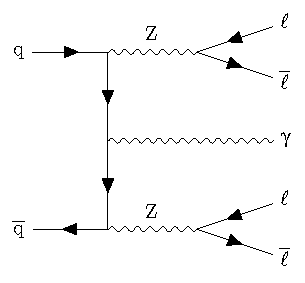
\includegraphics[width=.319\textwidth]{triboson_4LG.pdf} \label{fig:ppTo4LG_hard}}
  \subfigure [From non-abelian coupling]     {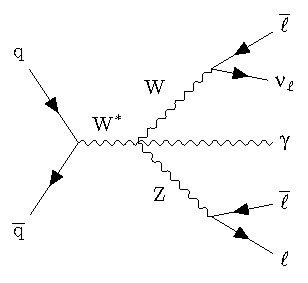
\includegraphics[width=.319\textwidth]{QGC_3LNuG.pdf}    \label{fig:ppTo4LG_GC}  }
  \subfigure [From a final-state fermion]    {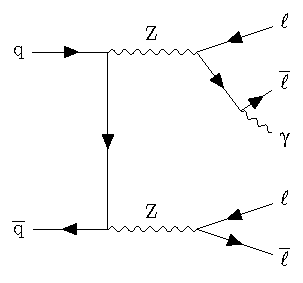
\includegraphics[width=.319\textwidth]{ZZ_4LG.pdf}       \label{fig:ppTo4LG_FSR} }
\caption{Representative Standard Model Feynman diagrams that yield four isolated leptons and a photon in the final state.}
\label{fig:ppTo4LG}
\end{figure}

\paragraph{Signal components\\}
The relative composition of the diagrams shown in Figure~\ref{fig:ppTo4LG} in the signal sample was assessed in a generator level study.
The study is conducted on the four lepton channel, but the results can be generalised to the other two.
Two samples were generated at Leading Order EW ($\alpha_{\rm EW}^5 \, \alpS^0$) using \MADGRAPH.
The first is the inclusive production of four fermions and a photon, while the other constrains the intermediate vector boson state.

More precisely, the first sample simulates the process $\Pp\Pp \to 2\Pe 2\PGm \PGg$,
which in \MADGRAPH syntax corresponds to \verb|generate p p > e+ e- mu+ mu- a|.
The photon may be attached either to an initial- or final-state fermion line,
but not to a triple or quartic vertex since there are no suitable couplings in the SM for this final state.
The choice of a final state where the two lepton pairs have different flavour
excludes the interference from diagrams with the momenta of two leptons swapped.
The computed cross section is $0.075 \fbinv$.

The second sample forces the intermediate Z boson resonances $\Pp\Pp \to \PZ\PZ\PGg \to 2\Pe 2\PGm \PGg$,
using the syntax:
\begin{verbatim}
define ze = z
define zmu = z
generate p p > ze zmu a, ze > e+ e-, zmu > mu+ mu-
\end{verbatim}
In this case the photon is forced to be directly attached to an initial-state fermion line,
making this a sub-sample of the previous one.
The computed cross section is $0.027 \fbinv$.

The distributions of the invariant mass of the same-flavour opposite-sign lepton pairs and the transverse momentum of the photon
for the first and second sample are shown in Figure~\ref{fig:genstudy}.
From these plots it appears that in a sizeable fraction of FSR events the mass of one of the
reconstructed $\Pl\Pl$ pairs is significantly lower than the \PZ peak.
It is also visible that the transverse momentum of FSR photons tends to be lower,
since the momentum of the lepton may change significantly,
and it becomes almost zero above $80\GeVc$.
However only a fraction of the events in both samples are in the tail with $\pt^\PGg > 80\GeVc$.

\begin{figure}
  \centering\hfill
  \subfigure [$m_{\Pl\Pl}$] {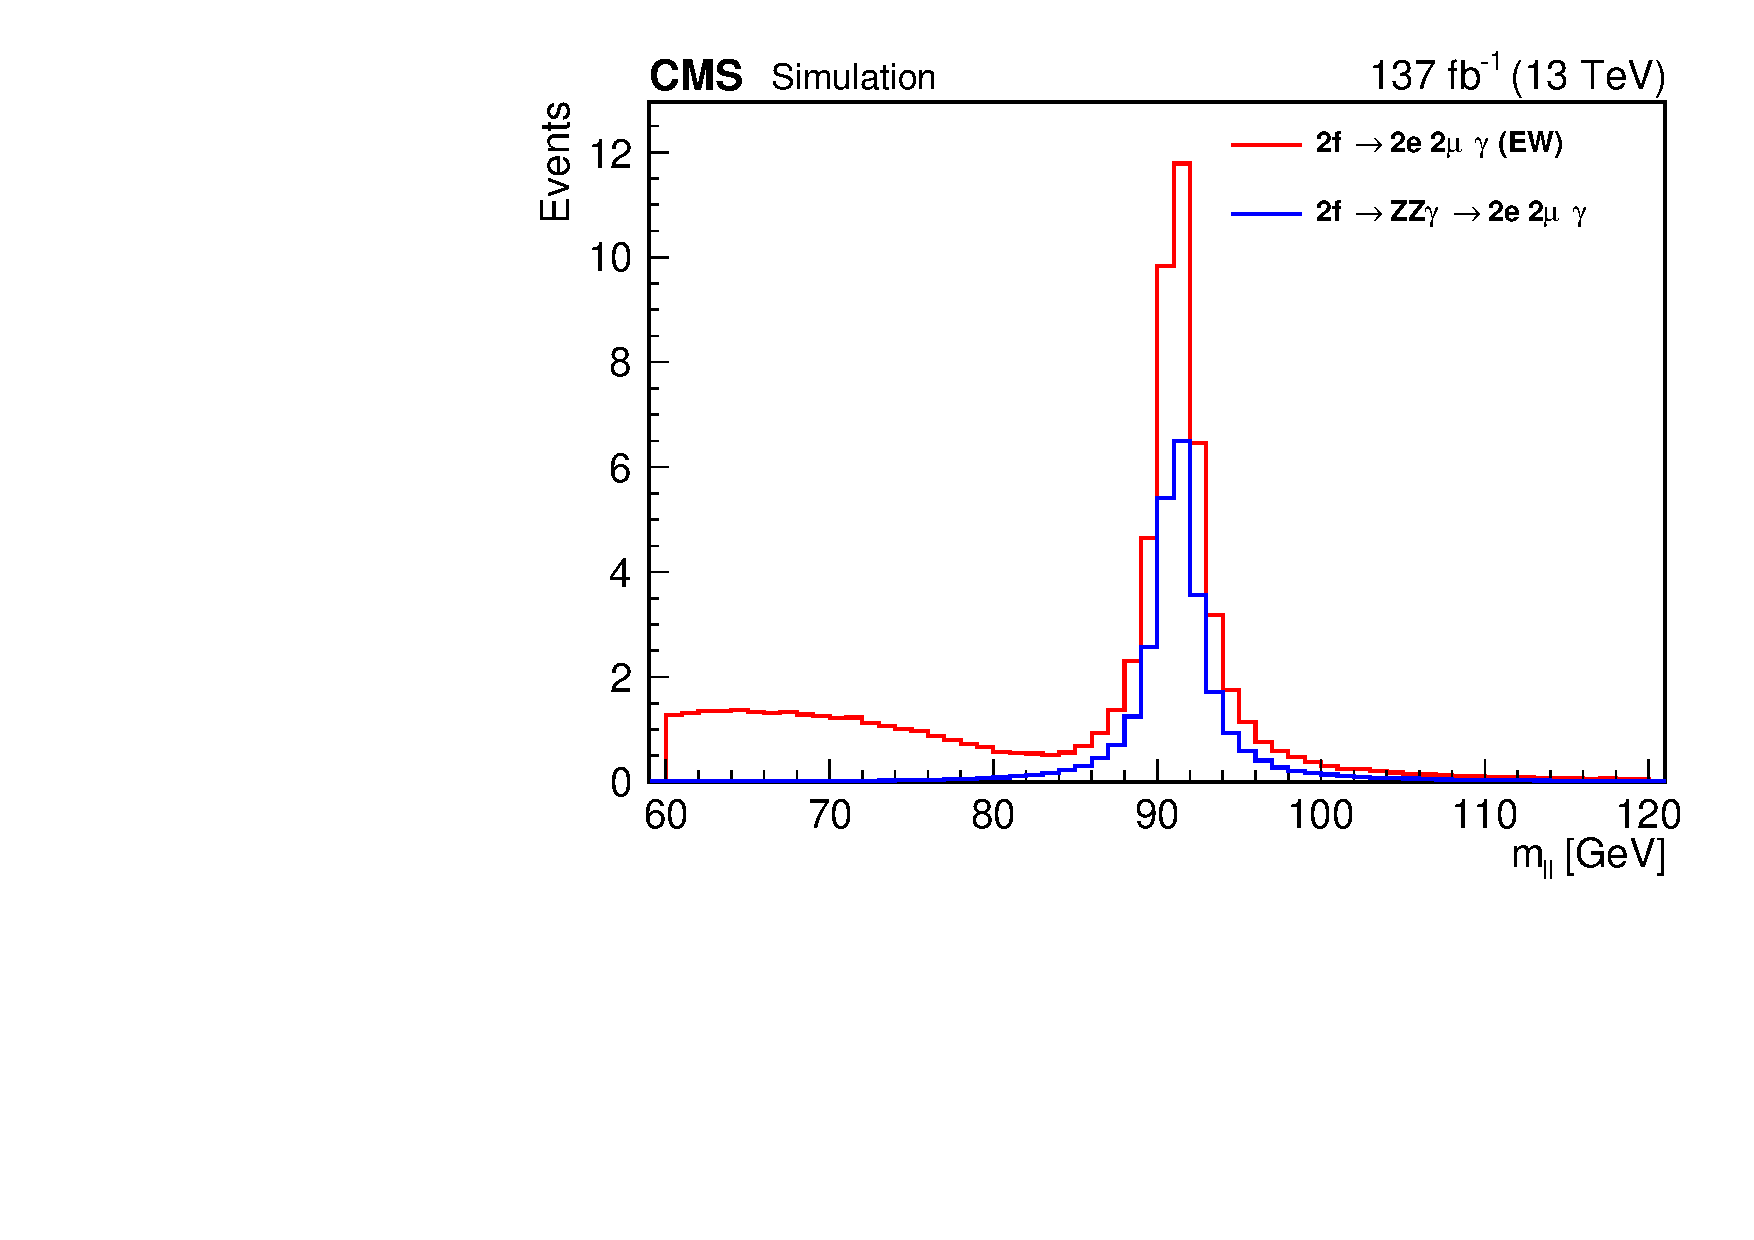
\includegraphics[width=.45\textwidth]{genstudy_mll.pdf}}\hfill
  \subfigure [$\pt^\PGg$]   {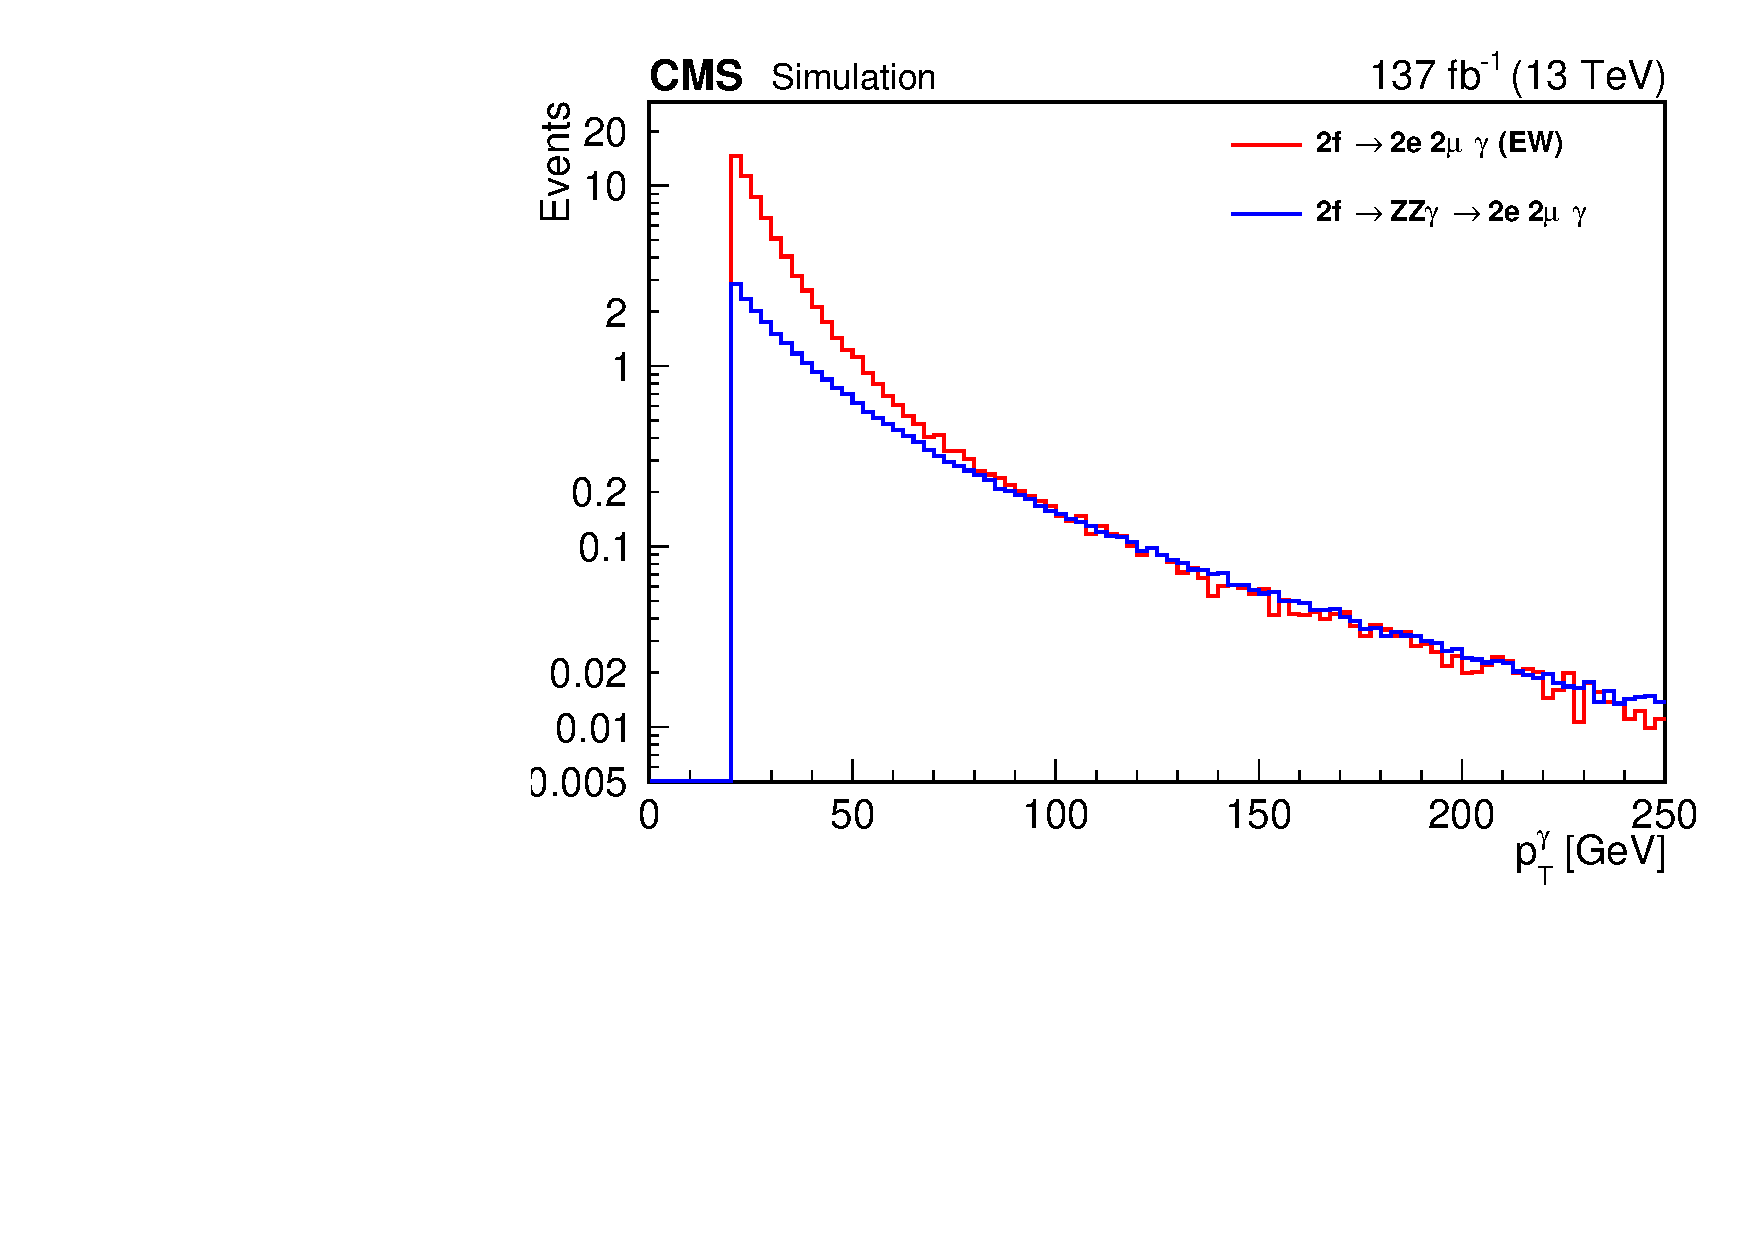
\includegraphics[width=.45\textwidth]{genstudy_ptGamma.pdf}}\hfill\mbox{}
  \caption{Invariant mass of the same-flavour opposite-sign lepton pairs and the transverse momentum of the photon
  in the two MC samples produced for the study of the fraction of FSR events in the $\Pp\Pp \to 4\Pl\PGg$ process.}
  \label{fig:genstudy}
\end{figure}


\subsection{Signal definition}
\label{sec:signal_definition}
% the signal definition at gen level
The fiducial phase space definition mimics the selection applied to reconstructed events, described in Section \ref{sec:event_selection}.

The charged leptons, either electrons or muons are required to have $\pt > 5 \GeV$ and $|\eta| < 2.5$.
Each lepton pair $\Pl_i, \Pl_j$ must be separated $\DR(\Pl_i, \Pl_j) > 0.02$.
\todo{Is this actually done?}
Lepton isolation is ensured by requiring the scalar sum of the \pt of all stable particles, i.e.,
those particles not decaying in the detector volume, within a cone of radius $\DR = 0.3$ to be less than 0.35 times the \pt of the lepton.
\todo{Again, to be checked.}
Neutrinos, FSR photons, and leptons (electrons and muons) are not included in
the computation of the isolation sum to enhance the model independence of the measurements,
following the findings of Reference \cite{HIG-14-028}.
Low mass resonances are excluded by requiring that any opposite-sign lepton pair, regardless of flavour,
satisfies $m_{\Pl^{+} \Pl'^{-}} > 4\GeV$.

The number of charged leptons that pass these requirements is used to categorise the event into one of the three channels: 4\Pl, 3\Pl and 2\Pl.

The photon is required to have $\pt > 20 \GeV$, $|\eta| < 2.4$ and be produced in the hard scattering. % isPrompt
It must be separated from any lepton by $\DR(\PGg, \Pl) > 0.5$.
In all channels it is required the presence of a photon passing these requirements.

Jets are built with the \antikt algorithm with a distance parameter of 0.4,
and are required to have $\pt^{\rm jet} > 30 \GeV$ and $|\eta^{\rm jet}| < 4.7$, as done at the reconstruction level.
The jets are kept if no lepton or photon inside a cone with the size of the jet radius is found.
Large radius jets are built using a distance parameter of 0.8
and are required to have $\pt^{\rm jet} > 150 \GeV$ and $|\eta^{\rm jet}| < 4.7$.

In the 4\Pl channel the leading (sub-leading) lepton must have $\pt > 20\ (10) \GeV$.
There must be two pairs of same-flavour and opposite-sign (SFOS) leptons, which are labelled $\PZ_1$ and $\PZ_2$,
the former being the one with the mass closest the the Z peak, which must have $60 \GeV < m_{\PZ_{1,2}} < 120 \GeV$.

In the 3\Pl channel, the SFOS pair with the mass closest to the \PZ peak is selected first, and the remaining lepton is assigned to the \PW.
The mass of the \PZ boson must be $60 \GeV < m_\PZ < 120 \GeV$. %within 15 \GeV from the \PZ peak.
The leading (sub-leading) lepton from the \PZ boson must have \pt > 20 (10) \GeV,
while the lepton from the \PW must have \pt > 20 \GeV.
The transverse momentum of the neutrino is required to be larger than 30\GeV.

In the 2\Pl channel the two leptons must have same flavour and opposite sign
and the leading (subleading) lepton must have $\pt > 20\ (10) \GeV$.
There must be two jets with a mass such that $50\GeV < m_{jj} < 120\GeV$
or a single large radius jet with a mass in the the same range.

%% NOTE: The following paragraph is wrong
%% In the 2 \Pl channel, the two quarks from the decay of the VB must have $\pt > 30 \GeV$ and $|\eta| < 4.7$.
%% Their flavour must be compatible with a \PZ decay (e.g. \PQu\PAQu, \PQd\PAQd, \PQs\PAQs, \PQc\PAQc or \PQb\PAQb),
%% or a \PW decay (e.g. \PQu\PAQd, \PQu\PAQb, \PQd\PAQu, \PQd\PAQc, \PQs\PAQd or \PQs\PAQc).
%% The separation between the quarks and the photon must be $\DR(\PGg, \PQq) > 0.4$.



\section{Background}
\label{sec:backgrounds}
%% An accurate description of the background process is an essential aspect of any analysis since it affects the extraction of signal yields.
The main background sources differ between the three channels, but can be divided into two categories.

In the first one there are processes which have the same final state as the signal and survive all signal region cuts (\textit{irreducible background}).
These are processes that generate the same stable particles as the signal,
although the kinematic distributions may be different.
Usually processes in this class are estimated with simulation,
but in some cases it is possible to constrain their normalization in a control region.

In the second one fall processes that have a different final state than the signal, but enter in the signal region nonetheless (\textit{reducible background}).
Although the final states are different,
either due to additional particles produced in the same hard scattering
or coming from other collisions in the same bunch crossing (\pileup),
that are reconstructed in the detector and not rejected by the identification algorithms,
they generate events which pass the selection.
This particles can either be \nonprompt leptons or photons, or misidentified light-flavour jets.

\Nonprompt leptons come mainly from decays of heavy flavour mesons and electrons from asymmetric photons conversions,
while \nonprompt photons originate primarily from decays of light neutral mesons like \PGpz or \PGh.
Both leptons and photons in this category tend to be non-isolated from the nearby jet activity.

The other class is comprised of misidentified jets, mostly from light-flavour quarks, which can erroneously be reconstructed as either leptons,
if a track is associated to the main energy deposits, or as photons otherwise.
These misidentified photons tend to have a different energy distribution in the ECAL with respect to real photons,
which makes shower shape variables effective in separating this background from real photons.

In the following the terms \textit{fake leptons} and \textit{fake photons} are used to refer to both \nonprompt and misidentified objects.
These processes have cross sections orders of magnitude larger than the signal.
Often these backgrounds prove difficult to model in simulation,
and it becomes advisable to use a data-driven method for their estimation.

\subsection{Four lepton channel}
For the 4\Pl channel the predominant background component is the production of two on-shell \PZ bosons
which decay to either electrons or muons.
It is possible that and a photon that is either radiated as FSR from one of the leptons
is also present in the event, thus producing the same signature as the signal.
Alternatively the photon may be \nonprompt or a misreconstructed jet.

Two \PZ bosons can be produced through quark-antiquark annihilation, as shown in Figure~\ref{fig:qqtoZZto4L}
or from gluon fusion with a quark loop, illustrated in Figure~\ref{fig:ggtoZZto4L}.
The latter is a Next-to-Leading Order (NLO) process, and its contribution is around 10\usep\% of the former in terms of event yield.

Additional backgrounds such as $\PQt\PAQt\PZ$ and VVV (V = \PZ, \PW) result in very small contributions.

\begin{figure}
\hfill
\subfigure [$\PQq\PAQq \to \PZ\PZ \to 4\Pl$]     {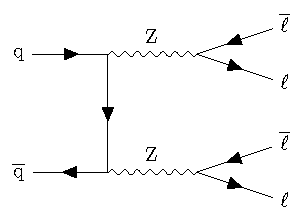
\includegraphics[width=.4\textwidth]{Figures/Feynman/qq_ZZ_4L.pdf} \label{fig:qqtoZZto4L}} \hfill
\subfigure [$\Pg\Pg \to \PZ\PZ \to 4\Pl$ (loop)] {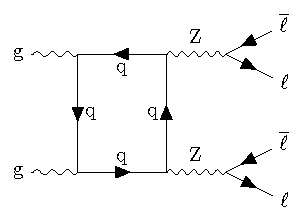
\includegraphics[width=.4\textwidth]{Figures/Feynman/gg_ZZ_4L.pdf} \label{fig:ggtoZZto4L}} \hfill\mbox{}
\caption{Feynman diagrams for the production of two Z bosons
with subsequent decay to four charged leptons
either from quark-antiquark annihilation
or from a gluon-initiated loop.}
\end{figure}

\subsection{Three lepton channel}
In the three lepton channel the main background contributions are $\PW\PZ$, Drell-Yan + jets and $\PZ\PGg$ + jets.
As for the $\PZ\PZ$ in the four lepton channel, in $\PW\PZ$ events an additional photon may be emitted as FSR from one of the leptons
or be a misidentified or \nonprompt particle.
The cross sections of Drell-Yan processes and $\PZ\PGg$ production are much larger than that of the signal and,
although the probabilities of particle misreconstruction or misidentification are comparatively small,
they result in a significant yield in the signal region.

Another not negligible contribution is the $\PZ\PZ \to 4\Pl$ where one of the leptons is lost or misreconstructed as a photon.
There is also a small fraction of events from $\PZ\PZ\PGg$ in which one of the leptons is outside the detector acceptance.
Additional backgrounds from rare processes such as $\PQt\PAQt\PZ$ and VVV (V = \PZ, \PW) result in very small contributions and are estimated with simulation.

\subsection{Two lepton channel}
In the two lepton channel the major background are Drell-Yan processes and $\PZ\PGg$ production.
Unlike the three lepton channel, the absence of the requirements on the presence of the third lepton and of the missing energy
enhances the contributions from these sources.
The main distinguishing feature is the kinematics and characteristics of the hadronic part of the events,
which plays a major role in this channel.


\section{Event selection}
\label{sec:event_selection}

\textbf{Z candidates} are defined as pairs of selected leptons (electrons or muons) with same flavour and opposite sign (SFOS).
They must satisfy $60 < m_{\Pl\Pl} < 120 \GeV$, where the Z candidate mass includes any selected FSR photons associated with its leptons.

\subsection{Four lepton channel}
In the 4\Pl channel, \textbf{ZZ candidates} are built from pairs of Z candidates with no lepton in common.
The first Z candidate $\PZ_1$ is chosen as the one with the reconstructed mass $m_{\Pl\Pl}$ closest to the nominal Z mass.
The second candidate is called $\PZ_2$.
The ZZ candidates are required to satisfy the following:
\begin{itemize}
\item Ghost removal: each of the four leptons must have $\DR > 0.02$ with any of the others.
  This requirement excludes ``ghost tracks'' made with a fraction of the hits of another lepton that produce an additional spurious lepton candidate.
\item Lepton \pt: the most energetic lepton must have $\pt^1 > 20 \GeV$ and the second most energetic $\pt^2 > 10 \GeV$,
  in order to ensure a high and constant trigger efficiency for all the selected events.
\item Low mass resonance suppression: all four opposite sign pairs, regardless of flavour, that can be built must satisfy $m_{\Pl\Pl} > 12 \GeV$.
  This cut suppresses pairs of leptons from cascade decays, which may have different flavour and are found to broadly peak at very low invariant masses.
  In this case, selected FSR photons are not used in computing $m_{\Pl\Pl}$, since a QCD-induced low mass di-lepton (\eg\ \JPsi) may have photons nearby (\eg from a \Pgpz).
\item Wrong pairing suppression: in the 4\Pe and 4\PGm channels,
  it is required that the alternative pairing of the four leptons does not result in
  an on-shell Z and a low mass $\Plp\Plm$ resonance with $m_{\Pl\Pl} < 12 \GeV$.
\item Four-lepton invariant mass: $m_{4\Pl} > 100 \GeV$.
\end{itemize}

\subsection{Three lepton channel}
In the 3\Pl channel the \PZ candidate is built first, using the pair of leptons with same flavour and opposite sign with the mass closest to the Z peak.
If no SFOS pair is found, the event is discarded.
The \PW is built with the third lepton and the MET. %% , which must be higher than 30 \GeV
The {\bf $\PW\PZ$ candidate} must then satisfy the same requirements of ghost removal and low mass resonance suppression imposed to the ZZ candidate in the 4\Pl channel.
Additionally:
\begin{itemize}
\item lepton \pt: the two leptons from the \PZ boson must have $\pt^{\Pl_{Z,1}} > 25 \GeV$ and $\pt^{\Pl_{Z,2}} > 10 \GeV$,
  while the lepton in the \PW must have $\pt^{\Pl_{\PW}} > 25 \GeV$.
  As for the four lepton channel, this is to ensure high and constant trigger efficiency, by having at least two leptons ($\Pl_{Z,1}$ and $\Pl_\PW$)
  be above the threshold for the most energetic lepton of all the dilepton triggers,
  and that the third is above the less stringent threshold for the second lepton of such trigger paths.
\item \PZ mass: the \PZ boson mass must be within $15 \GeV$ from the \PZ mass peak.
\item Minimum MET: the missing energy must be $\ptmiss > 30 \GeV$.
\item Three-lepton invariant mass: the invariant mass of the system of the three charged leptons is required to be $m_{3\Pl} > 100 \GeV$.
  This effectively suppresses contributions from $\PZ\PGg$ production where there is an asymmetric conversion of the photon that produces an electron.
\item b-veto: Events are rejected if there is at least one jet passing the medium b-tag threshold (see Section~\ref{sec:jet_ID}).
  This is meant to suppress top quark backgrounds, like $\PQt\PAQt\PZ$ or $\PQt\PZ\PQq$ with a jet misidentified as photon.
\end{itemize}

\subsection{Two lepton channel}
The \PZ boson is build with the two leptons, which must be a SFOS pair.

The reconstruction of the hadronically decaying vector boson is intrinsically challenging,
since the large number of particles inside the jets degrades the resolution as compared to energetic and isolated leptons.
Furthermore, jet energy is sensitive to \pileup, both from charged and neutral particles, which must be accounted for.

When the vector boson is significantly boosted, the two quarks tend to be emitted with a small angle between them,
and thus the two jets have a small separation in \DR, causing them to overlap.
In this case, sometimes the clustering algorithm is not able to distinguish the two jets or cannot reconstruct them correctly.
Instead, it creates a single cluster, which often does not contain all the particles, and underestimates the energy of the jet.

For this kind of topology, one possible approach consists of running again the clustering algorithm with a larger value of the distance parameter D,
which is more likely to be able to include in an unique larger jet the particles coming from the quarks hadronization.
This creates a new set of jets which constitutes an alternative vision of the hadronic part of the event.

\begin{figure}
\centering
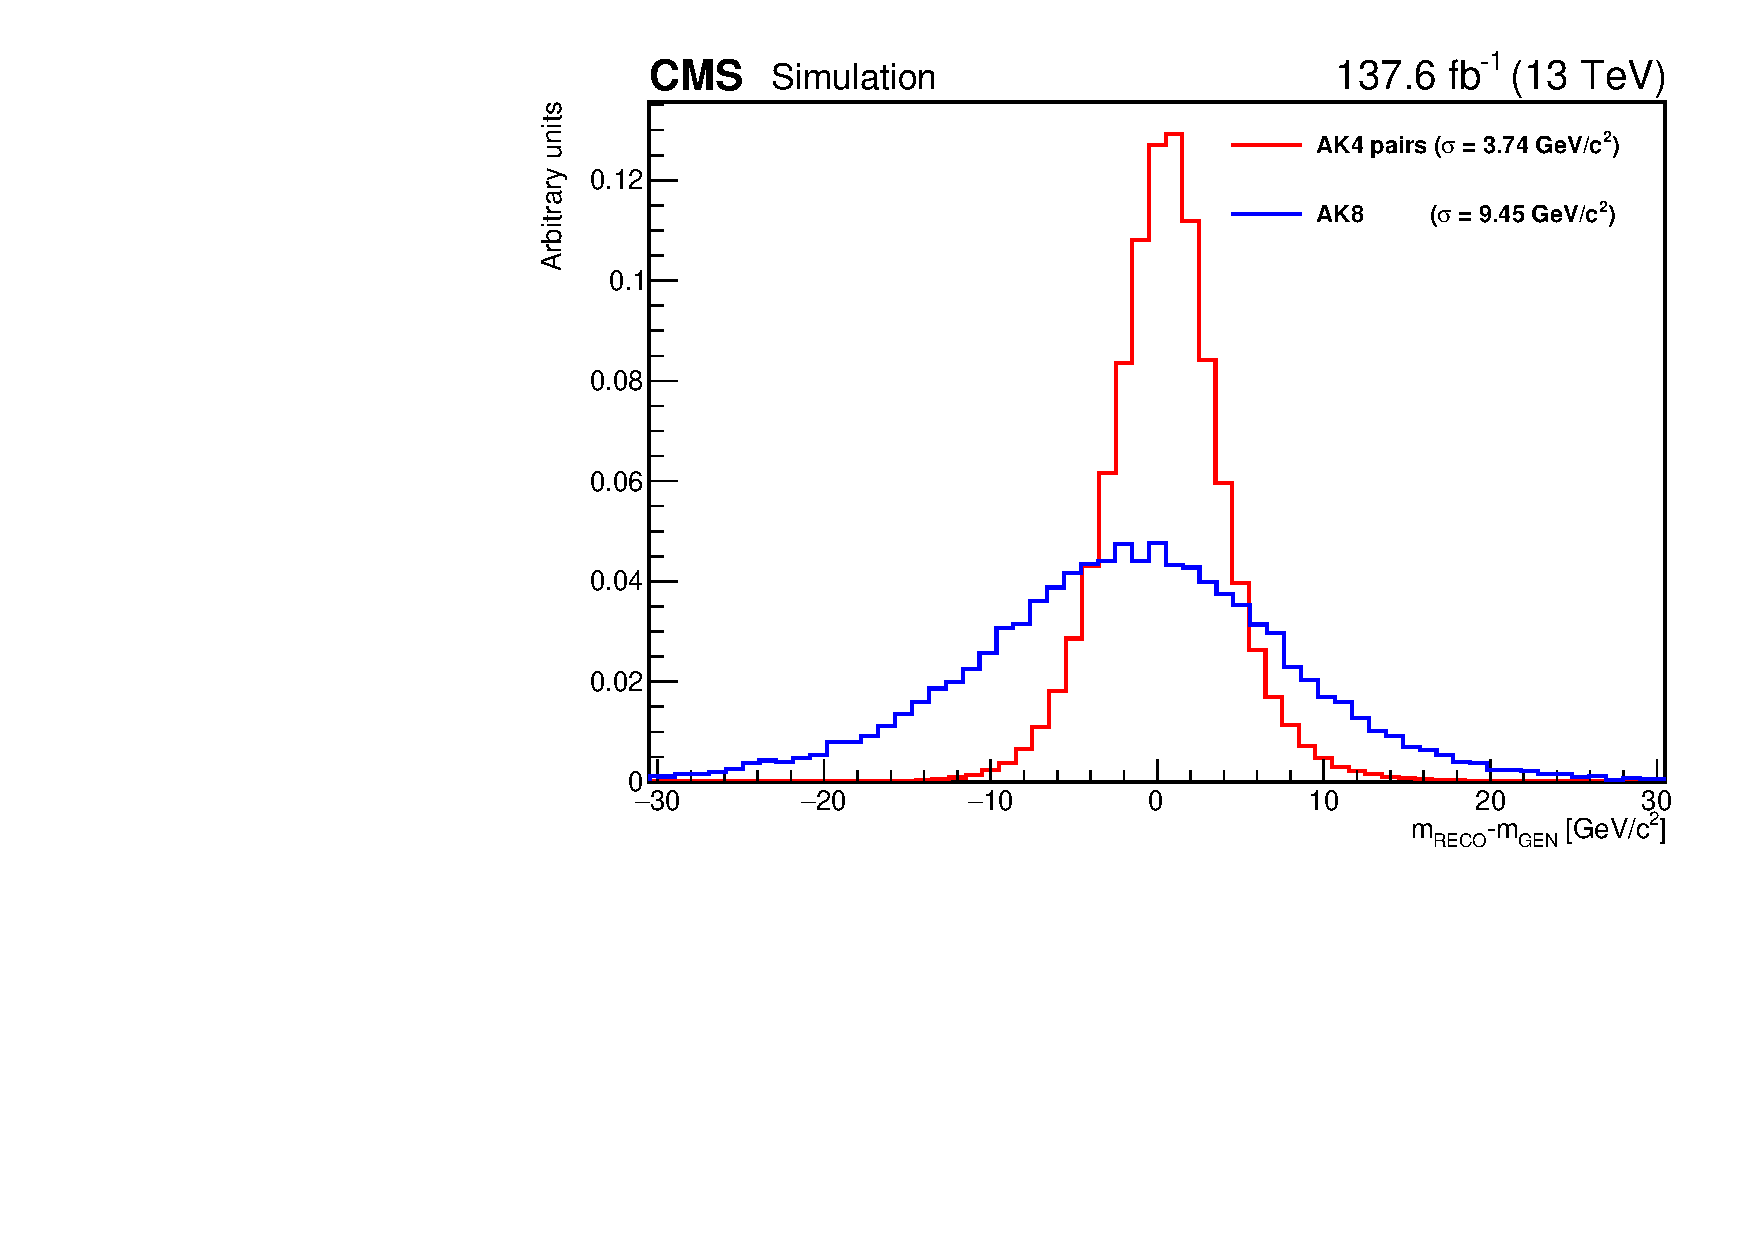
\includegraphics[width=0.5\textwidth]{AK_resolution_mass.pdf}
\caption{Resolution of the mass of reconstructed AK8 jets and pairs of AK4 jets, with respect to the generated objects.
The events correspond to the simulation of $\PZ\PZ\PGg \to 2\Pl\, 2j\, \PGg$ for the \RunII{} data taking period.
The two histograms are normalized to have unit area.}
\label{fig:AK_resolution_mass}
\end{figure}

From Figure~\ref{fig:AK_resolution_mass}, it is clear that pairs of AK4 jets are more precise in the reconstruction of the mass of the bosons.
This is caused by the larger number of \pileup{} particles included in a AK8 jet, which in turn require larger energy corrections or pruning, thus increasing the uncertainty.
Additionally the vector boson often does not have a very high transverse momentum,
so the resolved topology is more probable than the merged one.

\subsection{Photon selection}
\label{sec:evt_photon_selection}
The photon selection is common to the three channels.
Photons are required to have a transverse momentum $\pt^\PGg > 20 \GeV$
and be in the acceptance region of the ECAL, excluding the overlap region, $|\eta^\PGg| < 1.442$ or $1.566 < |\eta^\PGg| < 2.4$.
The minimum separation between a photon and any of the leptons must be $\DR(\PGg, \Pl) > 0.5$.
Photons are required to pass the Conversion Safe Electron Veto,
which prohibits tracks pointing to the photon ECAL cluster,
unless matched to a photon conversion vertex~\cite{CMS-EGM-17-001}.
%% and the Pixel Seed veto

Several photon identification algorithms are compared in this analysis (see Section~\ref{sec:photon_selection}):
the Loose working point of the cut-based ID
and the two working points \texttt{wp90} and \texttt{wp80} of the MVA-based ID.
In case there is more than one photon passing the requirements, the one with the highest \pt is selected.

For the results on the significance of triboson production, the cut designed to suppress FSR contributions
described in Section~\ref{sec:FSR_cut} is also applied.


\section{Background estimation strategy}
I devised a set of background estimation strategies mainly for misidentified and \nonprompt particles that are common to the three channels.
The consequent division into Signal Regions (SR), Control/application Regions (CR) and measurement region is illustrated in Table~\ref{tab:region_definition}.
\begin{table}
  \caption{
    Definition of the division into channels and regions adopted in the analysis.
    The rows ``PASS'' and ``FAIL'' refer to whether the photon passes or fails the tight analysis selection.
    The lepton status follows the same principle, with separate columns signifying a different combination of leptons that pass or fail the tight selection.
    Each group of columns, characterised by a different number of leptons passing at least the loose selection, is a channel.
    The three lepton channel is further divided depending on whether the $\ptmiss$ is larger or smaller than 30\GeV.
    The latter contains the $3\Pl$ signal region,
    while the latter encompasses the lepton and photon fake rate measurement region.
  }
  \label{tab:region_definition}
  \resizebox{\textwidth}{!}{%
    \begin{tabular}{|c | c|c|c | c|c|c|c | c|}
      \hline
      channel $\rightarrow$    & \multicolumn{3}{c|}{4 \Pl} & \multicolumn{4}{c|}{3 \Pl $\ (\ptmiss > 30 \GeV)$} & 2 \Pl   \\
      \hline
      \Pl status $\rightarrow$ & 4P      & 3P1F & 2P2F      & 3P      & 2P1F & 2P2F & 3F                        & 2P      \\
      \hline
      \PGg PASS                & \cellcolor[HTML]{cc7fff}SR & \multirow{2}*{CR \Pl} & \multirow{2}*{CR \Pl} &
                                 \cellcolor[HTML]{a4c2f3}SR & \multirow{2}*{CR \Pl} & \multirow{2}*{CR \Pl} & \multirow{2}*{CR \Pl}  &
                                 \cellcolor[HTML]{ffcb7f}SR \\
      \cline{1-2} \cline{5-5} \cline{9-9}
      \PGg FAIL                & CR \PGg &      &           & CR \PGg &      &      &                           & CR \PGg \\
      \hline %% \midrule
      \multicolumn{3}{c}{}                                & & \multicolumn{4}{c|}{3 \Pl $\ (\ptmiss < 30 \GeV)$} & \multicolumn{1}{c}{} \\
      \cline{5-8}
      \multicolumn{3}{c}{}                                & & 3P & 2P1F & 1P2F & 3F                             & \multicolumn{1}{c}{} \\
      \cline{5-8}
      \multicolumn{3}{c}{}                                & & \multicolumn{2}{c|}{\shortstack[c]{\vspace{.5ex} \\ \Pl-FR and \PGg-FR \\ measurement}} & & & \multicolumn{1}{c}{} \\
      \cline{5-8}
    \end{tabular}
  }
\end{table}


\subsection{Fake leptons}
\label{sec:fake_leptons}
To estimate the expected fake lepton background yield in the signal region,
dedicated control regions are defined with requirements similar to the signal region but in such a way not to contain signal events.
To enhance the \nonprompt lepton component, events in these regions are required to
have a number of leptons that fail the tight selection, while passing the loose criteria.
The other selections are identical to maintain similarity with the signal region.

The fake lepton background yield in the signal region is extrapolated from these regions
according to the probability for loose lepton candidates to pass also the final selection criteria,
defined in Sections~\ref{sec:ele_selection} and \ref{sec:muo_selection} for electrons and muons respectively.
These probabilities, referred to as fake rates, are estimated independently as illustrated in the following section.

\subsubsection{Lepton fake rate measurement}
\label{sec:CRLFR}
The measurement of the lepton fake rate, which is the probability that a fake lepton that passes the loose selection also passes the tight criteria,
is carried out in a separate control region which is enriched in contempt leptons.

This region, denoted as $\PZ+L$, is defined as containing a valid \PZ candidate whose leptons must have $\pt^{\Pl_{Z,1}} > 20 \GeV$ and $\pt^{\Pl_{Z,2}} > 10 \GeV$
and an additional lepton which passes the loose selection.
Additionally, the \PZ candidate must have a mass within 10\GeV from the nominal peak,
and the missing energy must be $\MET < 20 \GeV$ to reduce the contribution from real leptons from $\PW\PZ$.
The last requirement means that this region is orthogonal to all of the regions in the 3\Pl channel, in which the MET is required to be greater than 30\GeV.

The fake rate is measured on the third lepton in several bins of transverse momentum, separately for the barrel and endcap and flavour.
The measurement is done for each year of data taking, and the resulting rates can be seen in Figure \ref{fig:leptonFR}.

\begin{figure}
  \centering
  \subfigure [2016] {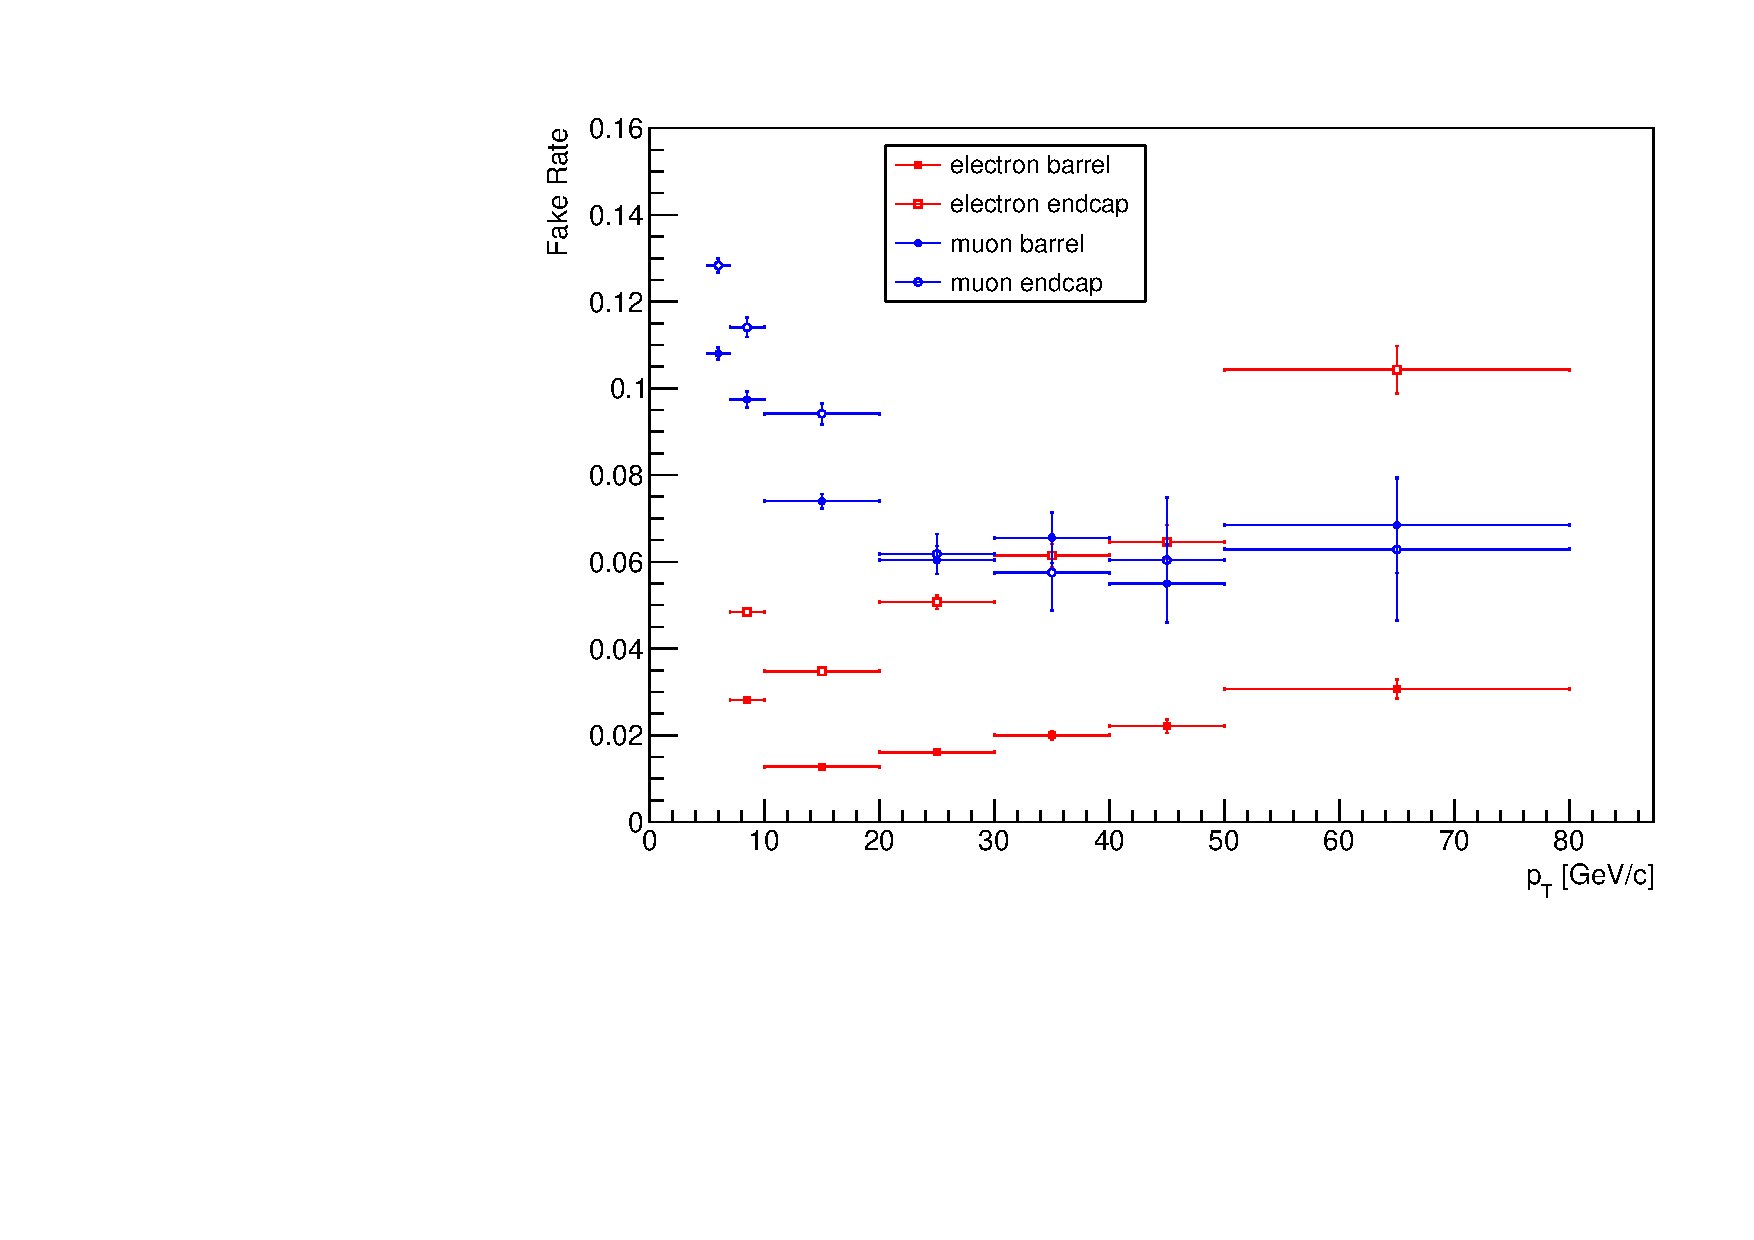
\includegraphics[width=.5\textwidth]{leptonFakeRate_2016.pdf}}%
  \subfigure [2017] {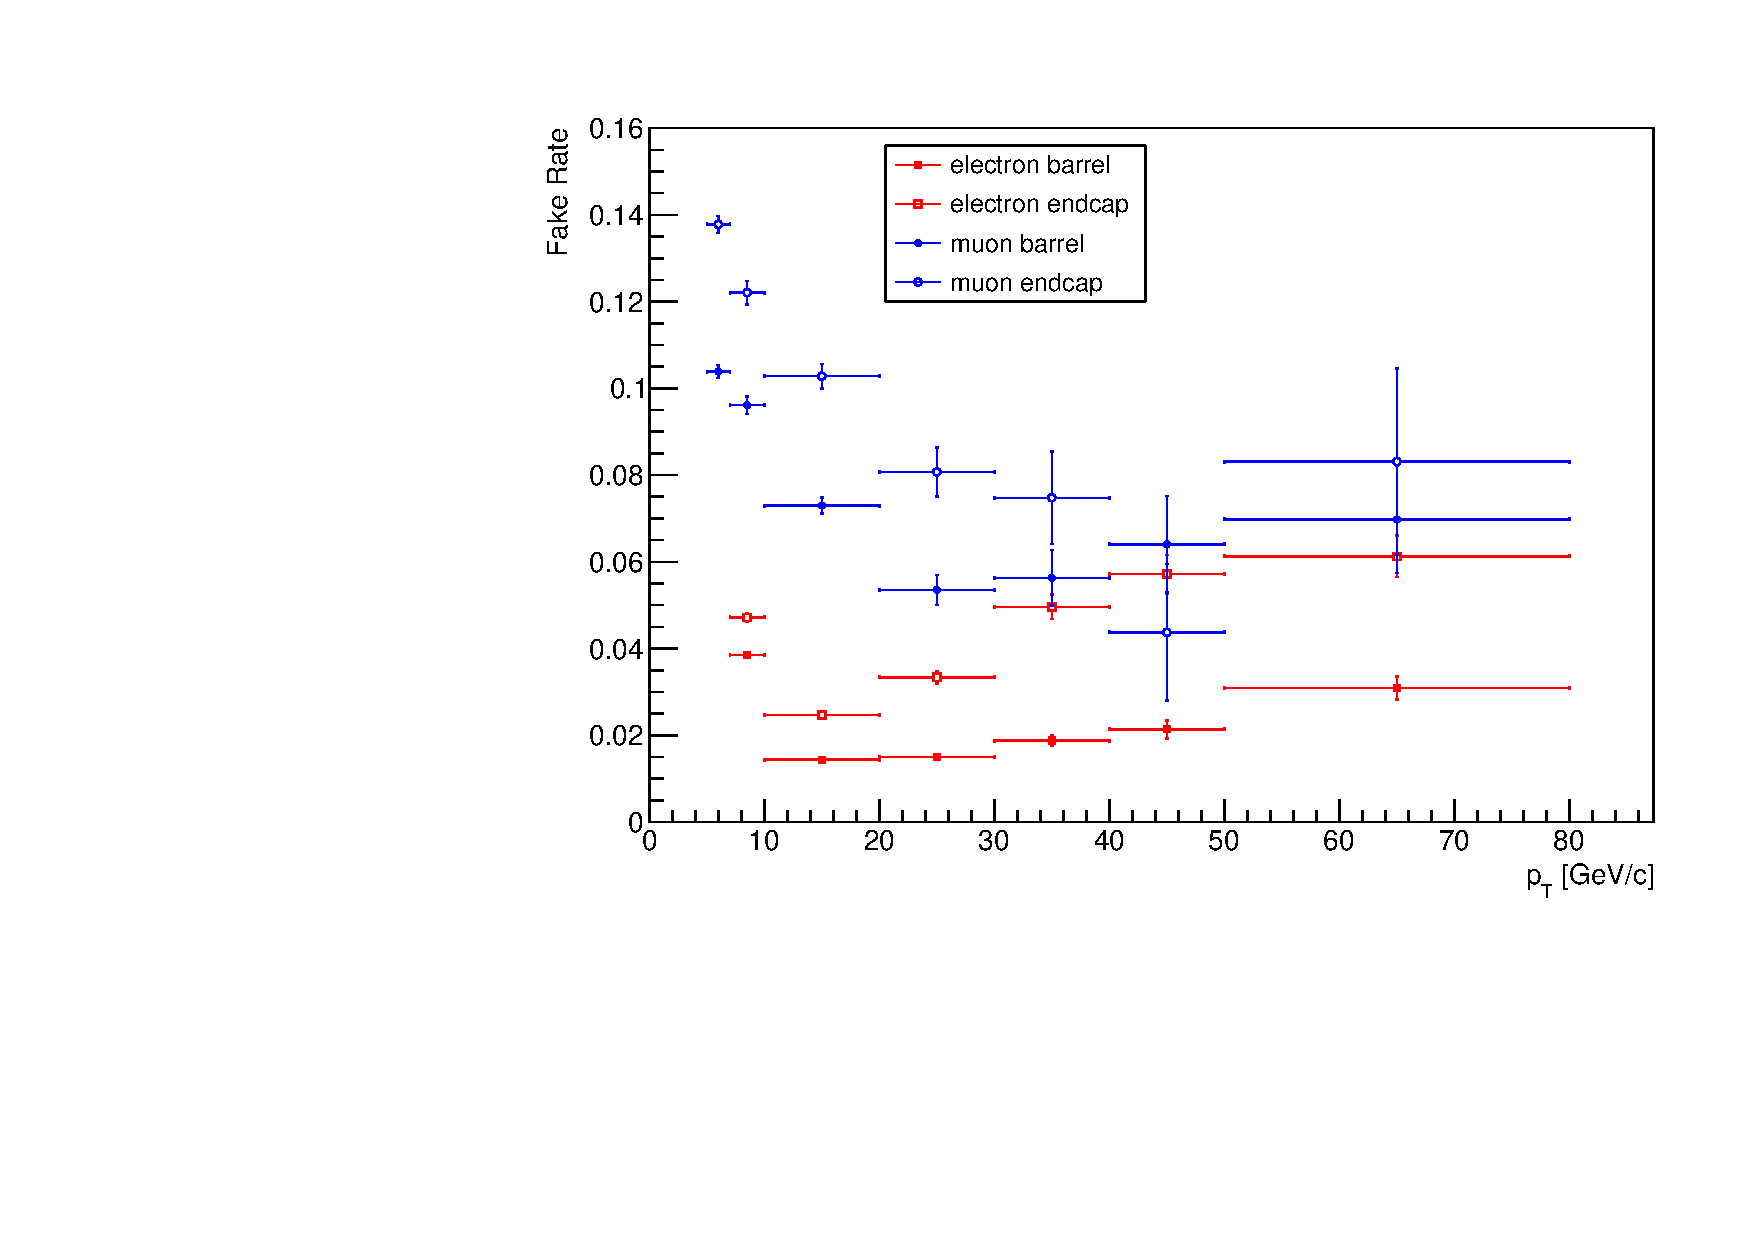
\includegraphics[width=.5\textwidth]{leptonFakeRate_2017.pdf}}\\
  \subfigure [2018] {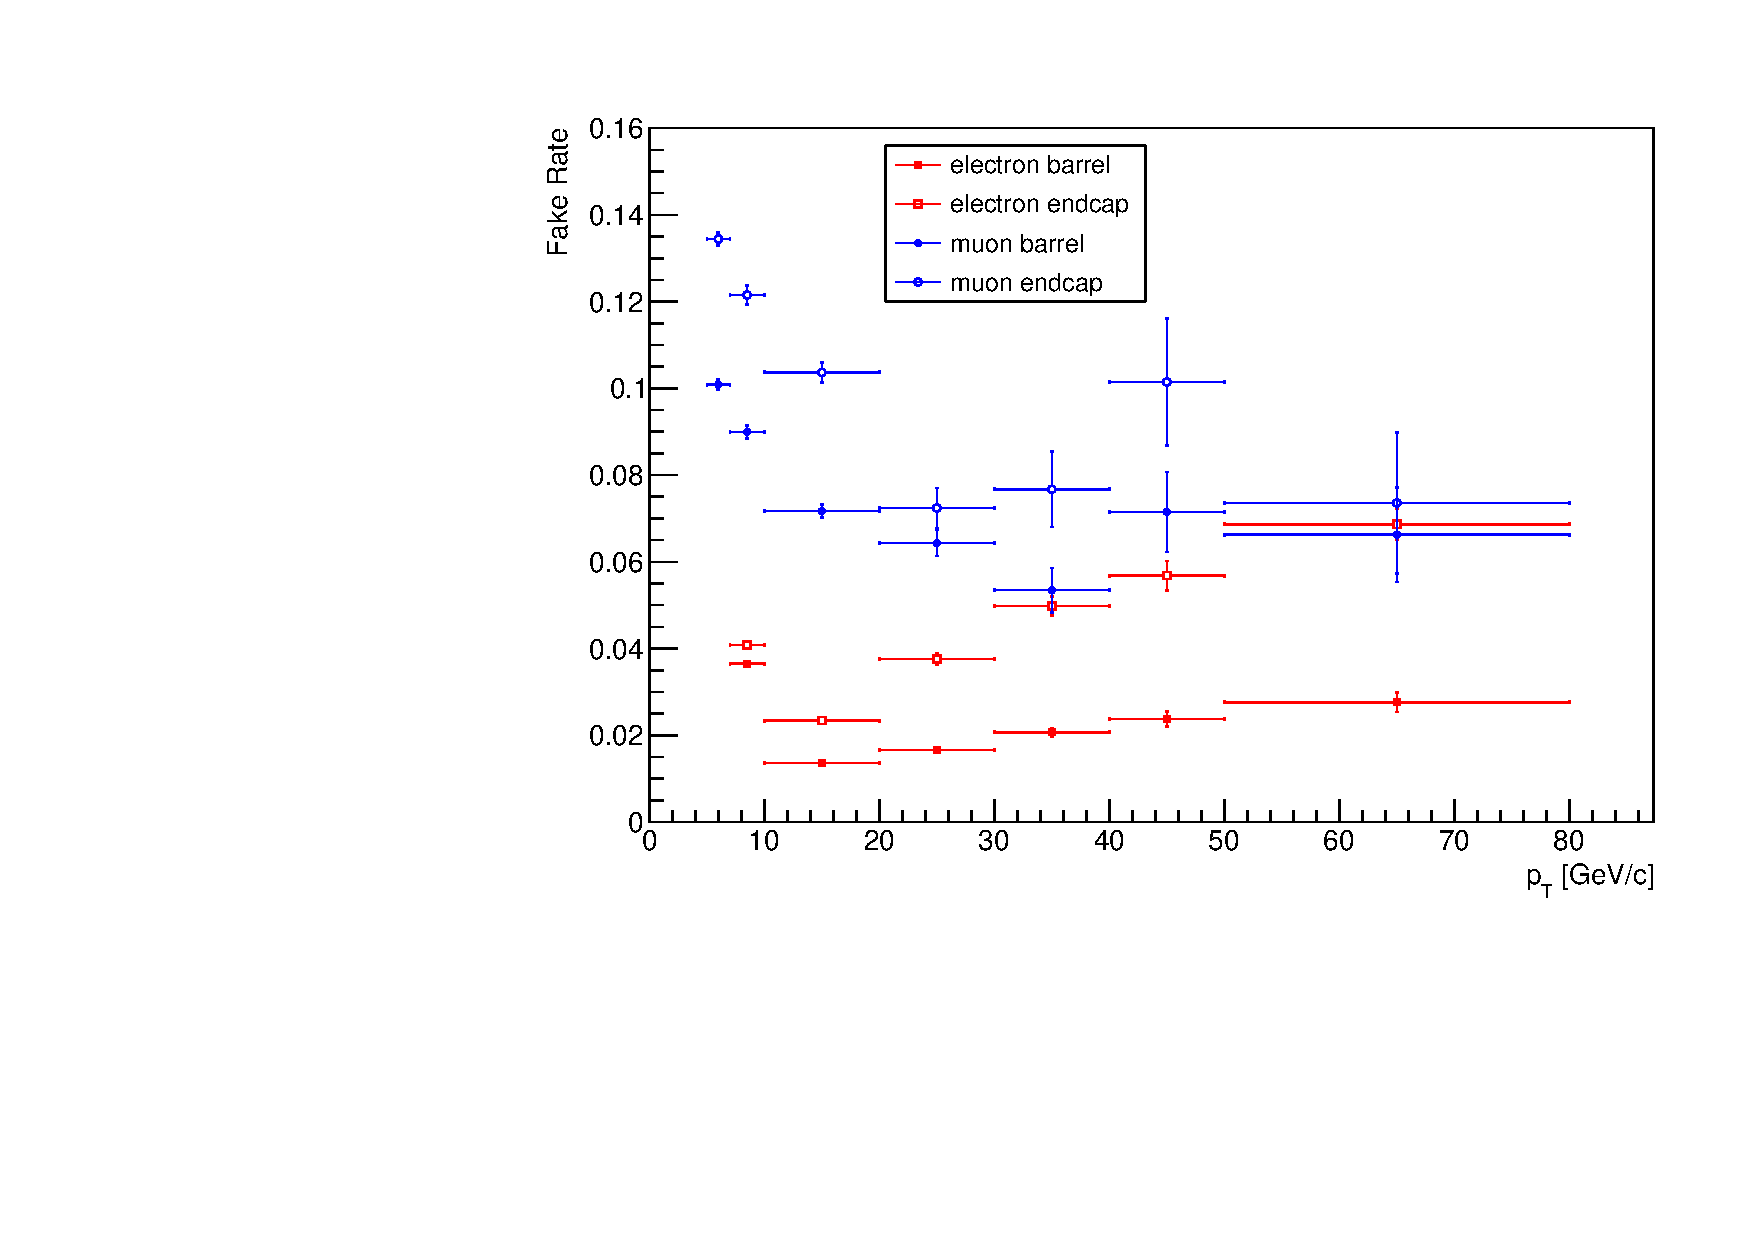
\includegraphics[width=.5\textwidth]{leptonFakeRate_2018.pdf}}
  \caption{Lepton fake rates measured in the $\PZ+L$ control region, for each year of data-taking.}
  \label{fig:leptonFR}
\end{figure}

The uncertainty on the fake lepton background estimation arises from the difference in composition of the
background processes in the region where the fake rate is measured and where it is applied.
This uncertainty was measured by several analyses \todo{cite} and found to be \todo{how much?}.


\paragraph{Lepton fake rate application\\}
Once the fake rates are estimated they are used to reweight the events
in dedicated control regions (alternatively called application regions).

\subsubsection{Four leptons channel}
% Description of the leptonic control regions with 4 leptons:
%  - the backgrounds
%  - data/MC plots
%  - table with fake_lepton background yield foreach year

\label{sec:lepCR4l}
Two control regions are defined for the 4\Pl channel with the same requirements as the signal region
except for the selection of one or more leptons, so as to be enriched in \nonprompt and misidentified leptons.
This method was used by several analyses targeting a final state with four leptons from $\PZ\PZ$ decay~\cite{CMS-SMP-16-001, CMS-SMP-17-006, CMS-SMP-20-001, CMS-PAS-SMP-22-001},
and is described in detail in Reference~\cite{CMS-HIG-13-002} as the ``Method using opposite-sign (OS) leptons''.

\paragraph{CR3P1F\\}
In the first region, named CR3P1F, one of the leptons of the $\PZ_2$ must fail (1F) the tight selection,
while the other three (both leptons from $\PZ_1$ and the other lepton from $\PZ_2$) must pass the tight identification and isolation criteria (3P).
It is expected to be populated by $\PW\PZ$, with contributions from Drell-Yan and $\PZ\PGg$,
along with a fraction of events from $(\PQq\PAQq/\Pg\Pg) \to \PZ\PZ$ where one of the prompt leptons fails the selection
or falls outside the acceptance and a misidentified jet is reconstructed instead.
Distributions of a few interesting kinematic observables are shown in Figure~\ref{fig:CR3P1F_Run2}.

\begin{figure}
\subfigure [$m_{\PZ_1}$     ] {\includegraphics[width=.333333333\textwidth]{Figures/dataMC_noLFR/Run2/fullMC/CR3P1F/Z0_mass_pow.pdf}}%
\subfigure [$m_{\PZ_2}$     ] {\includegraphics[width=.333333333\textwidth]{Figures/dataMC_noLFR/Run2/fullMC/CR3P1F/Z1_mass_pow.pdf}}%
\subfigure [$m_{\PZ\PZ\PGg}$] {\includegraphics[width=.333333333\textwidth]{Figures/dataMC_noLFR/Run2/fullMC/CR3P1F/ZZG_mass_loosePh_pow.pdf}}
\caption{Invariant mass of the $\PZ_1$, $\PZ_2$ (left and centre) without any request on the presence of a photon
  and mass of the $\PZ\PZ\PGg$ system (right) when there is a photon passing the cut-based ID selection,
  in the leptonic control region CR3P1F where one of the leptons from $\PZ_2$ fails the tight selection.}
\label{fig:CR3P1F_Run2}
\end{figure}

\paragraph{CR2P2F\\}
In the second region, named CR2P2F, both leptons from the $\PZ_2$ fail the tight selection (2F), while the leptons of the $\PZ_1$ pass the tight criteria (2P).
This region is populated primarily by Drell-Yan events, with contributions from $\PZ\PGg$ and $\PQt\PAQt+X$.
Some representative distributions for this region are shown in Figure~\ref{fig:CR2P2F_Run2}

\begin{figure}
\subfigure [$m_{\PZ_1}$     ] {\includegraphics[width=.333333333\textwidth]{Figures/dataMC_noLFR/Run2/fullMC/CR2P2F/Z0_mass_pow.pdf}}%
\subfigure [$m_{\PZ_2}$     ] {\includegraphics[width=.333333333\textwidth]{Figures/dataMC_noLFR/Run2/fullMC/CR2P2F/Z1_mass_pow.pdf}}%
\subfigure [$m_{\PZ\PZ\PGg}$] {\includegraphics[width=.333333333\textwidth]{Figures/dataMC_noLFR/Run2/fullMC/CR2P2F/ZZG_mass_loosePh_pow.pdf}}
\caption{Invariant mass of the $\PZ_1$, $\PZ_2$ (left and centre) without any request on the presence of a photon
  and mass of the $\PZ\PZ\PGg$ system when there is a photon passing the cut-based ID selection,
  in the leptonic control region CR2P2F where both leptons from $\PZ_2$ fail the tight selection.}
\label{fig:CR2P2F_Run2}
\end{figure}

\paragraph{Contribution to signal region\\}
The expected reducible background in the signal region is given by the sum of two terms:
\begin{itemize}
  \item A 3P1F component, from events with one fake lepton, estimated from the CR3P1F region.
  \item A 2P2F component, from events with two fake leptons, estimated from the CR2P2F region.
\end{itemize}

The 3P1F and 2P2F components are given by the number of events in the respective regions, weighted by factors dependent on the fake rates:
\begin{subequations}
  \begin{align}
    \label{eq:lepFR_3P1Fto4P}
    N^{\text{from 3P1F}}_{\text{SR}} &= \sum_{i \ins \text{3P1F}} \frac{f_a^i}{1-f_a^i}, \quad \text{where } a = 3 \text{ or } 4
    \\
    \label{eq:lepFR_2P2Fto4P}
    N^{\text{from 2P2F}}_{\text{SR}} &= \sum_{i \ins \text{2P2F}} \frac{f_3^i}{1-f_3^i} \frac{f_4^i}{1-f_4^i}
  \end{align}
\end{subequations}
where $f_3^i$ and $f_4^i$ correspond to the fake rates of the two loose leptons in the $i$-th event.

However, the CR3P1F region itself has a contribution from fake lepton background events from the CR2P2F region.
These are events with two genuine leptons and two fakes, where only one of the fakes passes the tight selection, thus winding up in the CR3P1F region.
The expected number of background events in the CR3P1F region, $N^{\text{from 2P2F}}_{\text{3P1F}}$,
can be computed from the number of events observed in the CR2P2F control region, $N^{\text{bkg}}_{\text{2P2F}}$,
by weighting each event in the region with a factor dependent from the fake rates:
\begin{equation}
  \label{eq:lepFR_N3P1F}
  N^{\text{from 2P2F}}_{\text{3P1F}} = \sum_{i \ins \text{2P2F}} \left( \frac{f_3^i}{1-f_3^i} + \frac{f_4^i}{1-f_4^j} \right)
\end{equation}

Summing all the contributions, one obtains for the signal region:
\begin{equation}
  \begin{split}
    \label{eq:lepFR_4P}
    N^{\text{bkg}}_{\text{SR}} &= \sum_{i \ins \text{3P1F}} \frac{f_a^i}{1-f_a^i} \left( 1 - N^{\text{from 2P2F}}_{\text{3P1F}} \right)
                               + \sum_{i \ins \text{2P2F}} \left( \frac{f_3^i}{1-f_3^i} \frac{f_4^i}{1-f_4^i} \right)
    \\
                 &= \sum_{i \ins \text{3P1F}} \frac{f_a^i}{1-f_a^i} - \sum_{i \ins \text{2P2F}} \left( \frac{f_3^i}{1-f_3^i} \frac{f_4^i}{1-f_4^i} \right)
  \end{split}
\end{equation}

More details on the derivation of Equation~\ref{eq:lepFR_4P} can be found in Appendix~\ref{sec:leptonFR_details}.


\subsubsection{Three leptons channel}
\label{sec:lepCR3l}
\note{At the moment, the data-driven fake estimate does NOT work in SR3P. Maybe we shouldn't discuss it if we don't use it.}

\note{SMP-16-002~\cite{SMP-16-002} (2015 data) uses a dijet region to measure the fake rate:
\textit{``The misidentification probability is measured from a sample of
dijet events enriched in nonprompt leptons. The sample is selected
with one jet passing the relaxed lepton identification requirements
matched to a single lepton trigger, defined as the probe lepton.''}}

\note{SMP-20-014~\cite{SMP-20-014} (full Run2) uses a L+j region:
\textit{``This CR is defined by requiring a single lepton with pT greater than 10 GeV, and at least
a reconstructed jet that is well separated from the lepton at $\DR(\PGg, j) > 0.7$. Contributions from
EWK processes are subtracted to obtain a pure nonprompt measurement region.''}}

Seven leptonic control regions are defined for the three lepton channel, following the strategy used in Reference~\cite{SMP-20-014},
using the same selections as the signal region except for the lepton identification.
The leptons are ordered: $\Pl^\PZ_1$, $\Pl^\PZ_2$ and $\Pl^\PW$
and the regions are defined based on which lepton fails the tight selection.
Unlike the four lepton channel the order is important,
so for example an event where only the leading lepton from the \PZ fails will be in a different control region
from an event where only the subleading lepton does not pass the tight selection.

This classification produces three regions where only one lepton fails the selection, three where two leptons fail and one where all three leptons are \nonprompt.
The agreement between the simulation and the data decreases accordingly, given the instrumental nature of this background, which makes it difficult to model.

\begin{figure}
  \subfigure [$\Pl^\PW$ fails  ] {\includegraphics[width=.333333333\textwidth]{Figures/dataMC_noLFR/Run2/fullMC/CR110/lll_mass_pow.pdf}}%
  \subfigure [$\Pl^\PZ_1$ fails] {\includegraphics[width=.333333333\textwidth]{Figures/dataMC_noLFR/Run2/fullMC/CR011/lll_mass_pow.pdf}}%
  \subfigure [$\Pl^\PZ_2$ fails] {\includegraphics[width=.333333333\textwidth]{Figures/dataMC_noLFR/Run2/fullMC/CR101/lll_mass_pow.pdf}}
  \caption{Invariant mass of the three charged leptons in the three lepton control regions for the 3L channel where only one lepton fails the selection.}
  \label{fig:CR3L_1_Run2}
\end{figure}

\begin{figure}
  \subfigure [$\Pl^\PZ_1$ and $\Pl^\PZ_2$ fail] {\includegraphics[width=.333333333\textwidth]{Figures/dataMC_noLFR/Run2/fullMC/CR001/lll_mass_pow.pdf}}%
  \subfigure [$\Pl^\PZ_1$ and $\Pl^\PW$ fail  ] {\includegraphics[width=.333333333\textwidth]{Figures/dataMC_noLFR/Run2/fullMC/CR010/lll_mass_pow.pdf}}%
  \subfigure [$\Pl^\PZ_2$ and $\Pl^\PW$ fail  ] {\includegraphics[width=.333333333\textwidth]{Figures/dataMC_noLFR/Run2/fullMC/CR100/lll_mass_pow.pdf}}
  \caption{Invariant mass of the three charged leptons in the three lepton control regions for the 3L channel where two leptons fail the selection.}
  \label{fig:CR3L_2_Run2}
\end{figure}


\subsubsection{Two leptons channel}
\label{sec:lepCR2l}
The preliminary strategy for the two lepton channel is to use a data-driven estimate of fake photons
which, as described in Section~\ref{sec:backgrounds_in_SR}, does not need the data-driven estimate of \nonprompt leptons.

A potential strategy for the estimation of the fake lepton contribution in the signal region of this channel was formulated,
emloying employing procedures similar to those applied in the other two.
The fake rate measured in the $\PZ+\rm{L}$ region is applied to reweight events in two control regions: CR1P1F and CR0P2F.
These regions contain a massive amount of events.
The region CR1P1F in particular has a significant contribution from $\PW+\text{jets}$ events,
while the CR0P2F is dominated by QCD-induced jet production.
The event weights applied to derive the contribution to the signal region are the same used in the four lepton channel,
which account for the contamination of the region with one lepton failing the tight selection from events with two fake leptons.



\subsection{Fake photons}
\label{sec:fake_photons_background}
The background from fake photons, either misidentified or \nonprompt, can be estimated using a similar data-driven approach.
It is necessary to define two working points, one being the loose selection and the other the tight analysis selection.
For this analysis, the Loose working point of the cut-based ID is the tight analysis selection,
while the \textit{very loose} selection (see Section \ref{sec:photon_selection}) is used as the loose criterion.
The differences between the two selections are the two cuts on the shower shape variable \sieie
and on the ratio of hadronic to electromagnetic energy assigned to the photon $H/E$,
which have a good discriminating power against \nonprompt photons and misidentified jets.

\subsubsection{Photon fake rate measurement}
The photon fake rate measurement, which is the probability for a fake photon passing the loose selection to also pass the tight one,
is performed on a subset of the same $\PZ+{\rm L}$ region that is used for the lepton fake rate.
In addition to the requirements for that region, events must also have a photon with $\pt > 20 \GeV$ and $|\eta| < 1.4442$ or $1.556 < |\eta| < 2.4$
which passes the loose selection.
The photon must have a distance from any of the three leptons of $\DR(\PGg, \Pl) > 0.5$.
In case there is more than one photon passing the requirements,
which is a small fraction of the order of a few percent as shown in Figure~\ref{fig:CRLFR_inclusive_kin_N},
the one with the highest \pt is selected.

The main processes in the fake rate measurement region are Drell-Yan and $\PZ\PGg$, as can be seen in Figure \ref{fig:CRLFR_inclusive}.
The latter contains prompt photons, which would bias the result of the measurement, and thus must be removed.
Events in the $\PZ\PGg$ sample which have a generator level prompt photon with $\pt^\PGg > 20\GeV$ and $|\eta^\PGg| < 2.4$ are considered prompt.
Prompt events are subtracted from the data, in the appropriate bins of \pt and pseudorapidity of the photon,
both from the numerator (photons that pass the selection, Figure~\ref{fig:CRLFR_lead_pass})
and from the denominator, which is the sum of the passing and the failing (Figure~\ref{fig:CRLFR_lead_fail}) photons.
This region shows very good agreement between data and simulation.

\begin{figure}
  \centering
  \subfigure [$m_{\PZ\Pl}$] {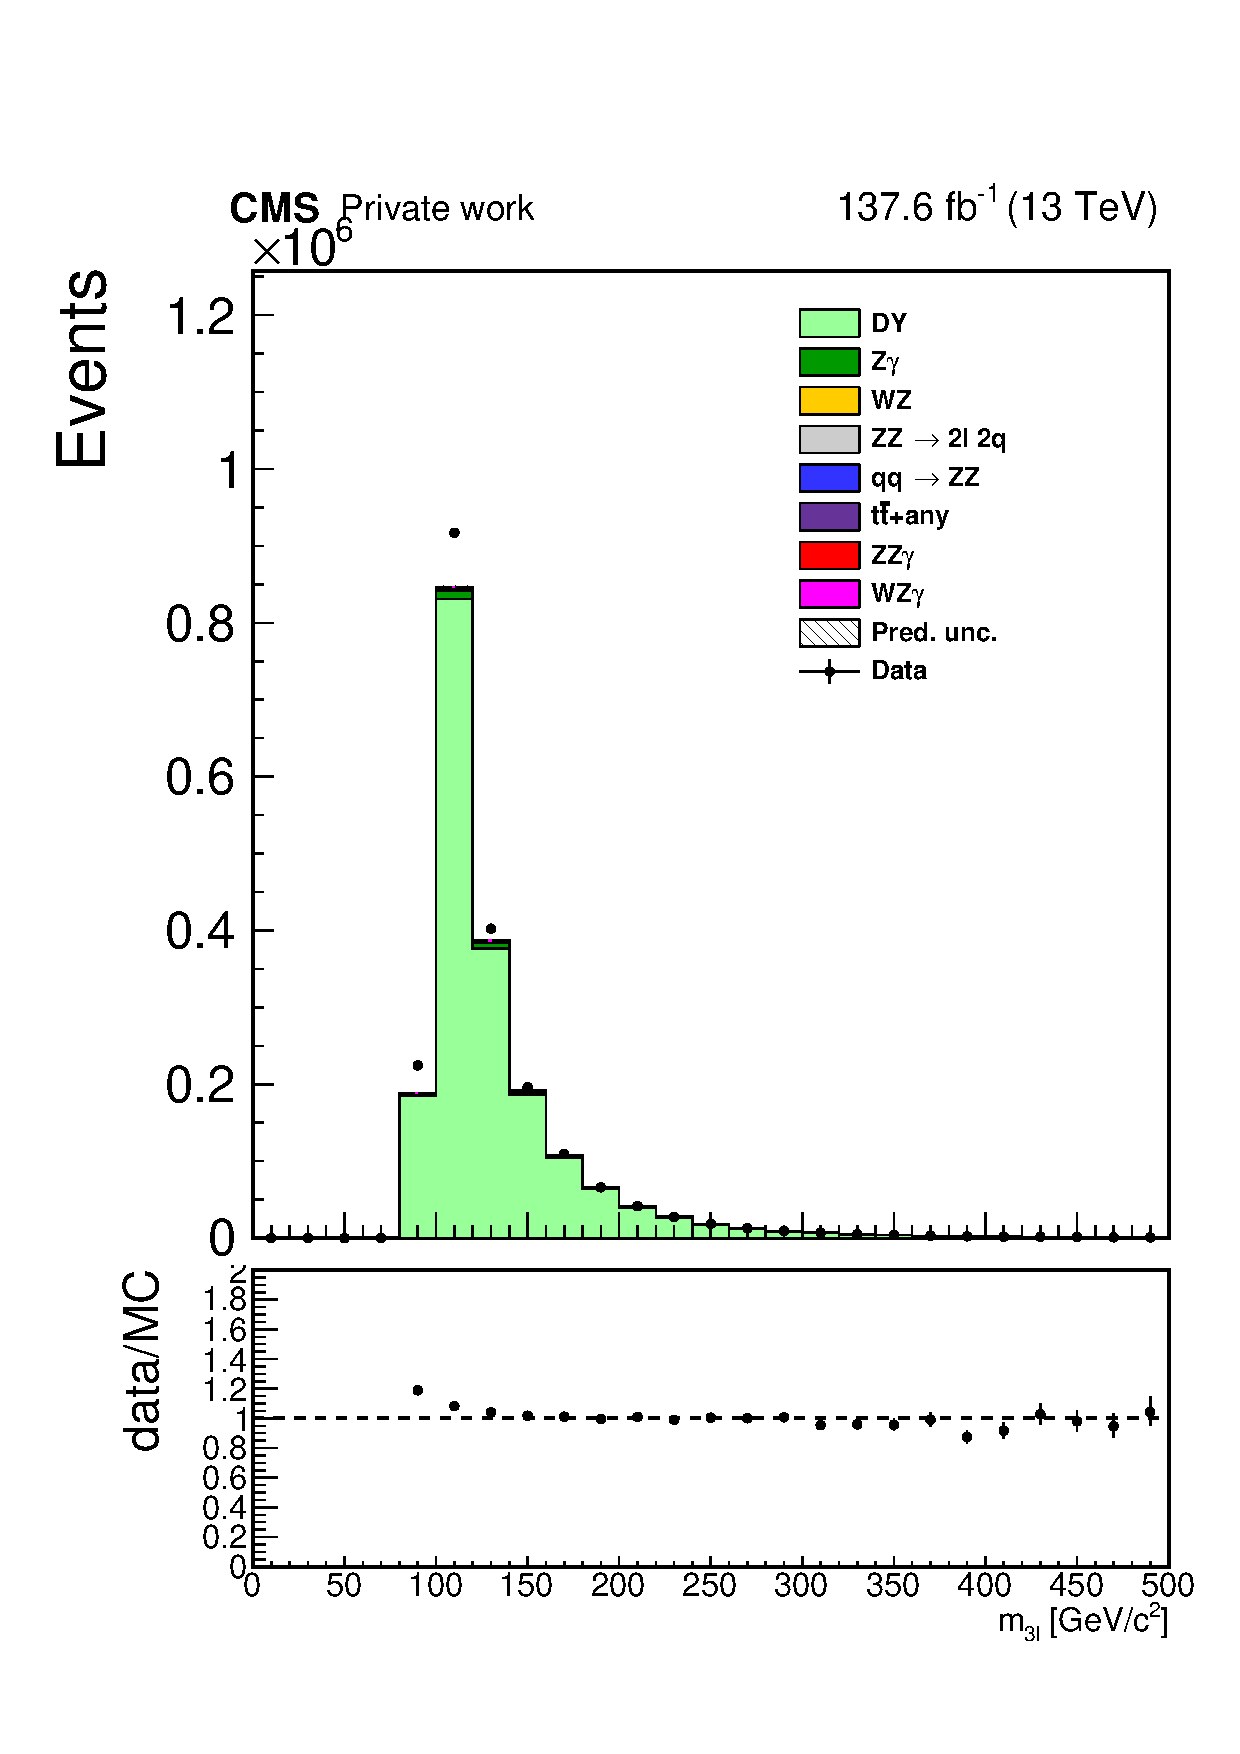
\includegraphics[width=.333333333\textwidth]{VVGammaAnalyzer/Run2/fullMC/CRLFR/ZL_mass_pow.pdf}}%
  \subfigure [$\pt$ of $\Pl^0$] {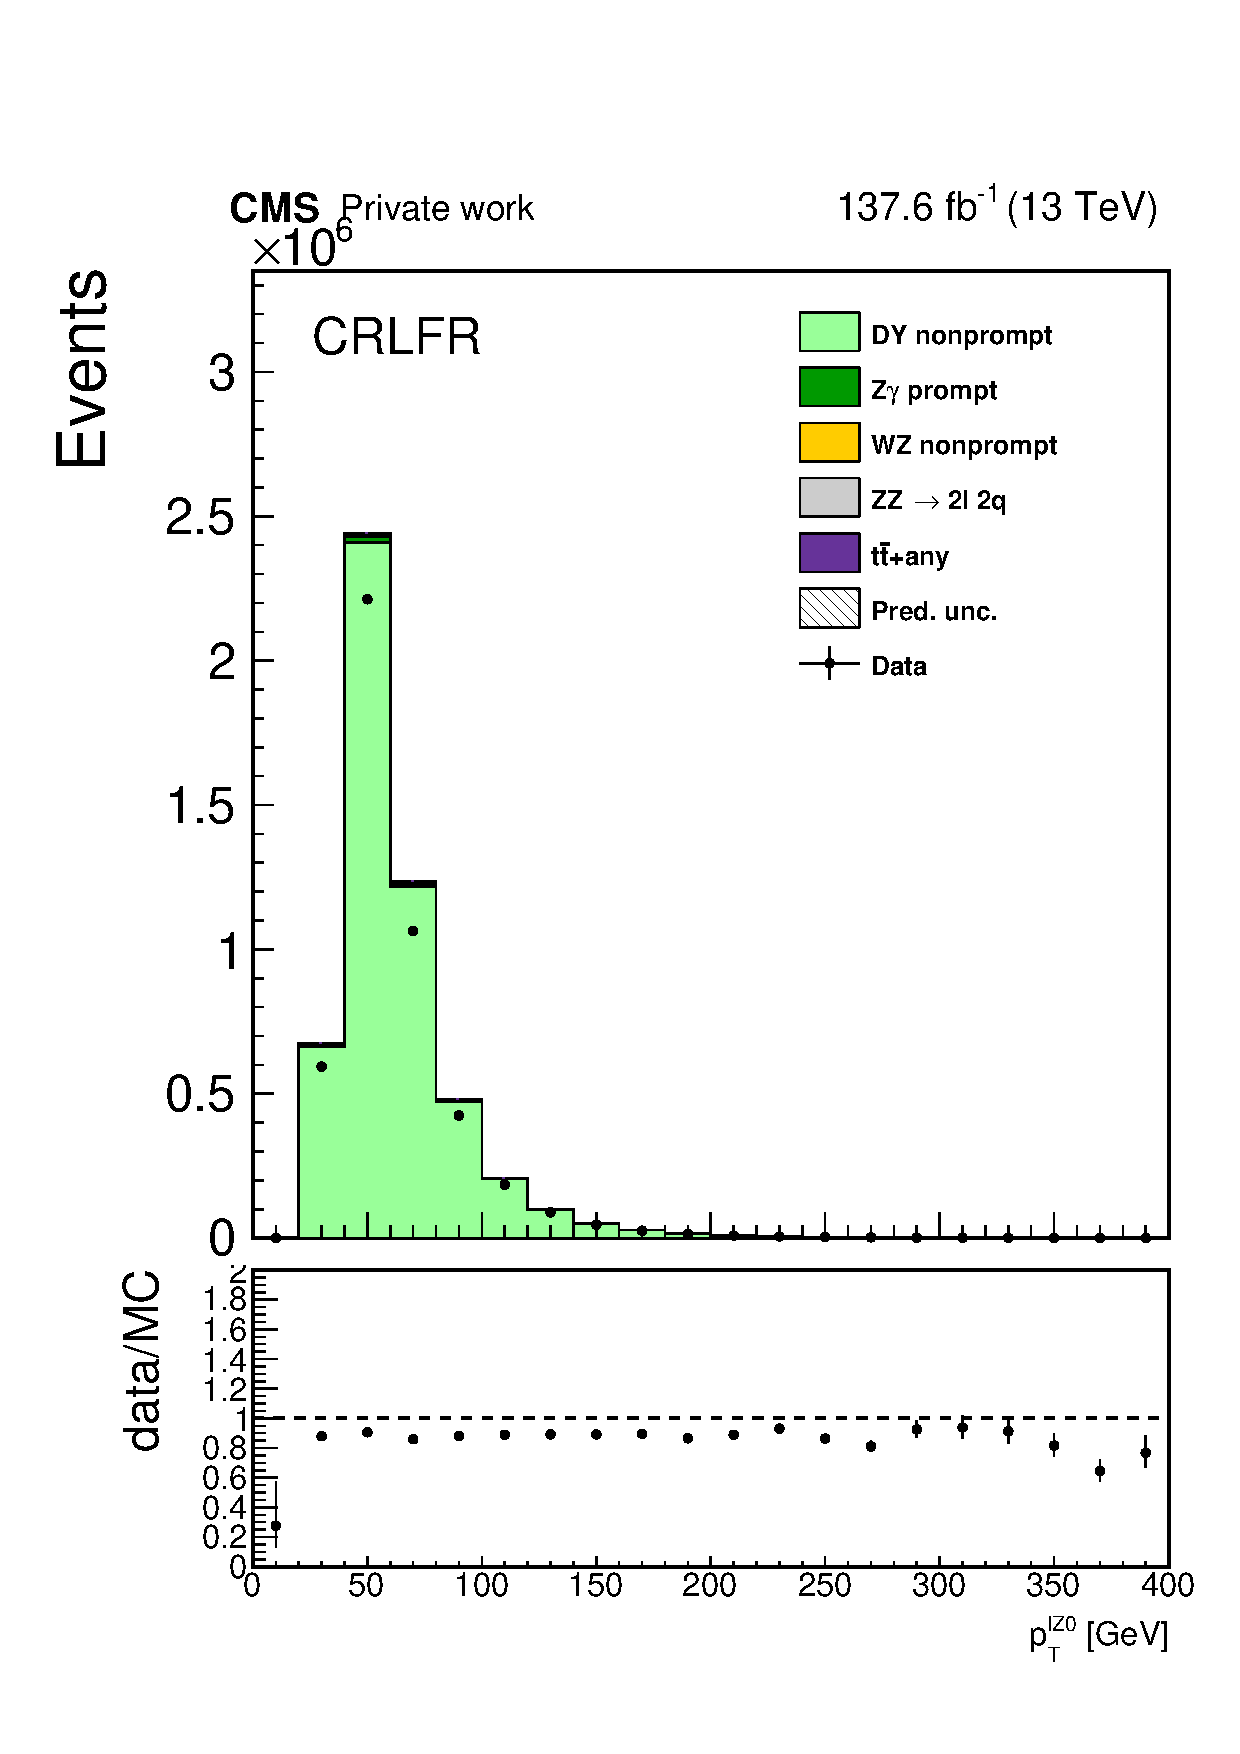
\includegraphics[width=.333333333\textwidth]{VVGammaAnalyzer/Run2/fullMC/CRLFR/Z_l0_pt_pow.pdf}}%
  \subfigure [Number of $\PGg^{\rm kinematic}$] {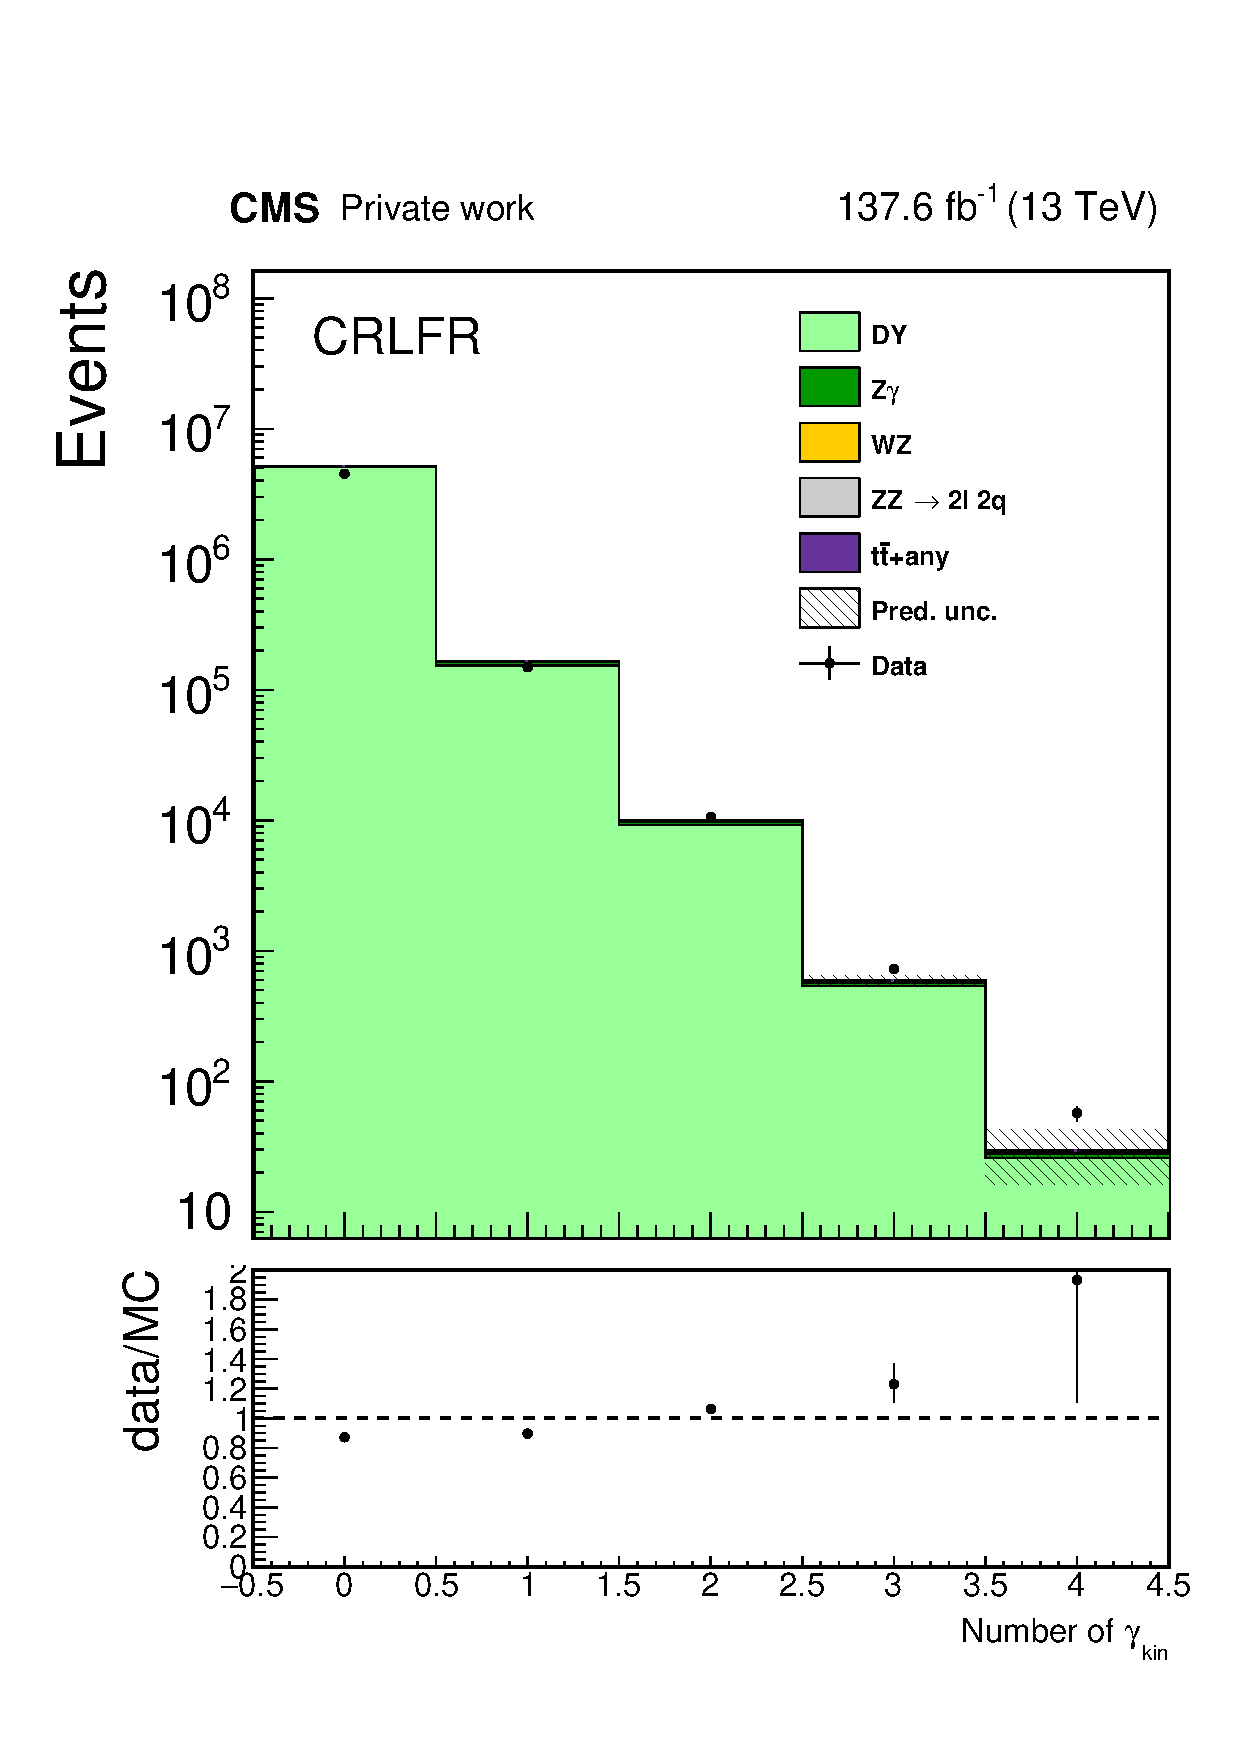
\includegraphics[width=.333333333\textwidth]{VVGammaAnalyzer/Run2/fullMC/CRLFR/kinPh_central_N_pow.pdf}\label{fig:CRLFR_inclusive_kin_N}}
  \caption{Invariant mass of the three lepton system (left),
    transverse momentum of the leading lepton from the Z candidate (centre)
    and number of photon passing the kinematic selection (right)
    in the fake rate measurement region $\PZ+{\rm L}$, integrated on the whole \Run2 period.
    }
  \label{fig:CRLFR_inclusive}
\end{figure}

\begin{figure}
  \centering
  \subfigure [$\pt   $ of $\PGg^{\rm fail}$] {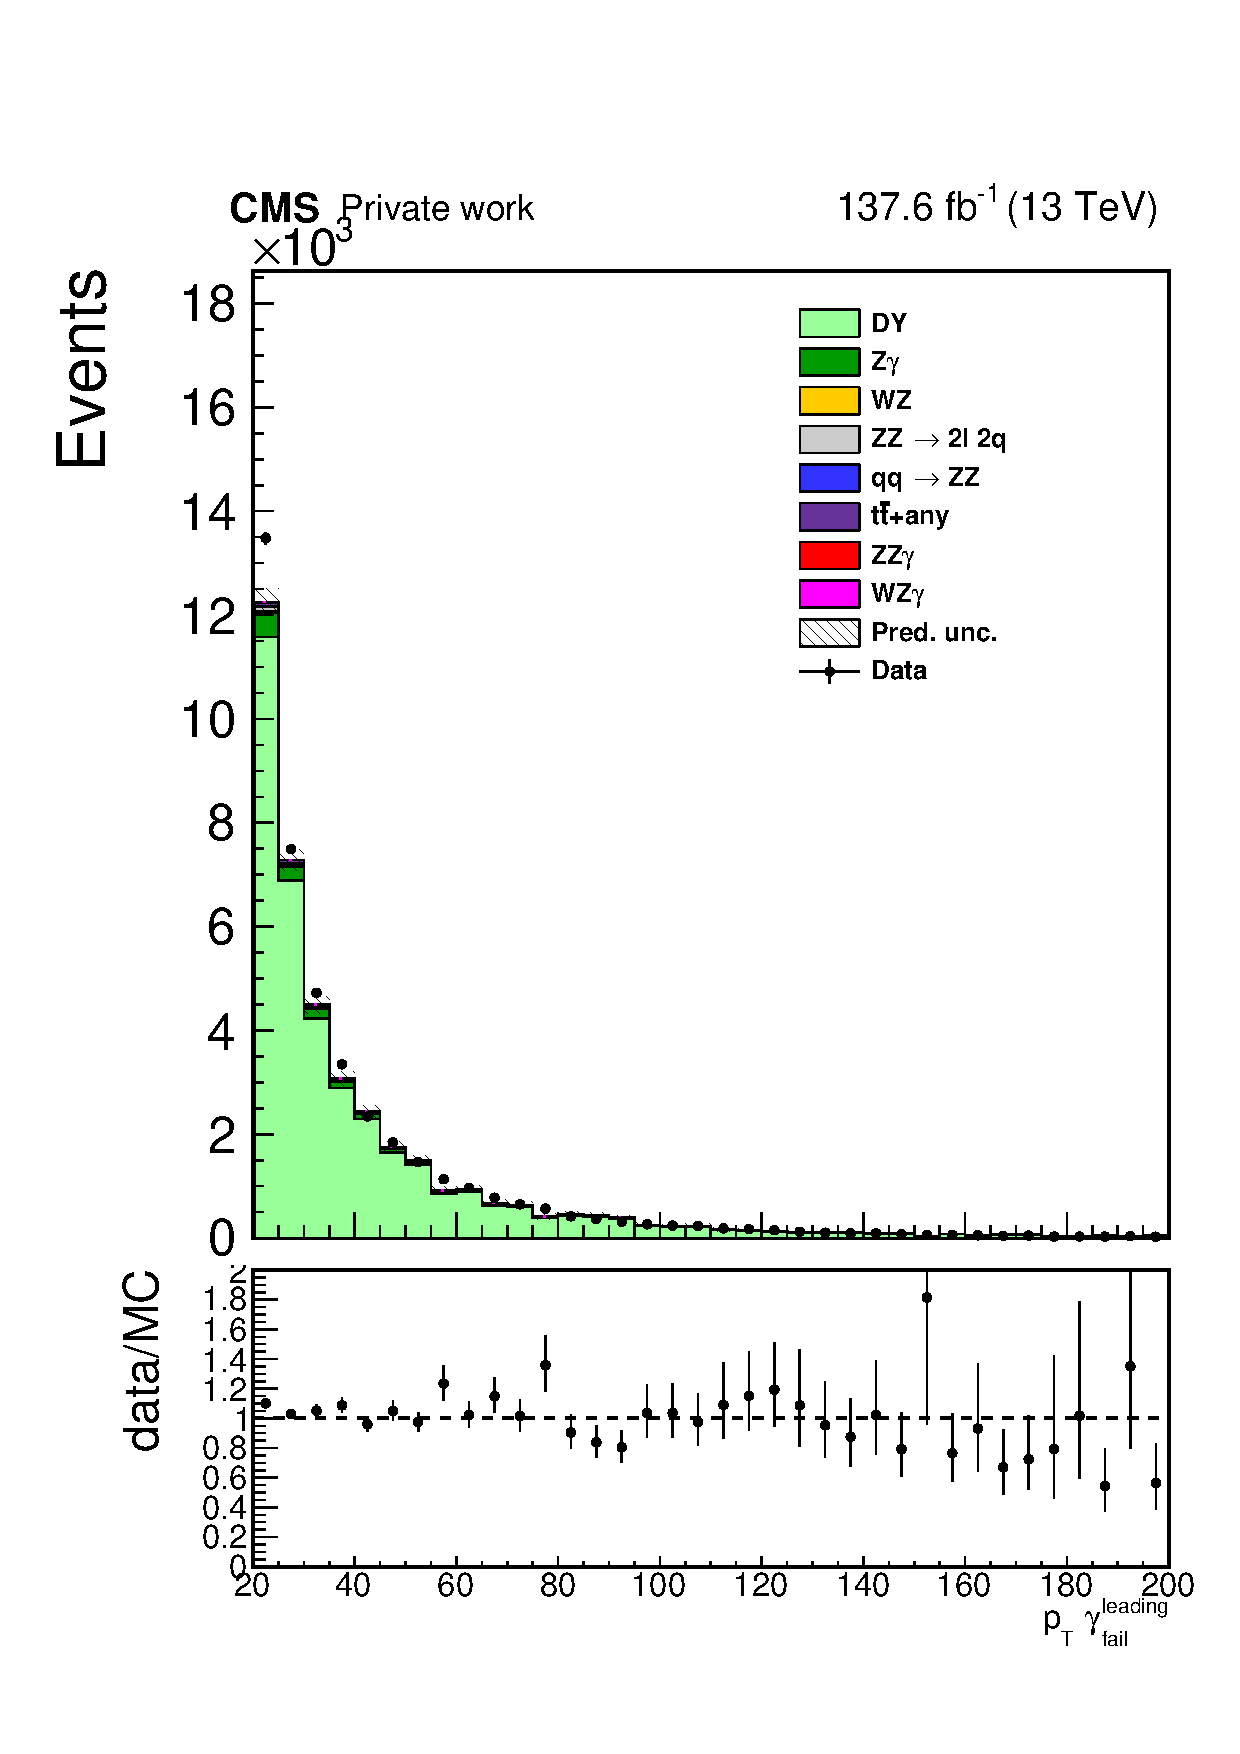
\includegraphics[width=.333333333\textwidth]{VVGammaAnalyzer/Run2/fullMC/CRLFR/lead_fail_pt_fine_pow.pdf}}%
  \subfigure [$|\eta|$ of $\PGg^{\rm fail}$] {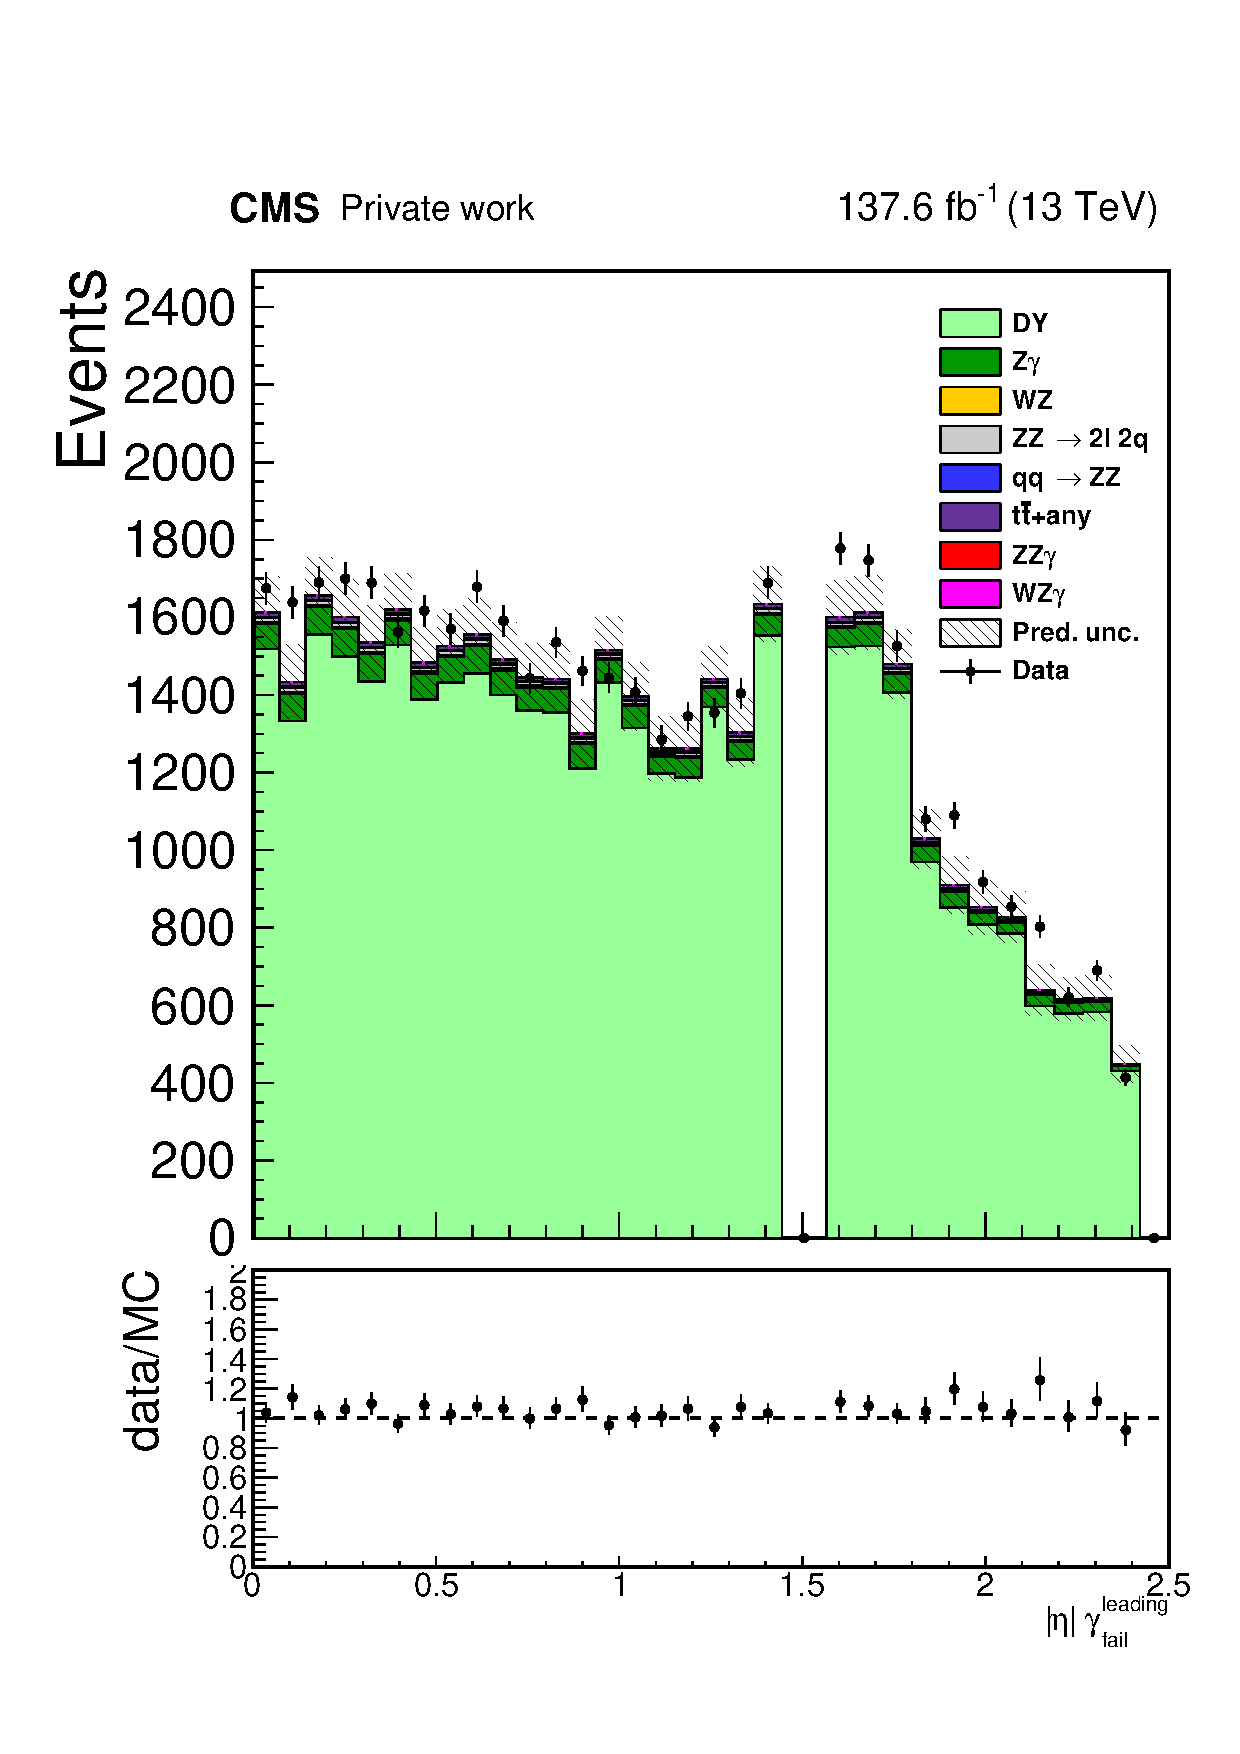
\includegraphics[width=.333333333\textwidth]{VVGammaAnalyzer/Run2/fullMC/CRLFR/lead_fail_aeta_fine_pow.pdf}}%
  \subfigure [$\sieie$ of $\PGg^{\rm fail}$] {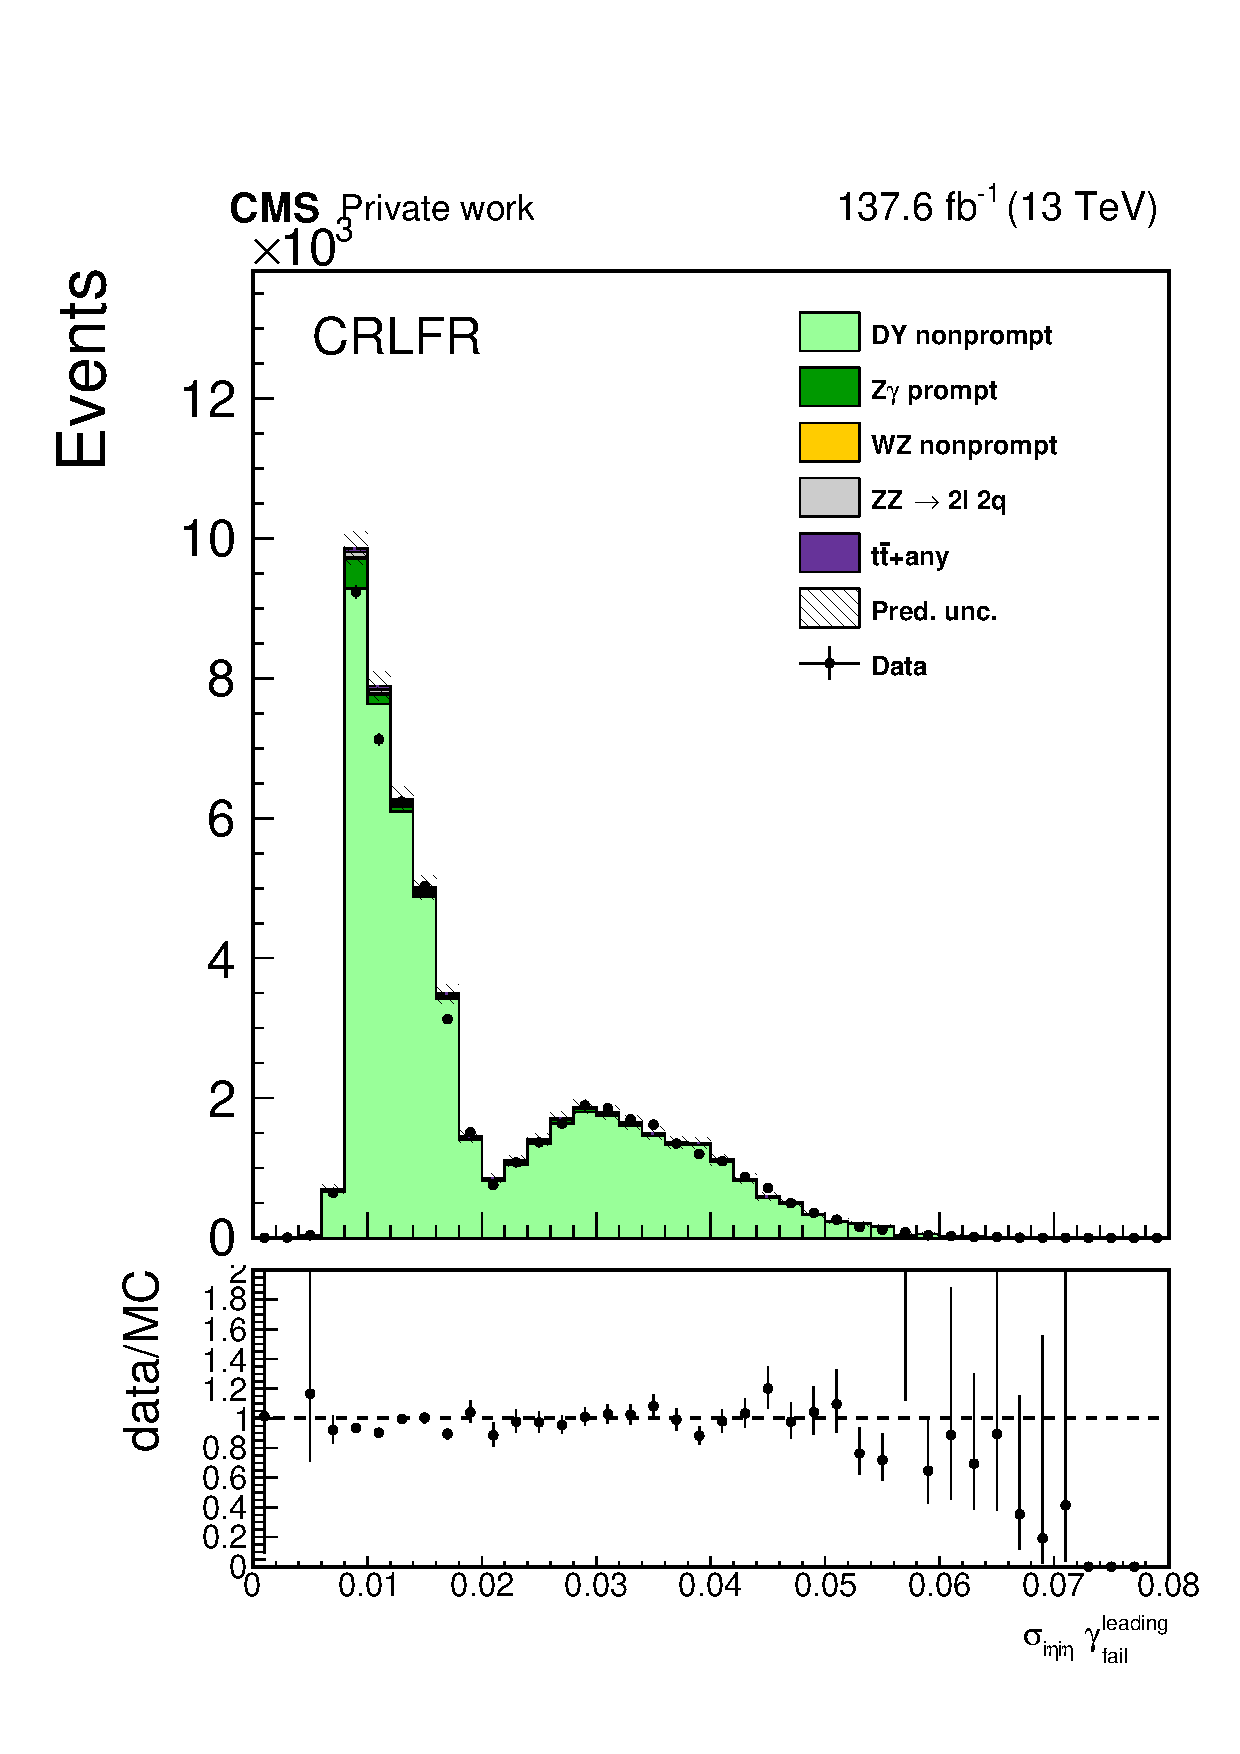
\includegraphics[width=.333333333\textwidth]{VVGammaAnalyzer/Run2/fullMC/CRLFR/lead_fail_sieie_pow.pdf}}
  \caption{Transverse momentum, pseudorapidity and \sieie of photons
    passing the loose criterion (VeryLoose ID) but failing the tight selection (Loose working point of the cut-based ID)
    in the fake rate measurement region, integrated on the whole \Run2 period.}
  \label{fig:CRLFR_lead_fail}
\end{figure}

\begin{figure}
  \centering
  \subfigure [$\pt   $ of $\PGg^{\rm pass}$] {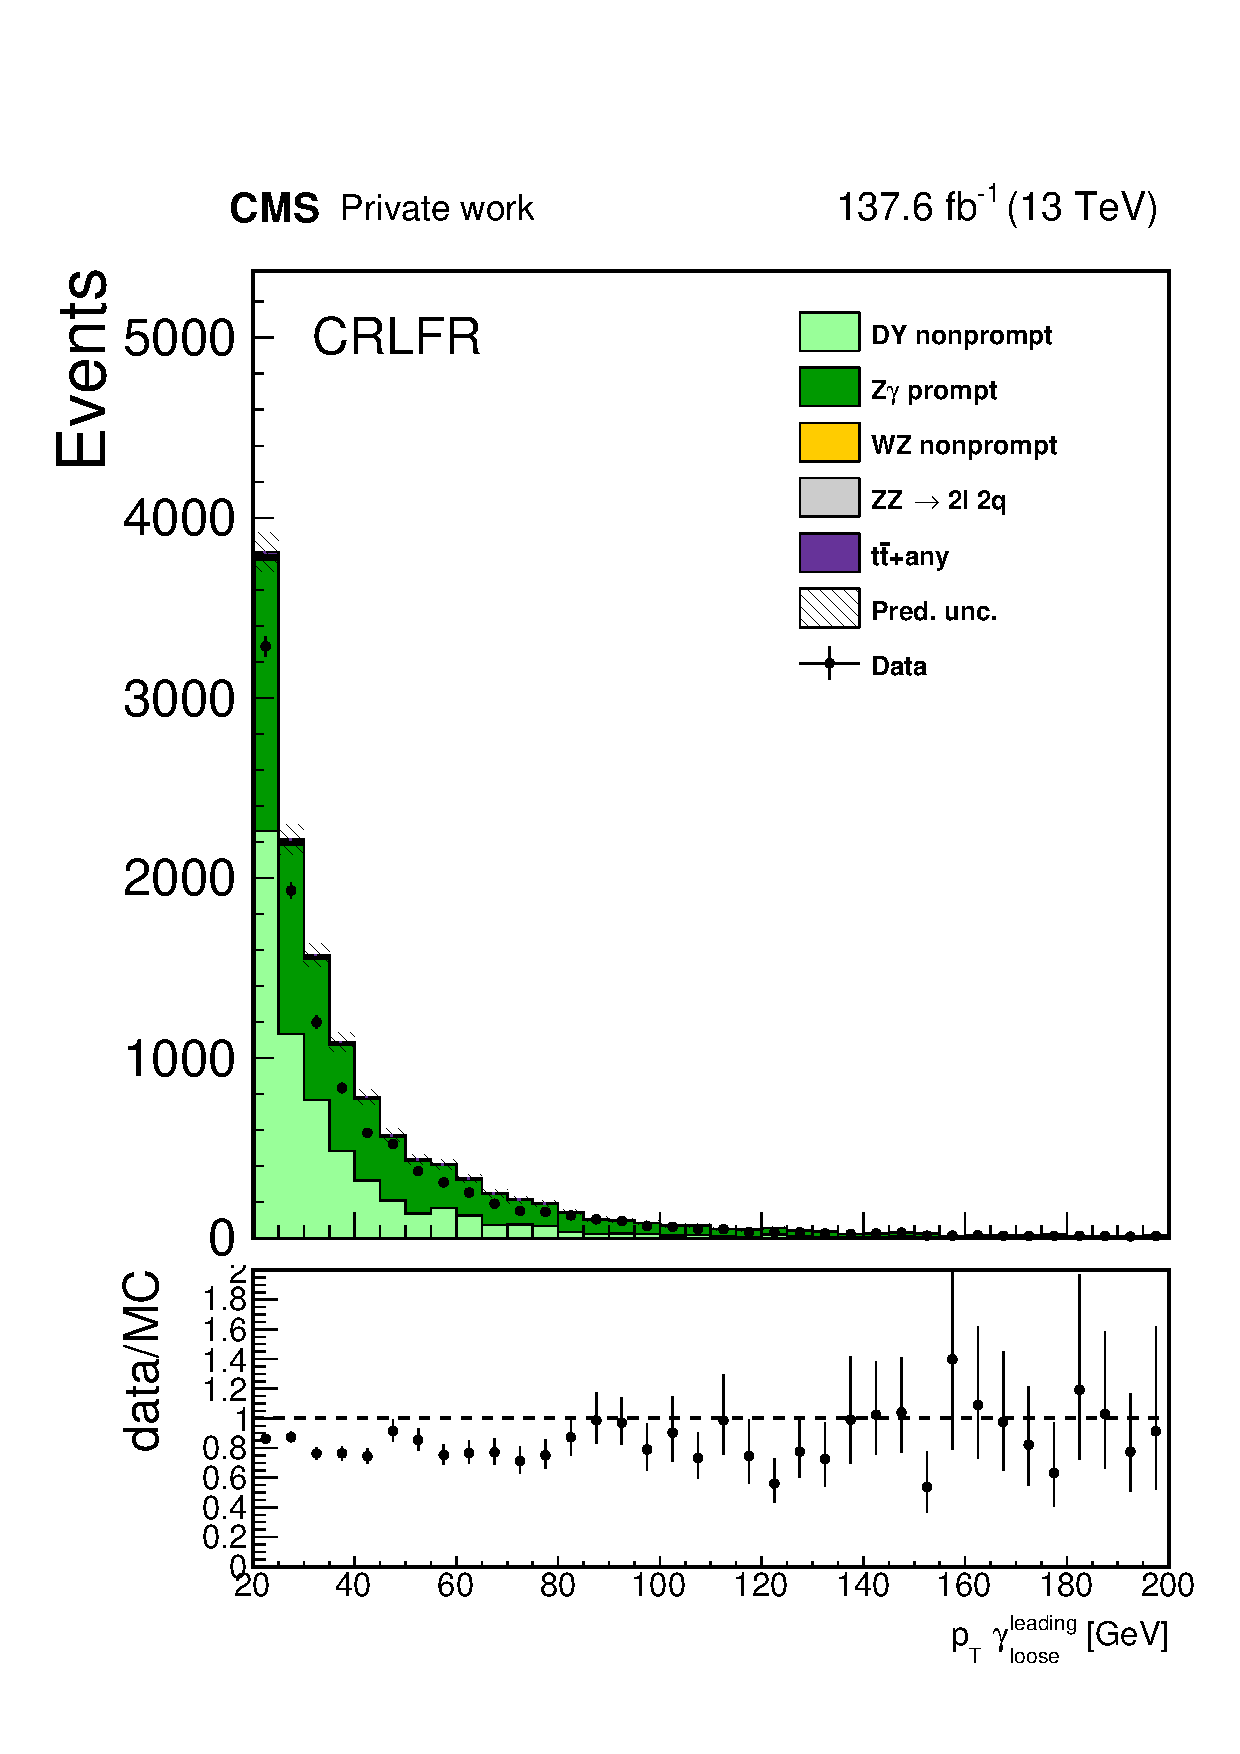
\includegraphics[width=.333333333\textwidth]{VVGammaAnalyzer/Run2/fullMC/CRLFR/lead_loose_pt_fine_pow.pdf}}%
  \subfigure [$|\eta|$ of $\PGg^{\rm pass}$] {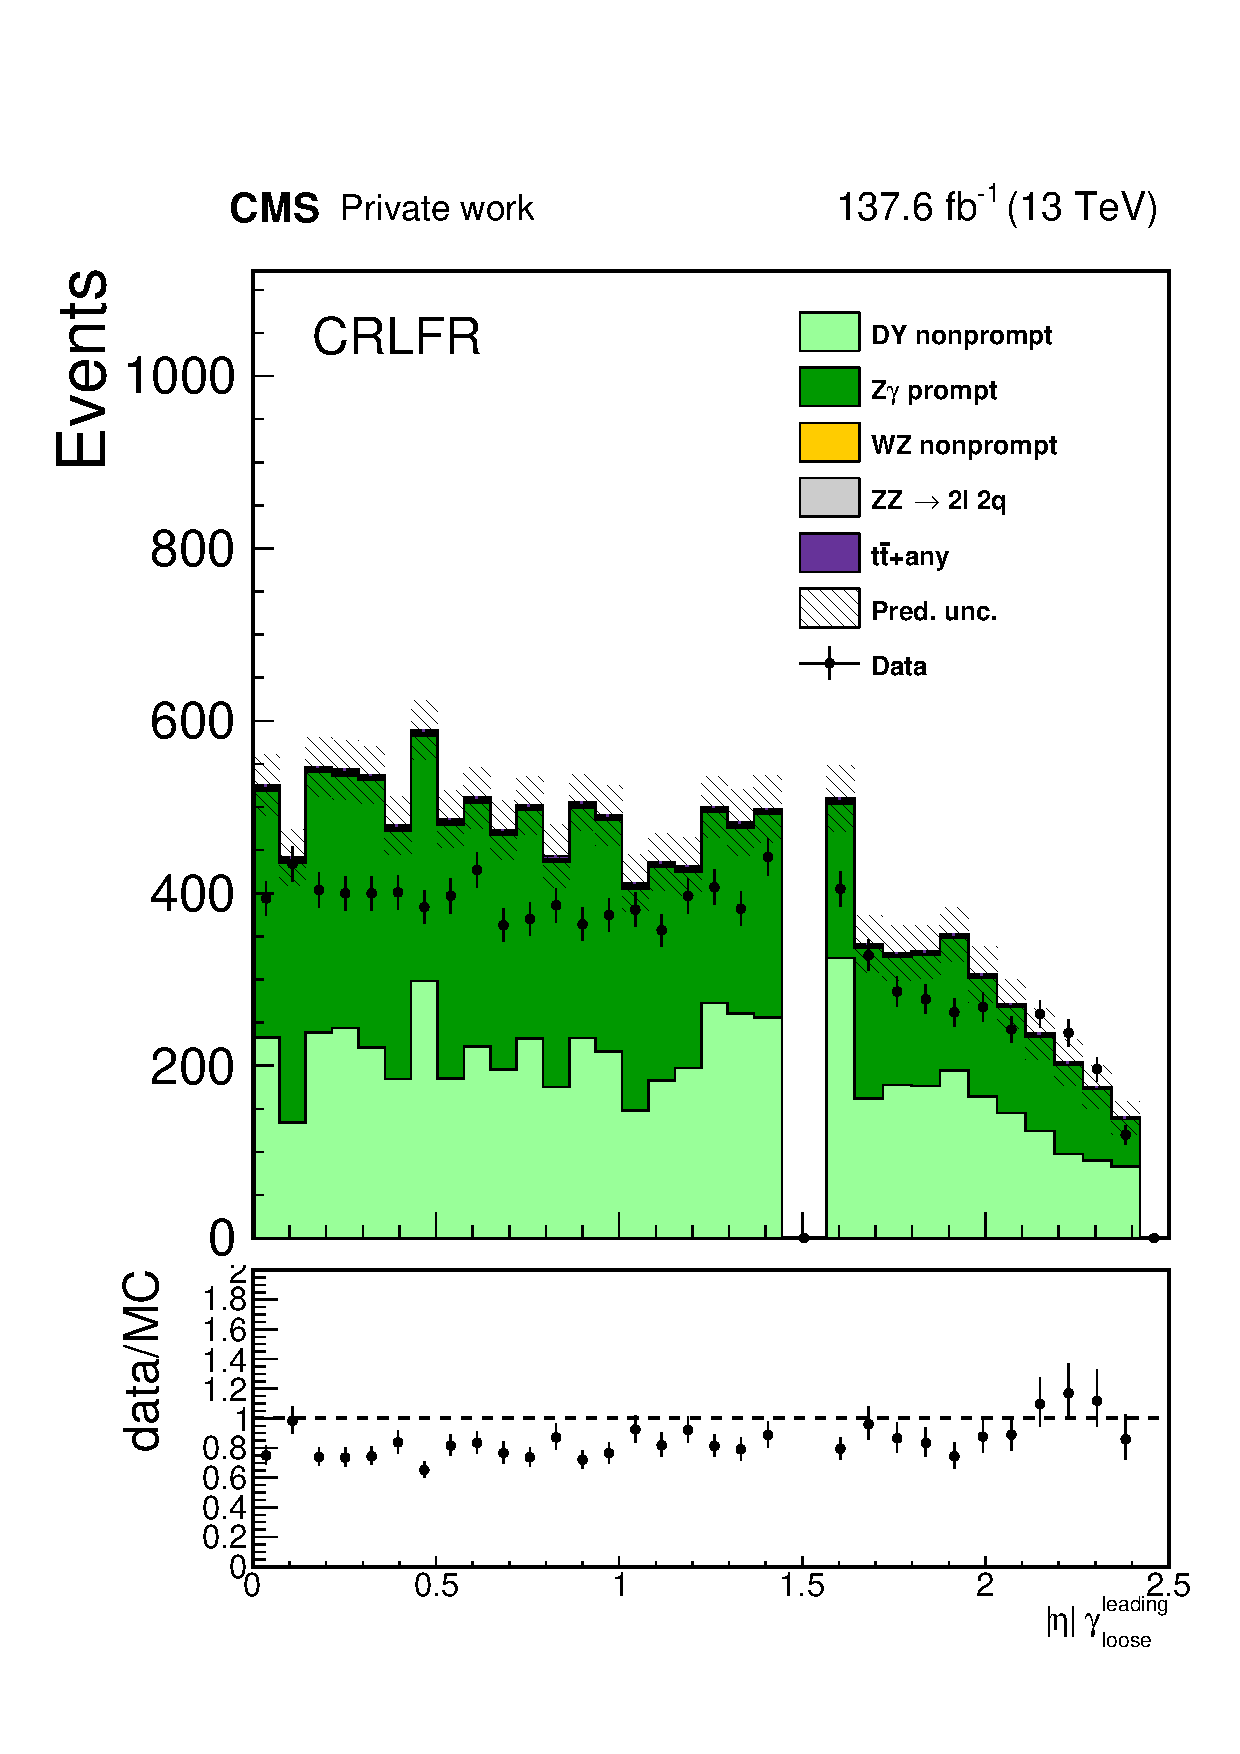
\includegraphics[width=.333333333\textwidth]{VVGammaAnalyzer/Run2/fullMC/CRLFR/lead_loose_aeta_fine_pow.pdf}}%
  \subfigure [$\sieie$ of $\PGg^{\rm pass}$] {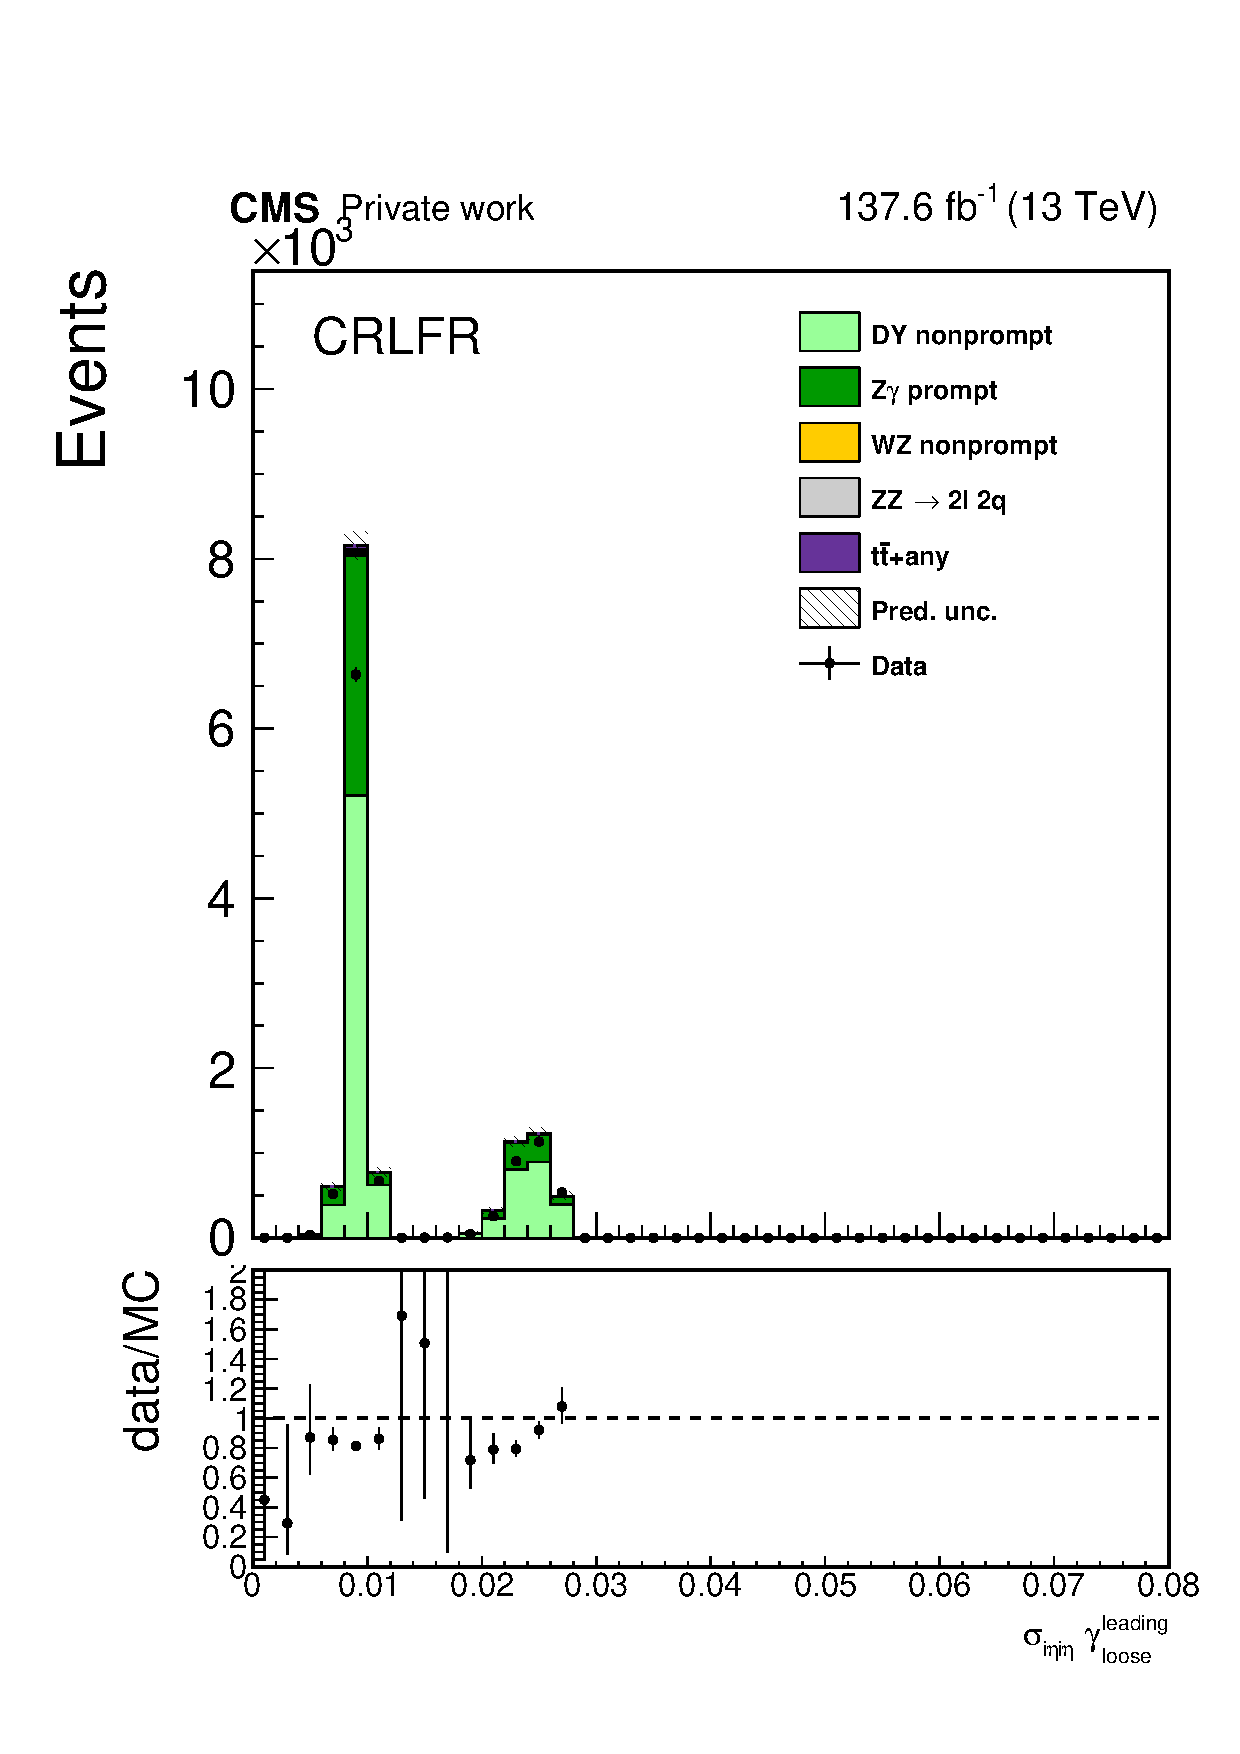
\includegraphics[width=.333333333\textwidth]{VVGammaAnalyzer/Run2/fullMC/CRLFR/lead_loose_sieie_pow.pdf}}
  \caption{Transverse momentum, pseudorapidity and \sieie of photons
    passing the tight selection (Loose working point of the cut-based ID)
    in the fake rate measurement region, integrated on the whole \Run2 period.}
  \label{fig:CRLFR_lead_pass}
\end{figure}

The fake rate is then measured as the ratio of events in which the photon passes also the tight selection (the Loose working point of the cut-based ID)
to the total.
This measurement is done separately for endcap and barrel, for several bins of \pt (Figure \ref{fig:phFR_VLtoL}).

\begin{figure}
\subfigure [2016preVFP ] {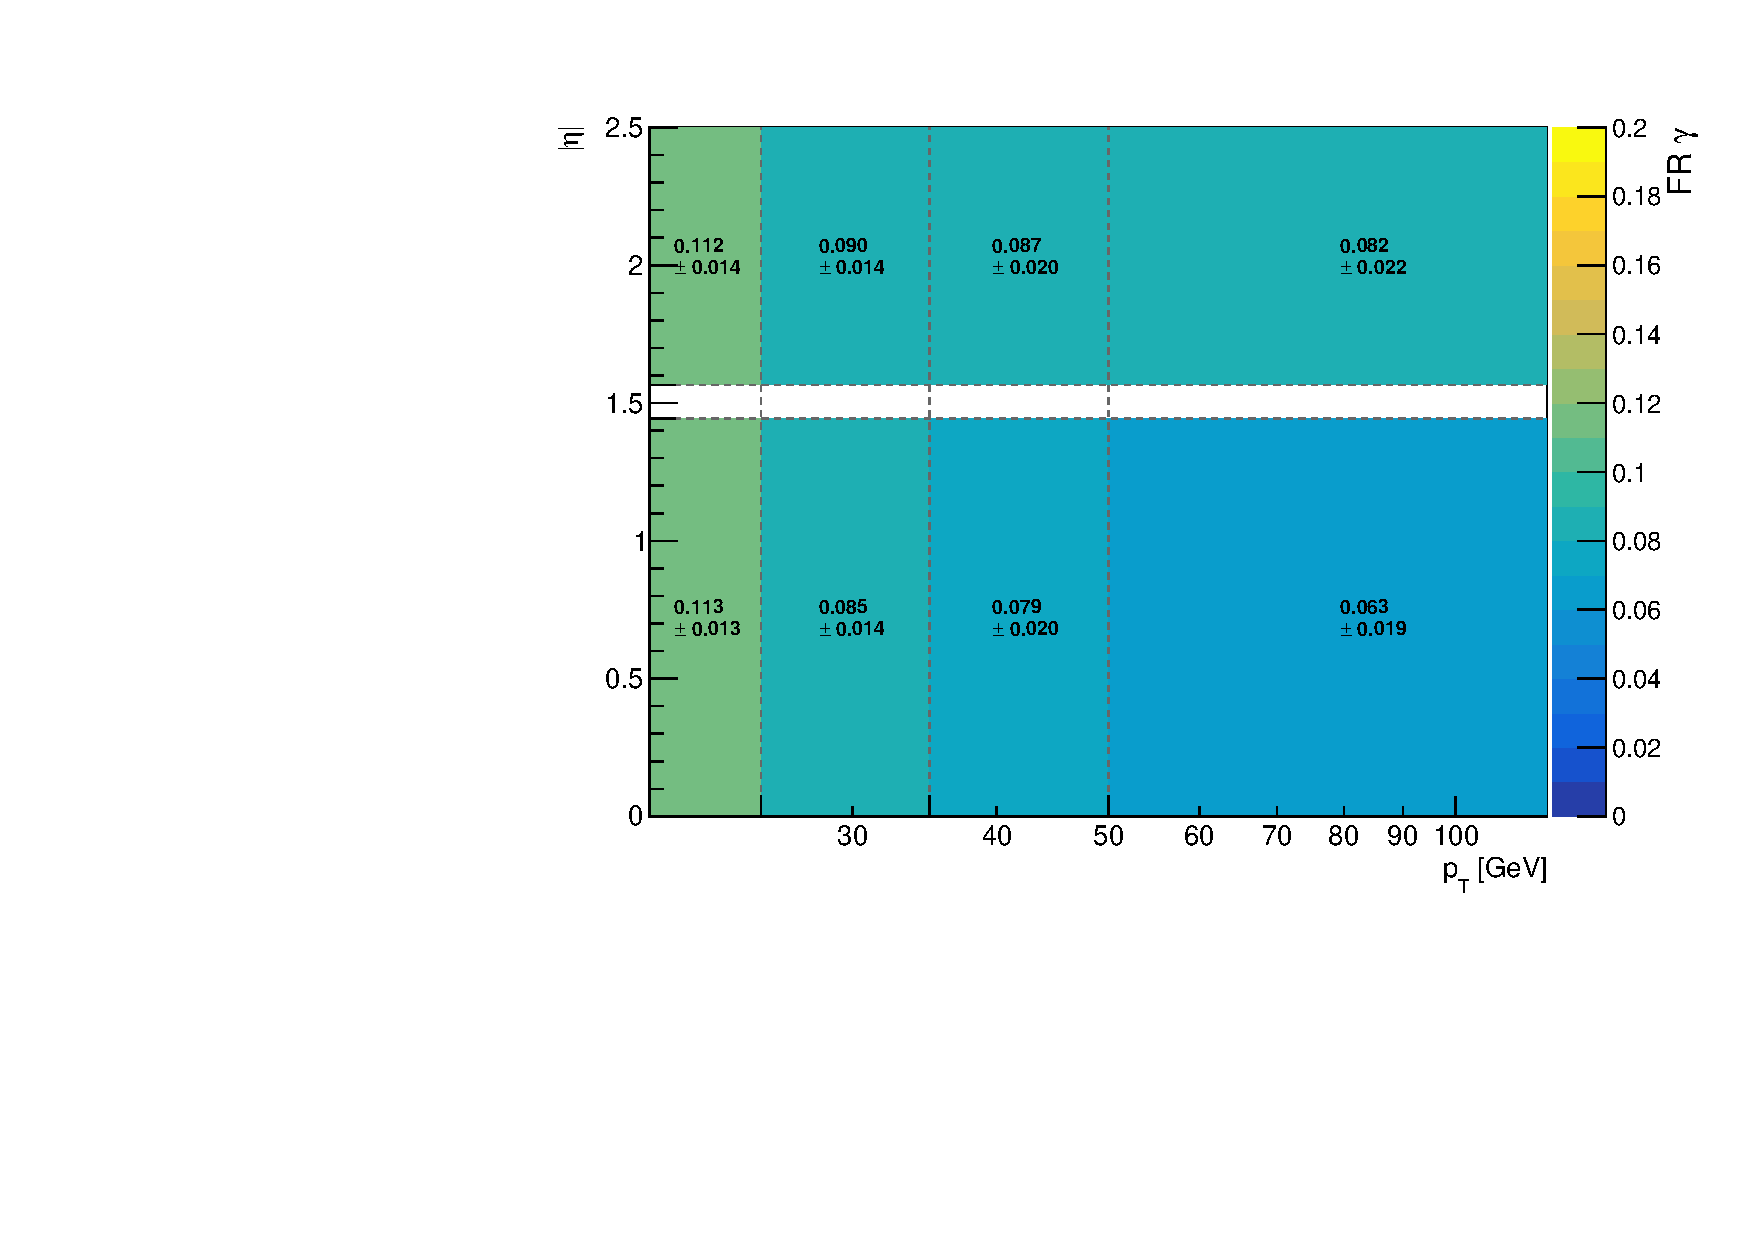
\includegraphics[width=.5\textwidth]{Figures/PhFR/FR_VLtoL_pt-aeta_data-ZGToLLG_2016preVFP.pdf}}%
\subfigure [2016postVFP] {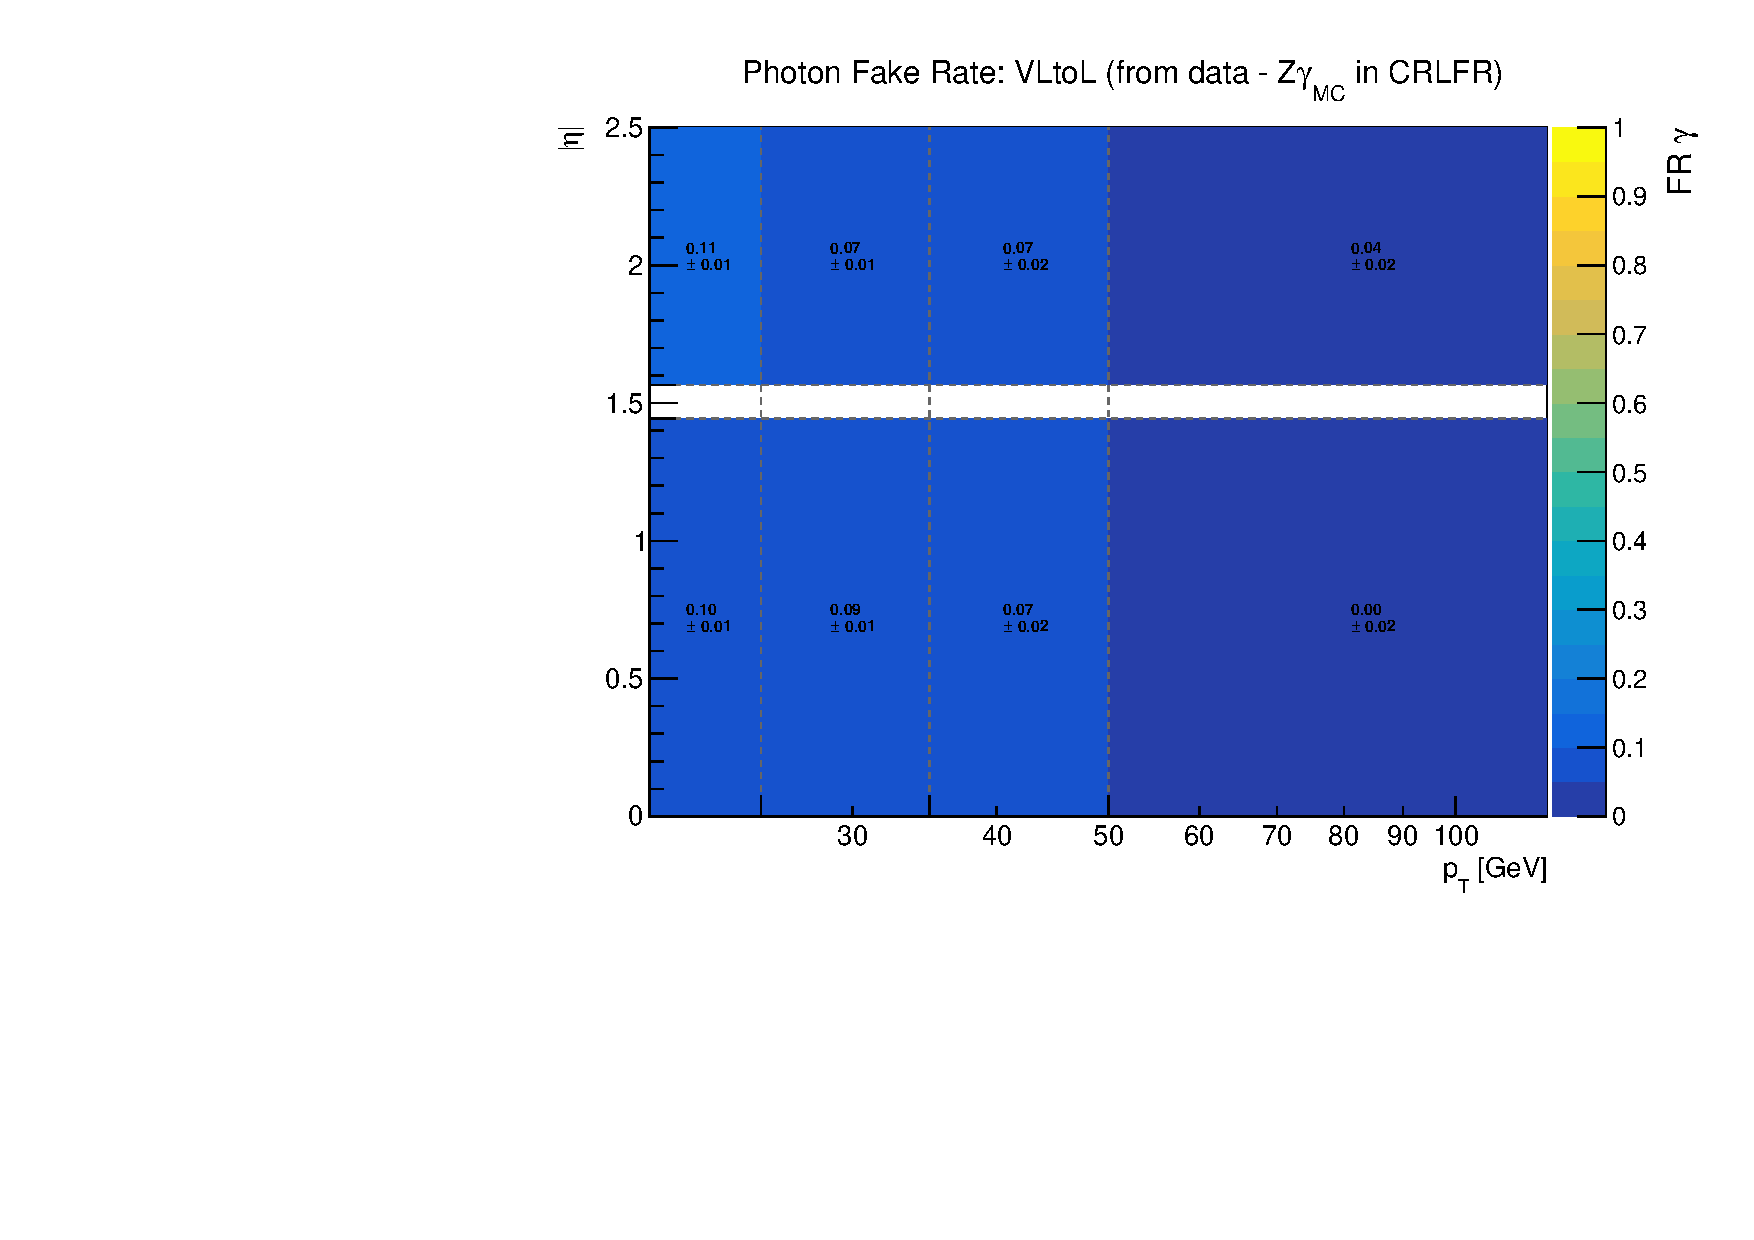
\includegraphics[width=.5\textwidth]{Figures/PhFR/FR_VLtoL_pt-aeta_data-ZGToLLG_2016postVFP.pdf}}\\
\subfigure [2017]        {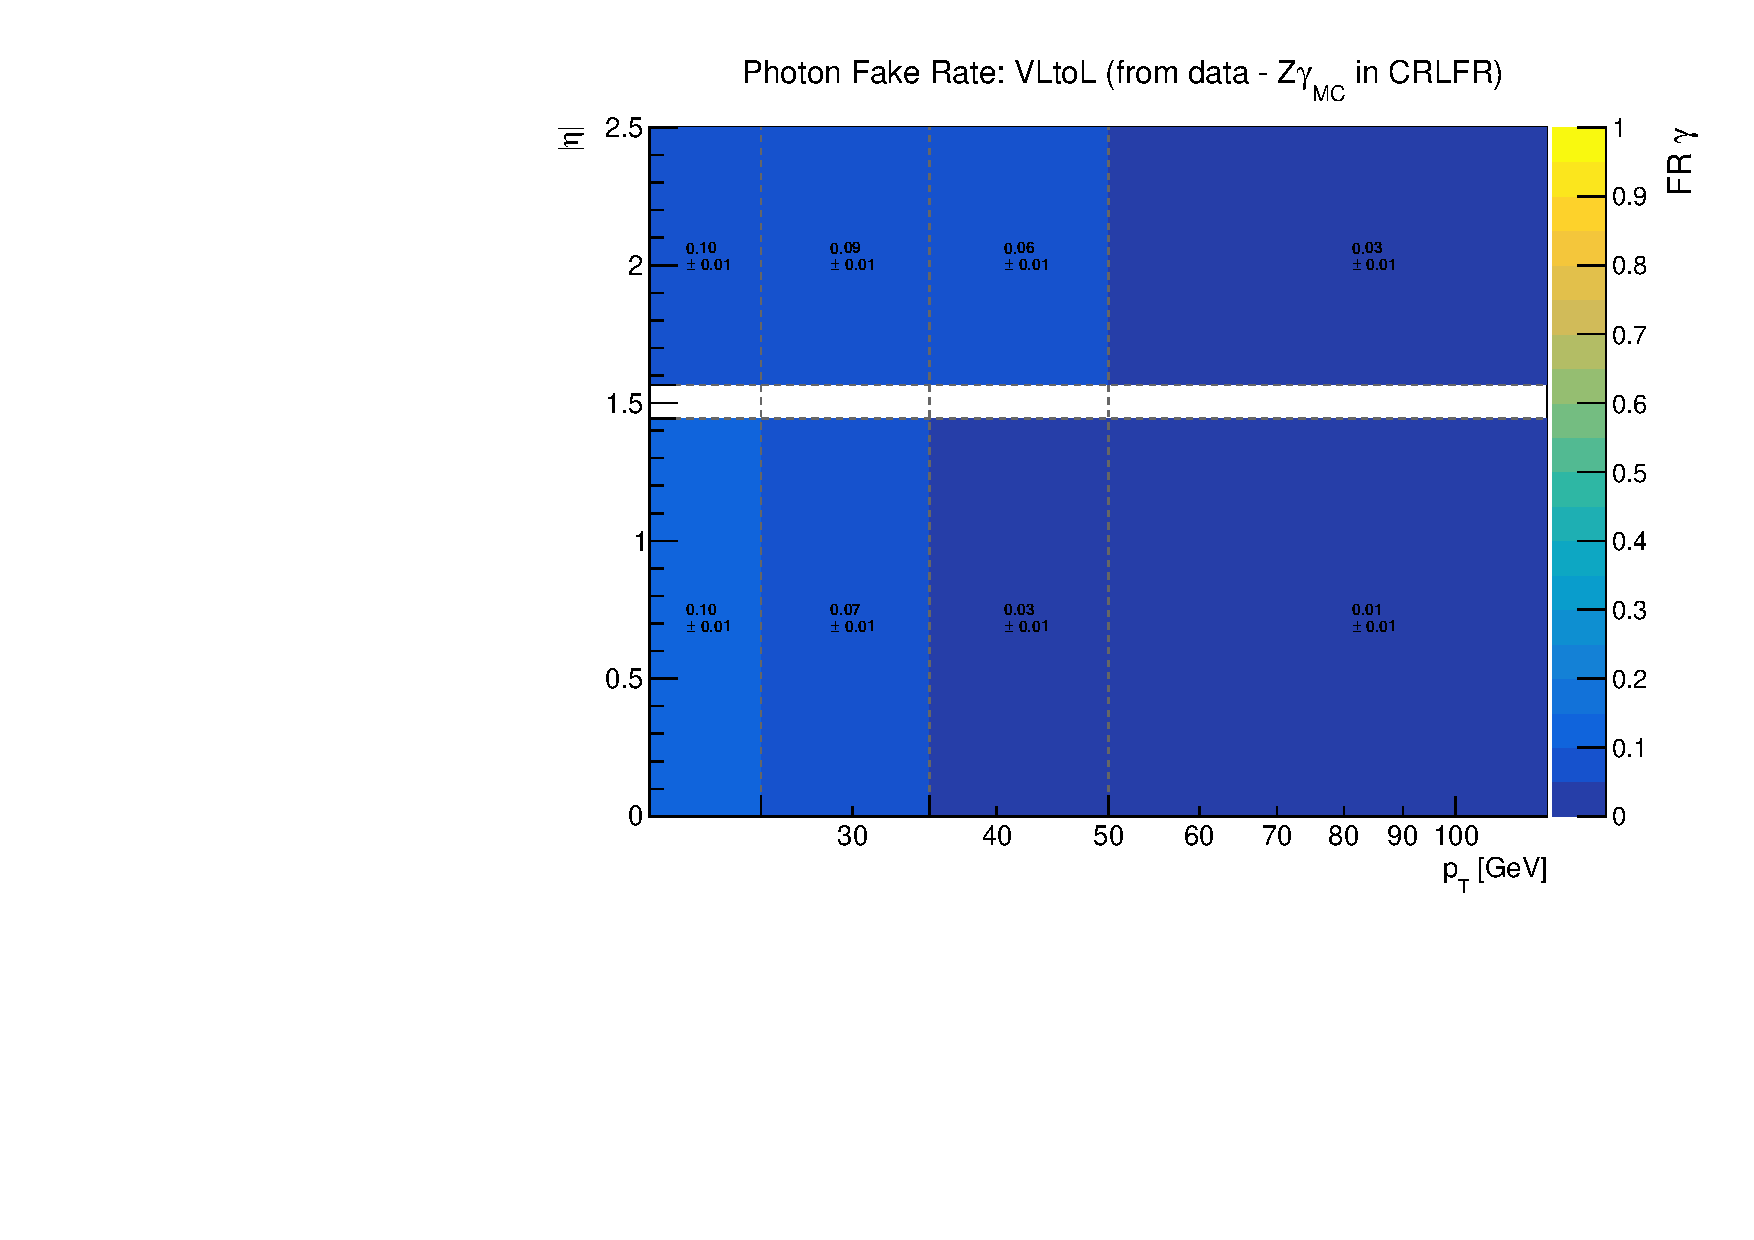
\includegraphics[width=.5\textwidth]{Figures/PhFR/FR_VLtoL_pt-aeta_data-ZGToLLG_2017.pdf}}%
\subfigure [2018]        {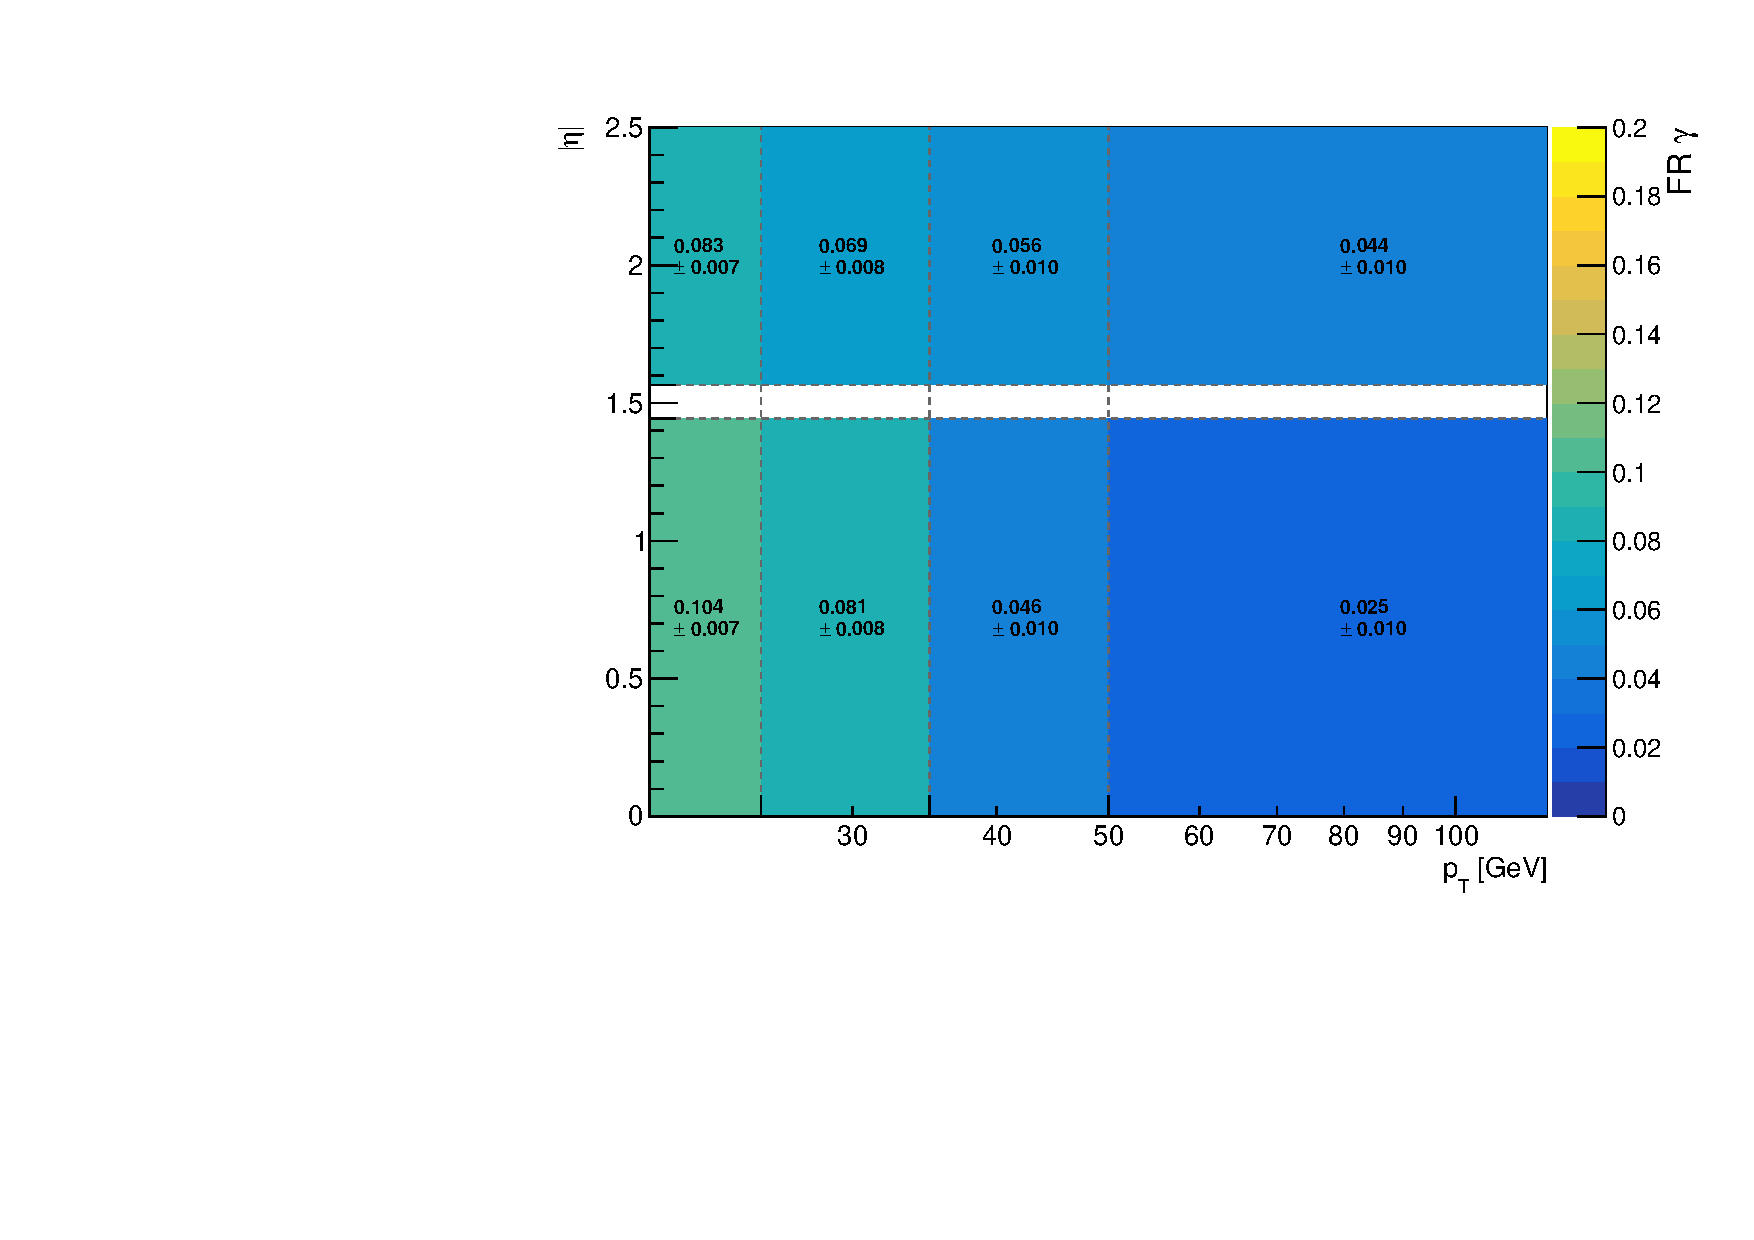
\includegraphics[width=.5\textwidth]{Figures/PhFR/FR_VLtoL_pt-aeta_data-ZGToLLG_2018.pdf}}
\caption{Photon non-prompt rate as measured in data (with prompt $Z\gamma$ subtraction) using the cut-based ID for the photon.}
\label{fig:phFR_VLtoL}
\end{figure}

To ensure the stability of the measurement against other variables in the event,
additional measurements are carried out in specific sub-regions, and the results compared.
In particular, the effect of the following was studied:
\begin{itemize}
\item The status of the third lepton: whether it passes or fails the tight selection.
  This could bias the measurement if the lepton were a misidentified jet
  and the additional hadronic activity produced an additional \nonprompt photon (Figure~\ref{fig:phFR_PF}).
\item The flavour of the third lepton (Figure~\ref{fig:phFR_em}).
\item The flavour of the lepton pair that constitutes the \PZ boson (Figure~\ref{fig:phFR_2e2m}).
\item The number of additional jets in the event.
\item The distance of the photon from the closest jet in the event.
\end{itemize}

The photon non-prompt rate is assumed to be independent of the flavour of the leptons in the event.
The potential impact on the fake rate caused by \eg differences in the bremsstrahlung emissions between electrons and muons is tested by
deriving it separately for each flavour of the leptons of the Z boson $\Pep\Pem \Pl^\pm$ and $\PGmp\PGmm \Pl^\pm$, as shown in Figure \ref{fig:phFR_2e2m}.

\begin{figure}
\subfigure [$e^+ e^- \ell^\pm$]     {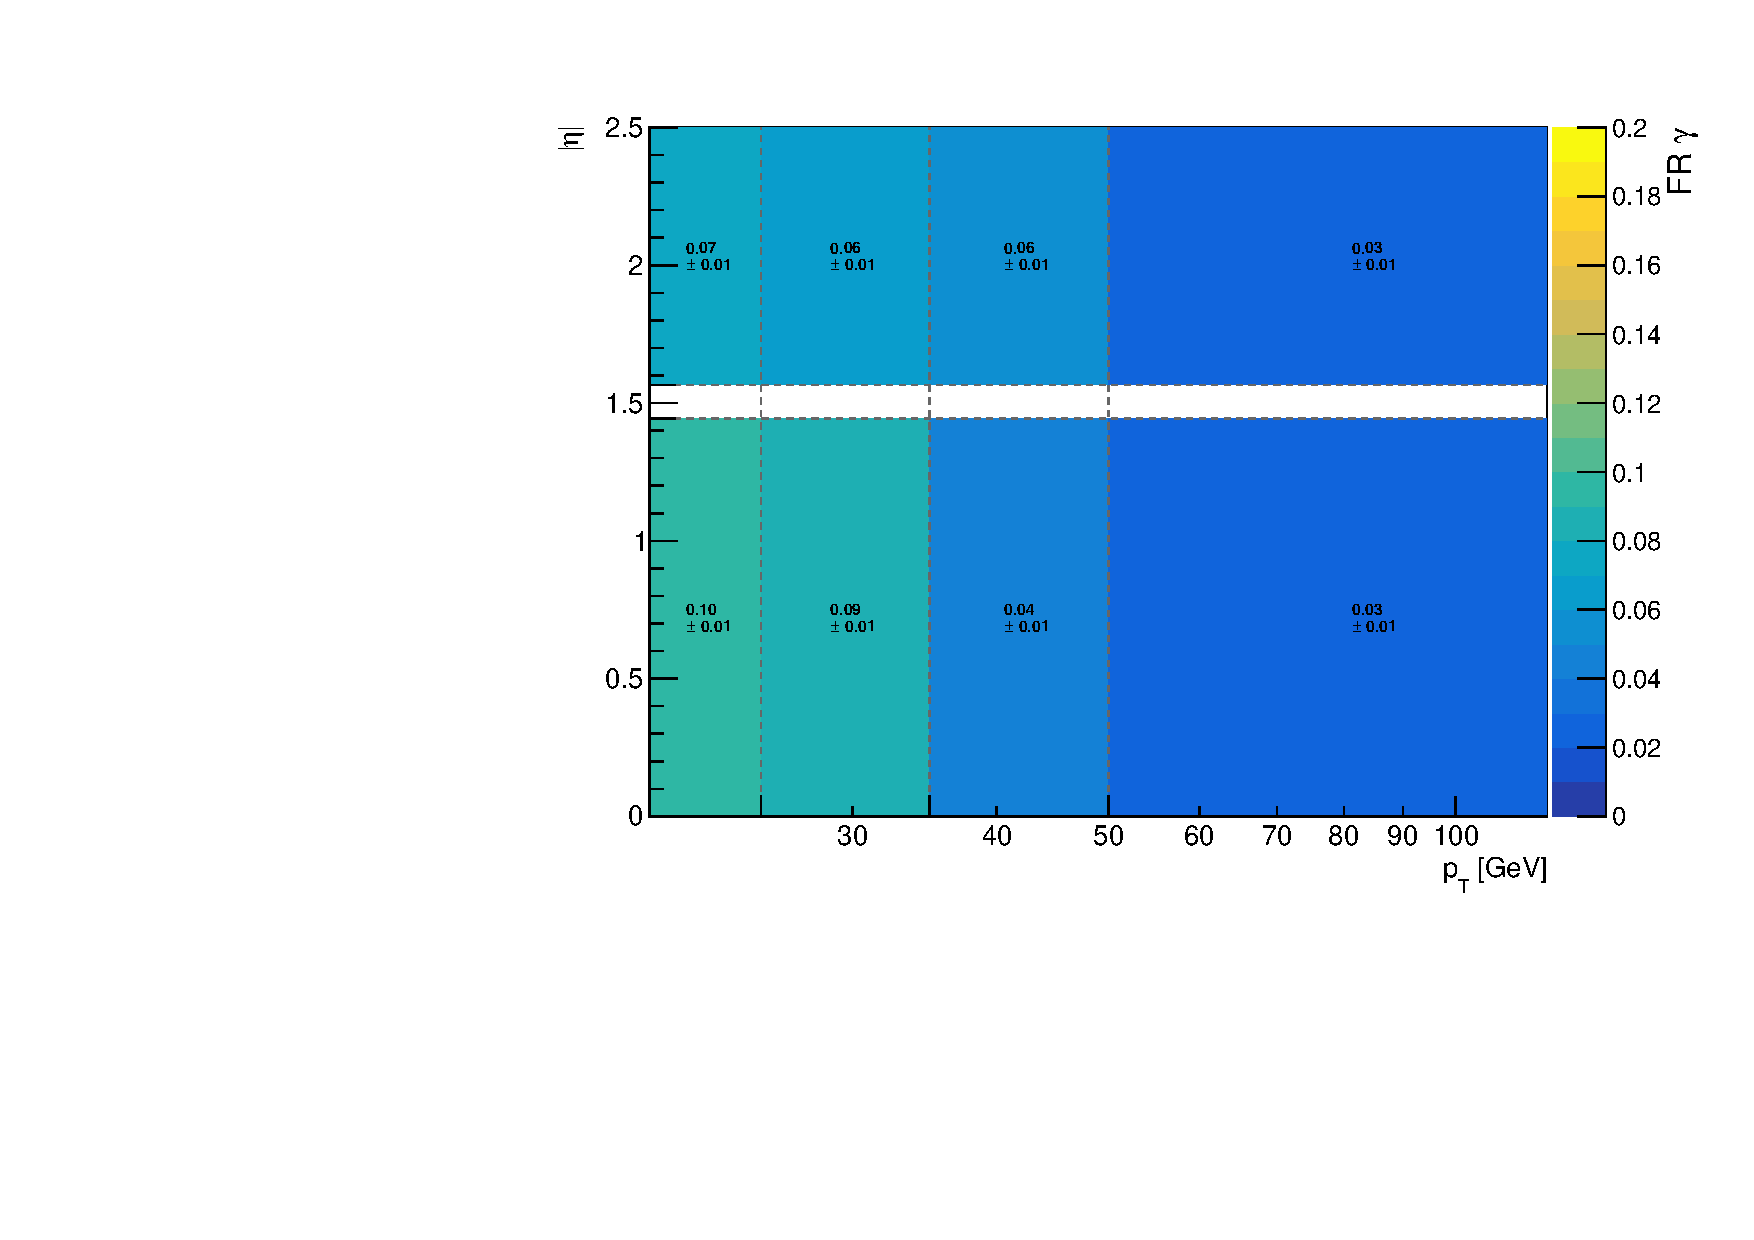
\includegraphics[width=.5\textwidth]{Figures/PhFR/FR_VLtoL_pt-aeta_2e+x_data-ZGToLLG_2018.pdf}}%
\subfigure [$\mu^+ \mu^- \ell^\pm$] {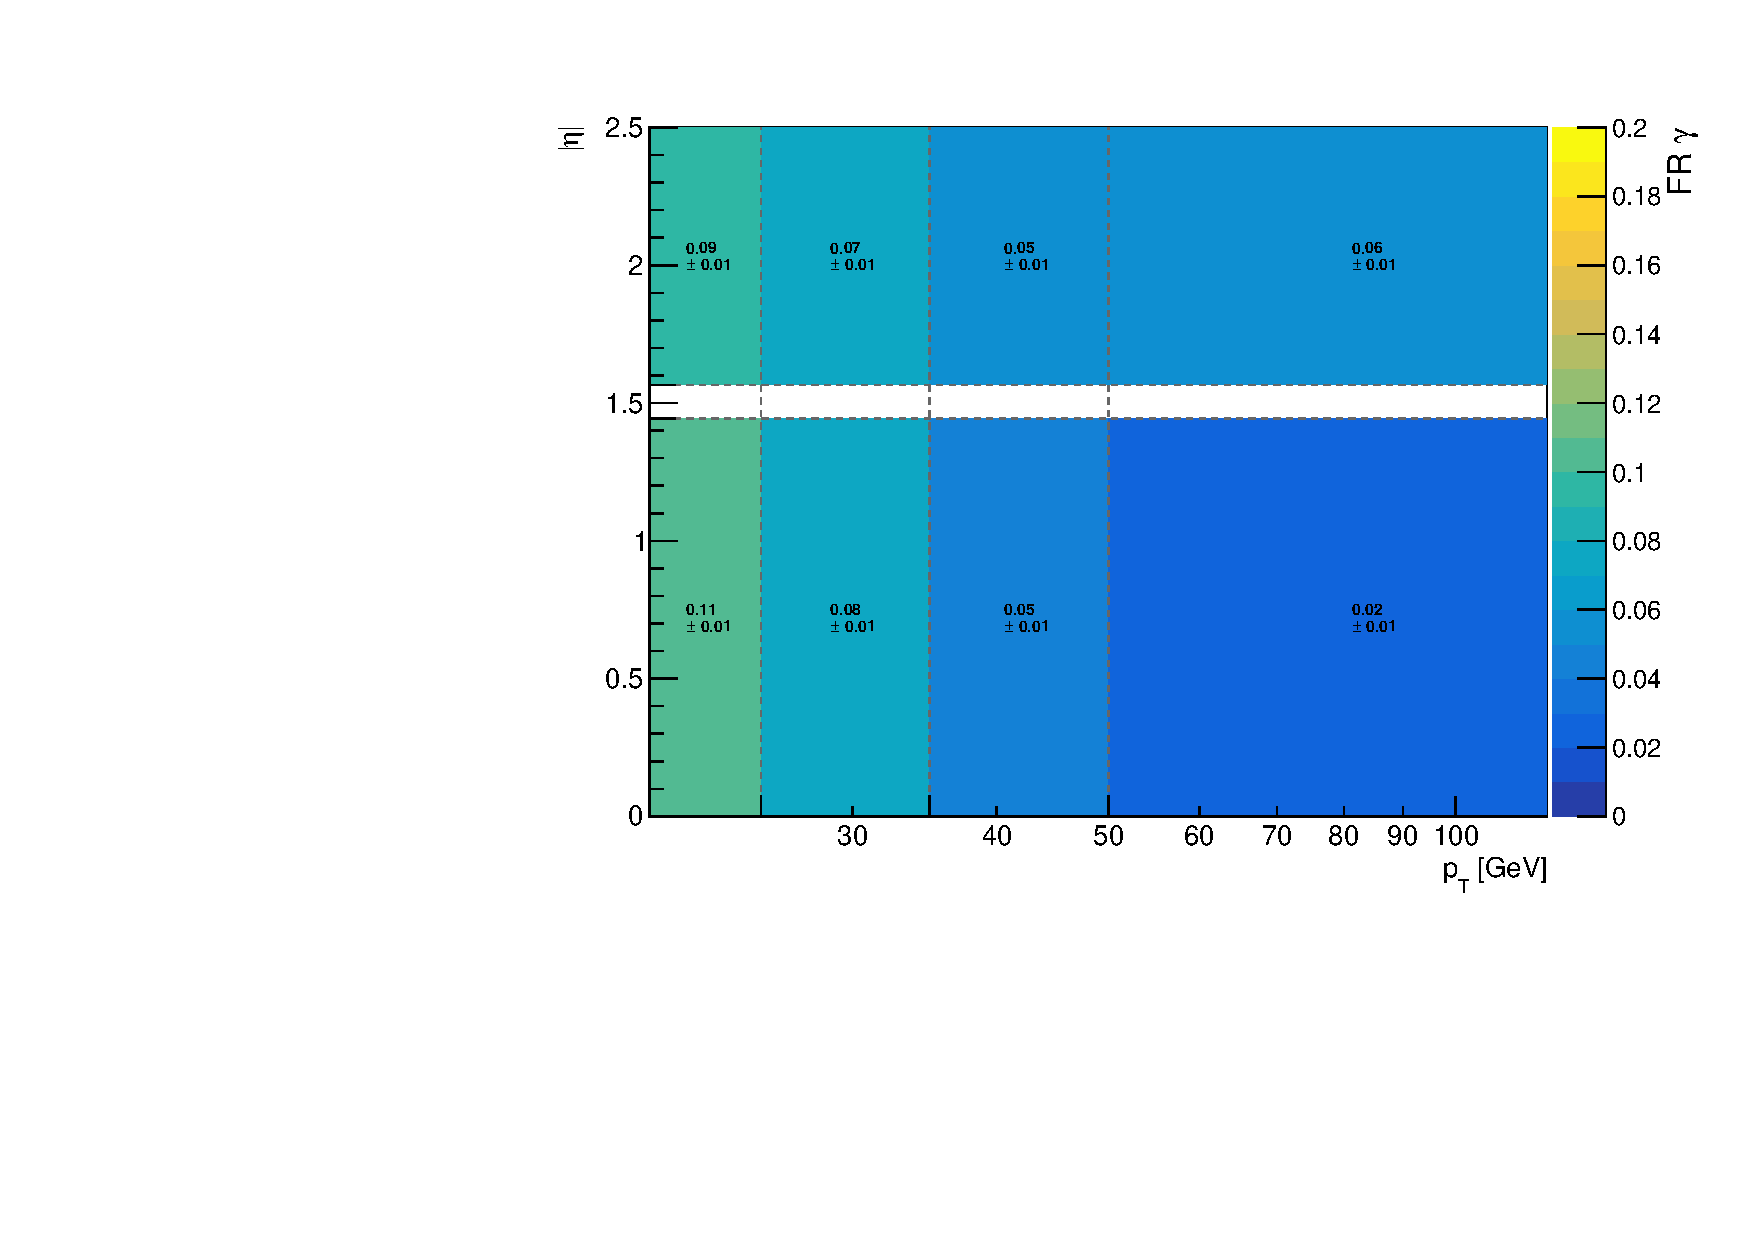
\includegraphics[width=.5\textwidth]{Figures/PhFR/FR_VLtoL_pt-aeta_2m+x_data-ZGToLLG_2018.pdf}}
\caption{Photon non-prompt rate as measured in 2018 data (with prompt $Z\gamma$ subtraction) in events with different lepton flavours for the Z boson.}
\label{fig:phFR_2e2m}
\end{figure}

The test is repeated for different flavours of the third lepton $\Pl^+ \Pl^- \Pepm$ and $\Pl^+ \Pl^- \PGmpm$, and is shown in Figure \ref{fig:phFR_em}.

\begin{figure}
\subfigure [$\ell^+ \ell^- e^\pm$]   {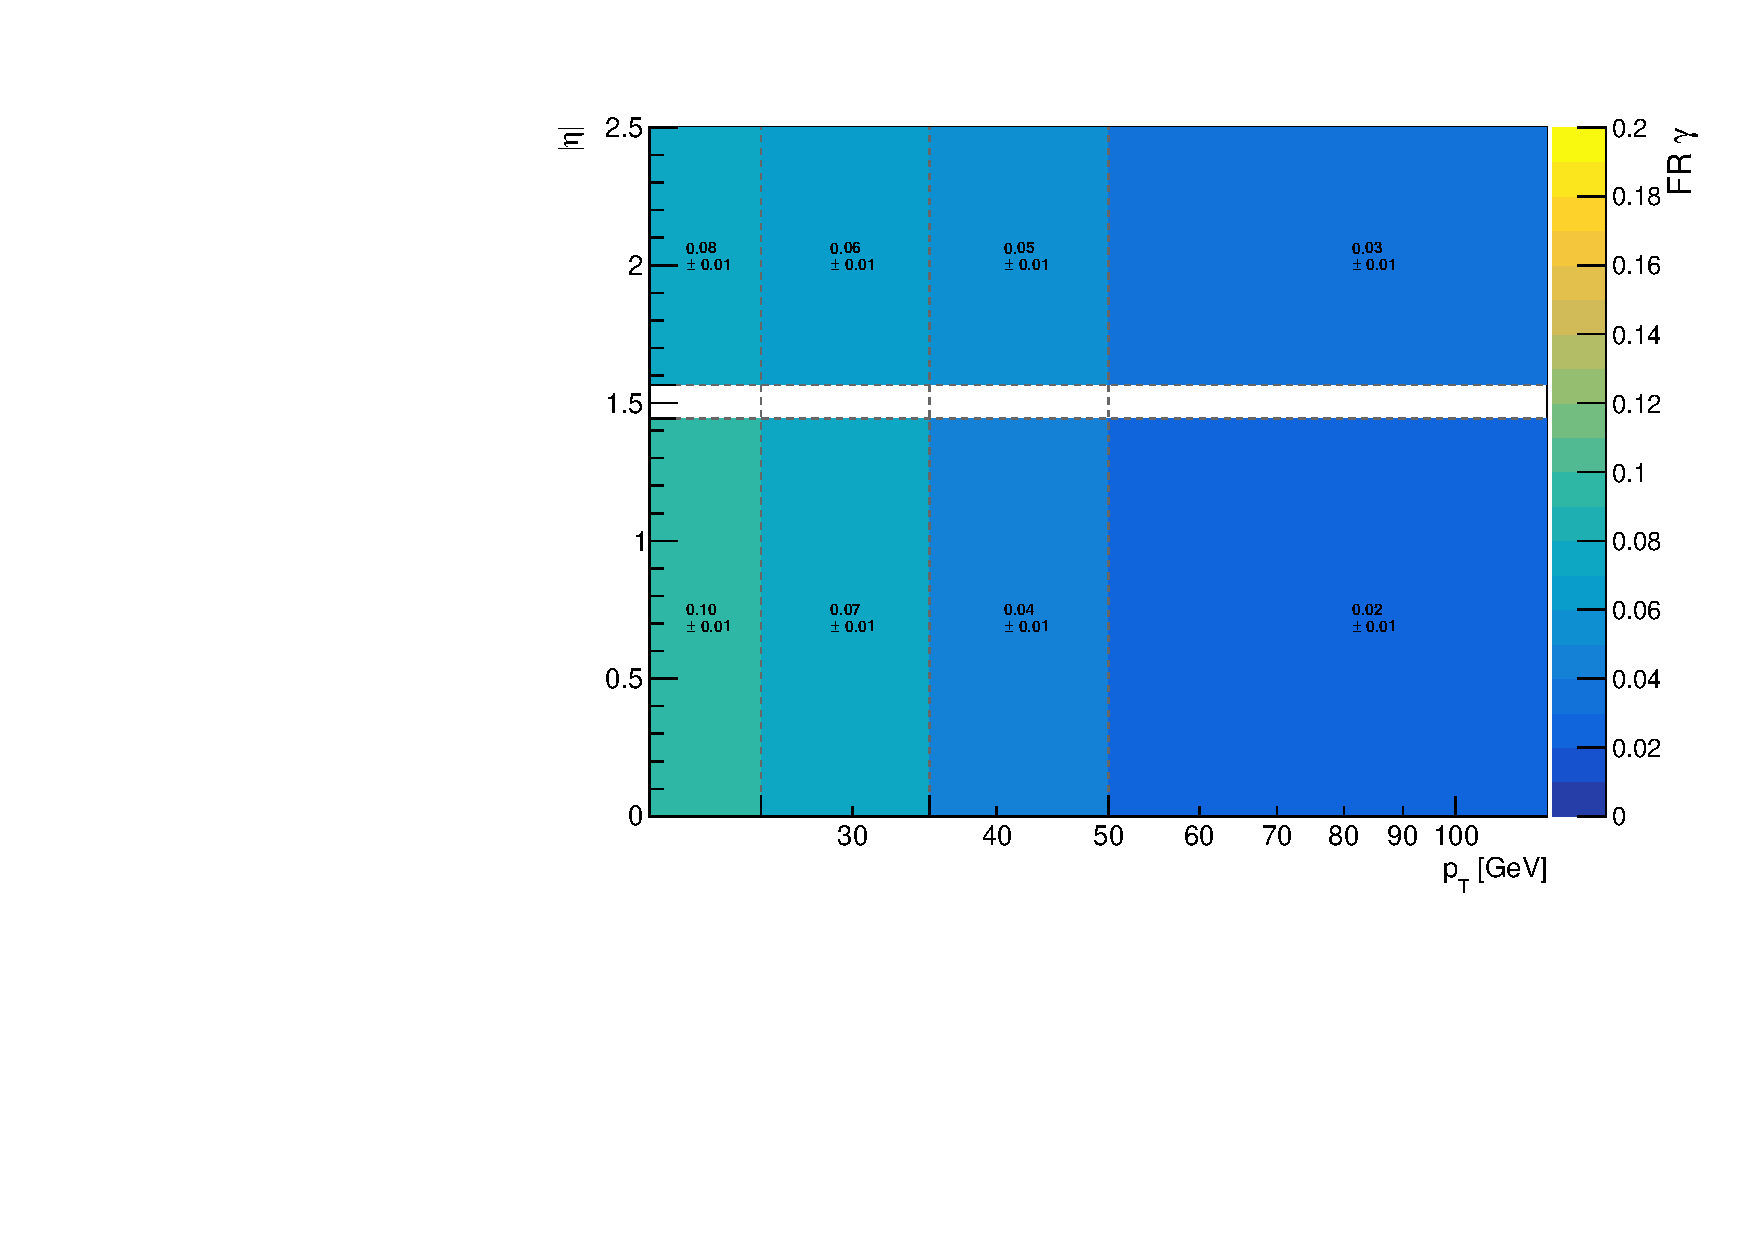
\includegraphics[width=.5\textwidth]{Figures/PhFR/FR_VLtoL_pt-aeta_2x+e_data-ZGToLLG_2018.pdf}}%
\subfigure [$\ell^+ \ell^- \mu^\pm$] {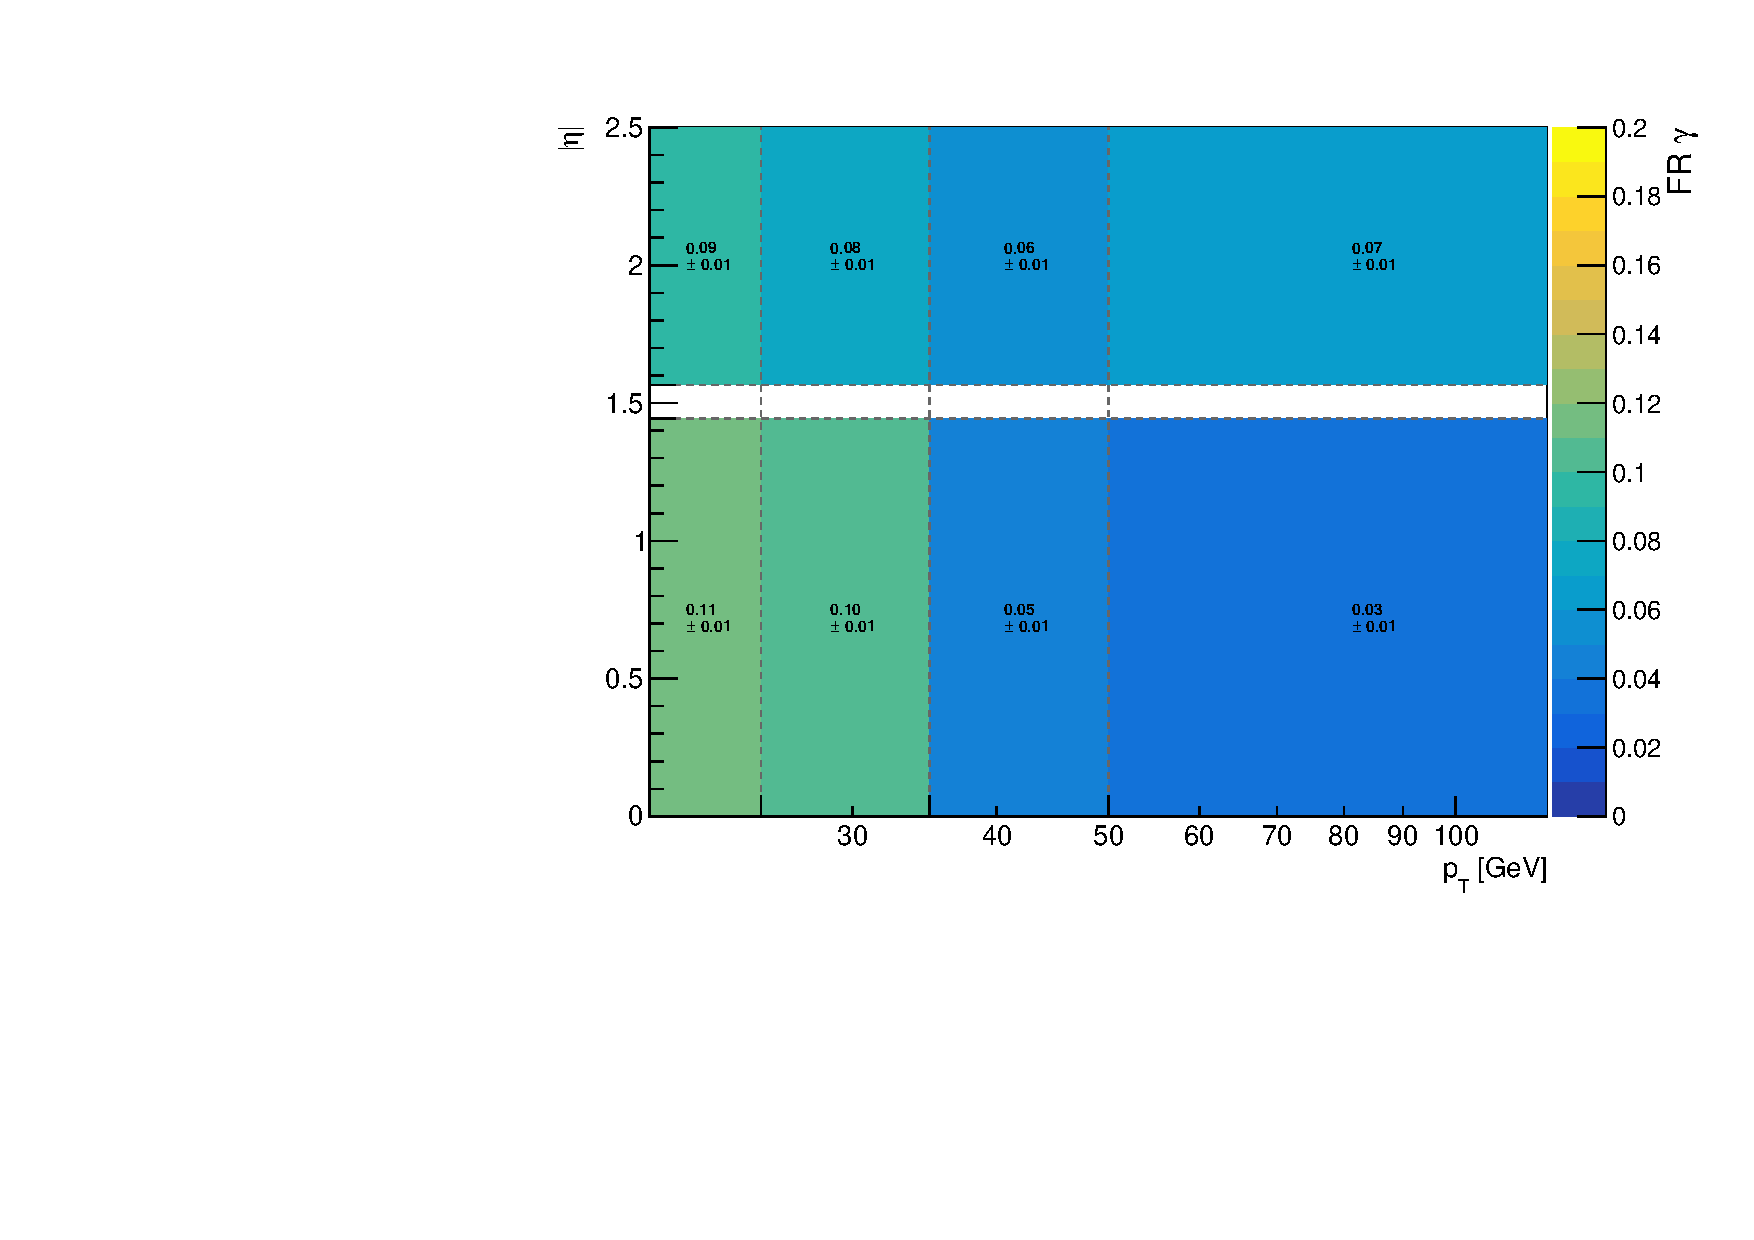
\includegraphics[width=.5\textwidth]{Figures/PhFR/FR_VLtoL_pt-aeta_2x+m_data-ZGToLLG_2018.pdf}}
\caption{Photon non-prompt rate as measured in 2018 data (with prompt $Z\gamma$ subtraction) in events with different flavours for the third lepton.}
\label{fig:phFR_em}
\end{figure}

Another test is performed by separating event where the third lepton passes/fails the tight analysis selection, shown in Figure \ref{fig:phFR_PF}.
In this case the two fake rates are not perfectly compatible.
However the number of events where the lepton passes the tight selection is
much smaller than the alternative, resulting in larger statistical uncertainties.

\begin{figure}
\subfigure [$\ell^+ \ell^- \ell^\pm_{PASS}$] {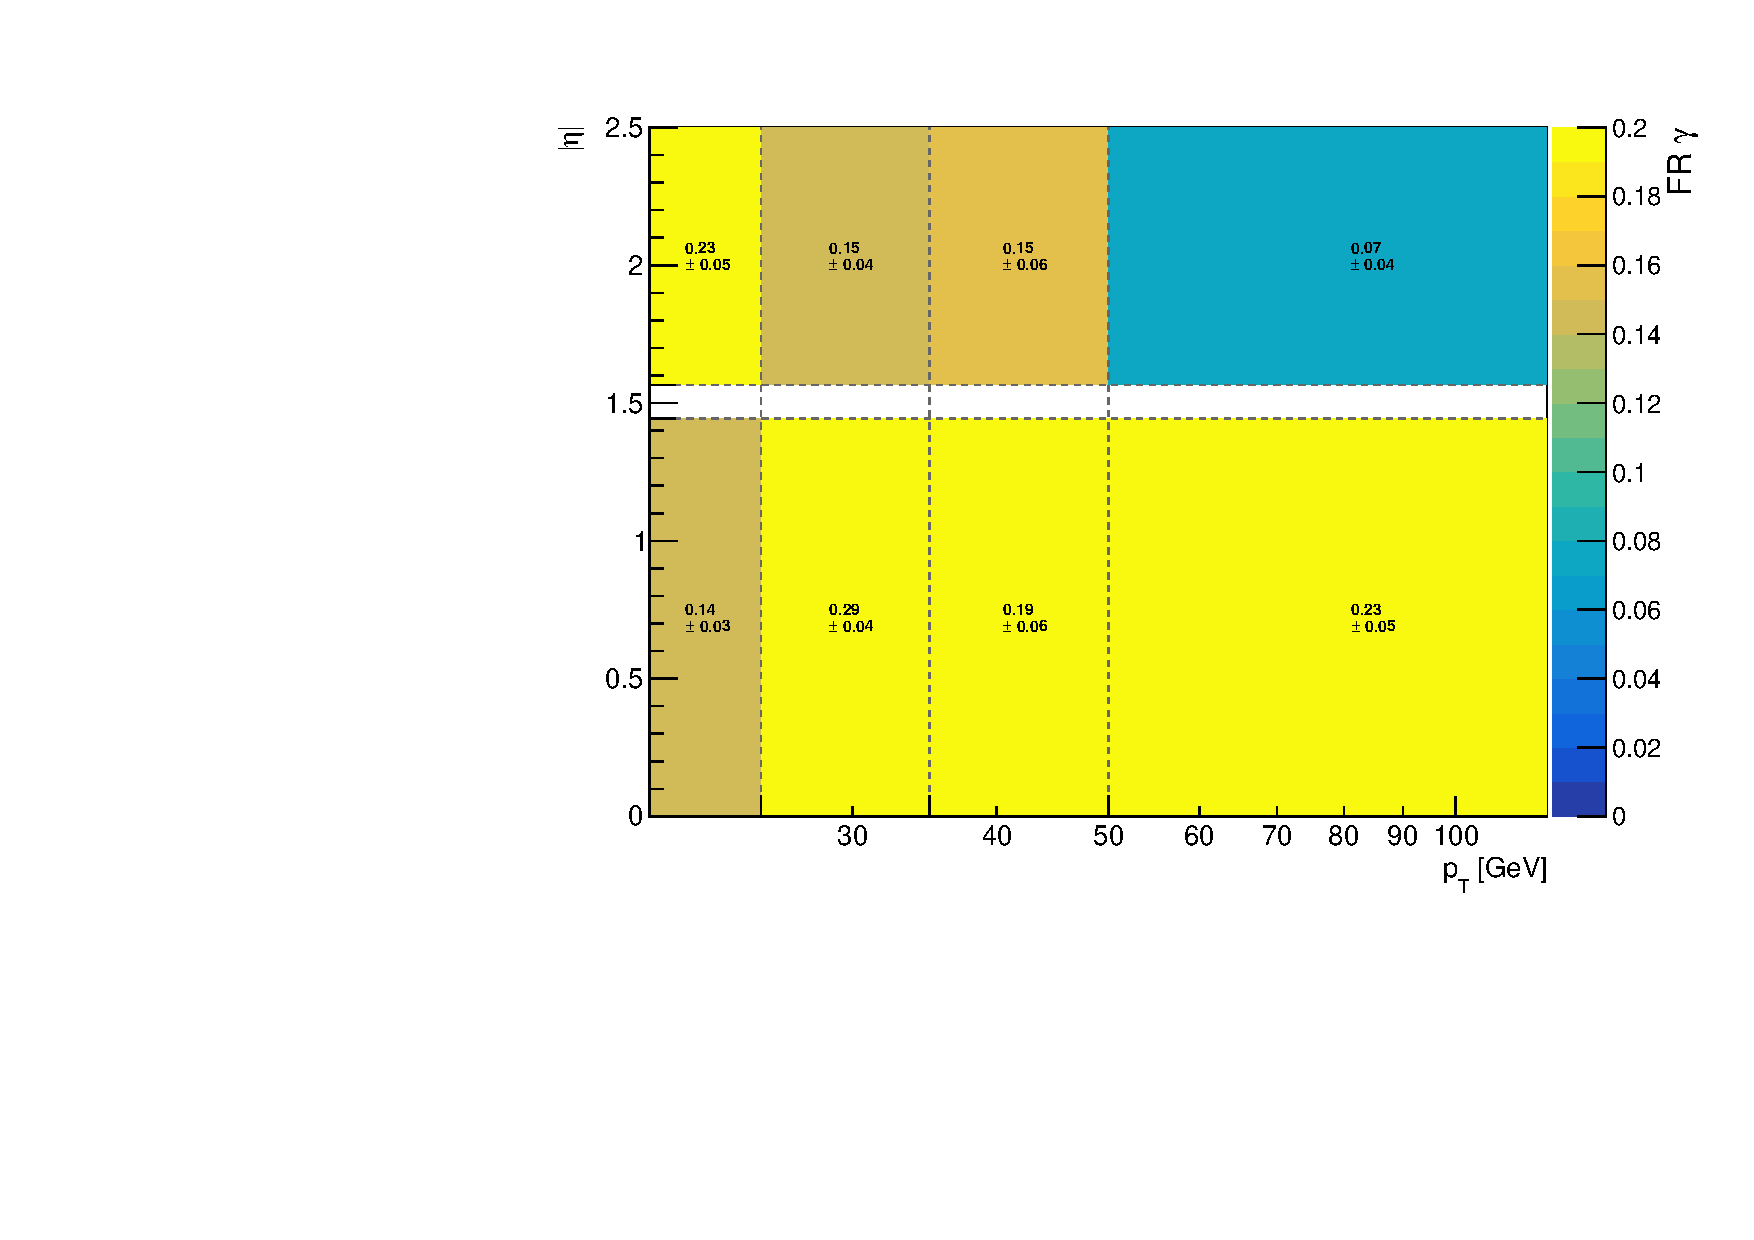
\includegraphics[width=.5\textwidth]{Figures/PhFR/FR_VLtoL_pt-aeta_2x+P_data-ZGToLLG_2018.pdf}}%
\subfigure [$\ell^+ \ell^- \ell^\pm_{FAIL}$] {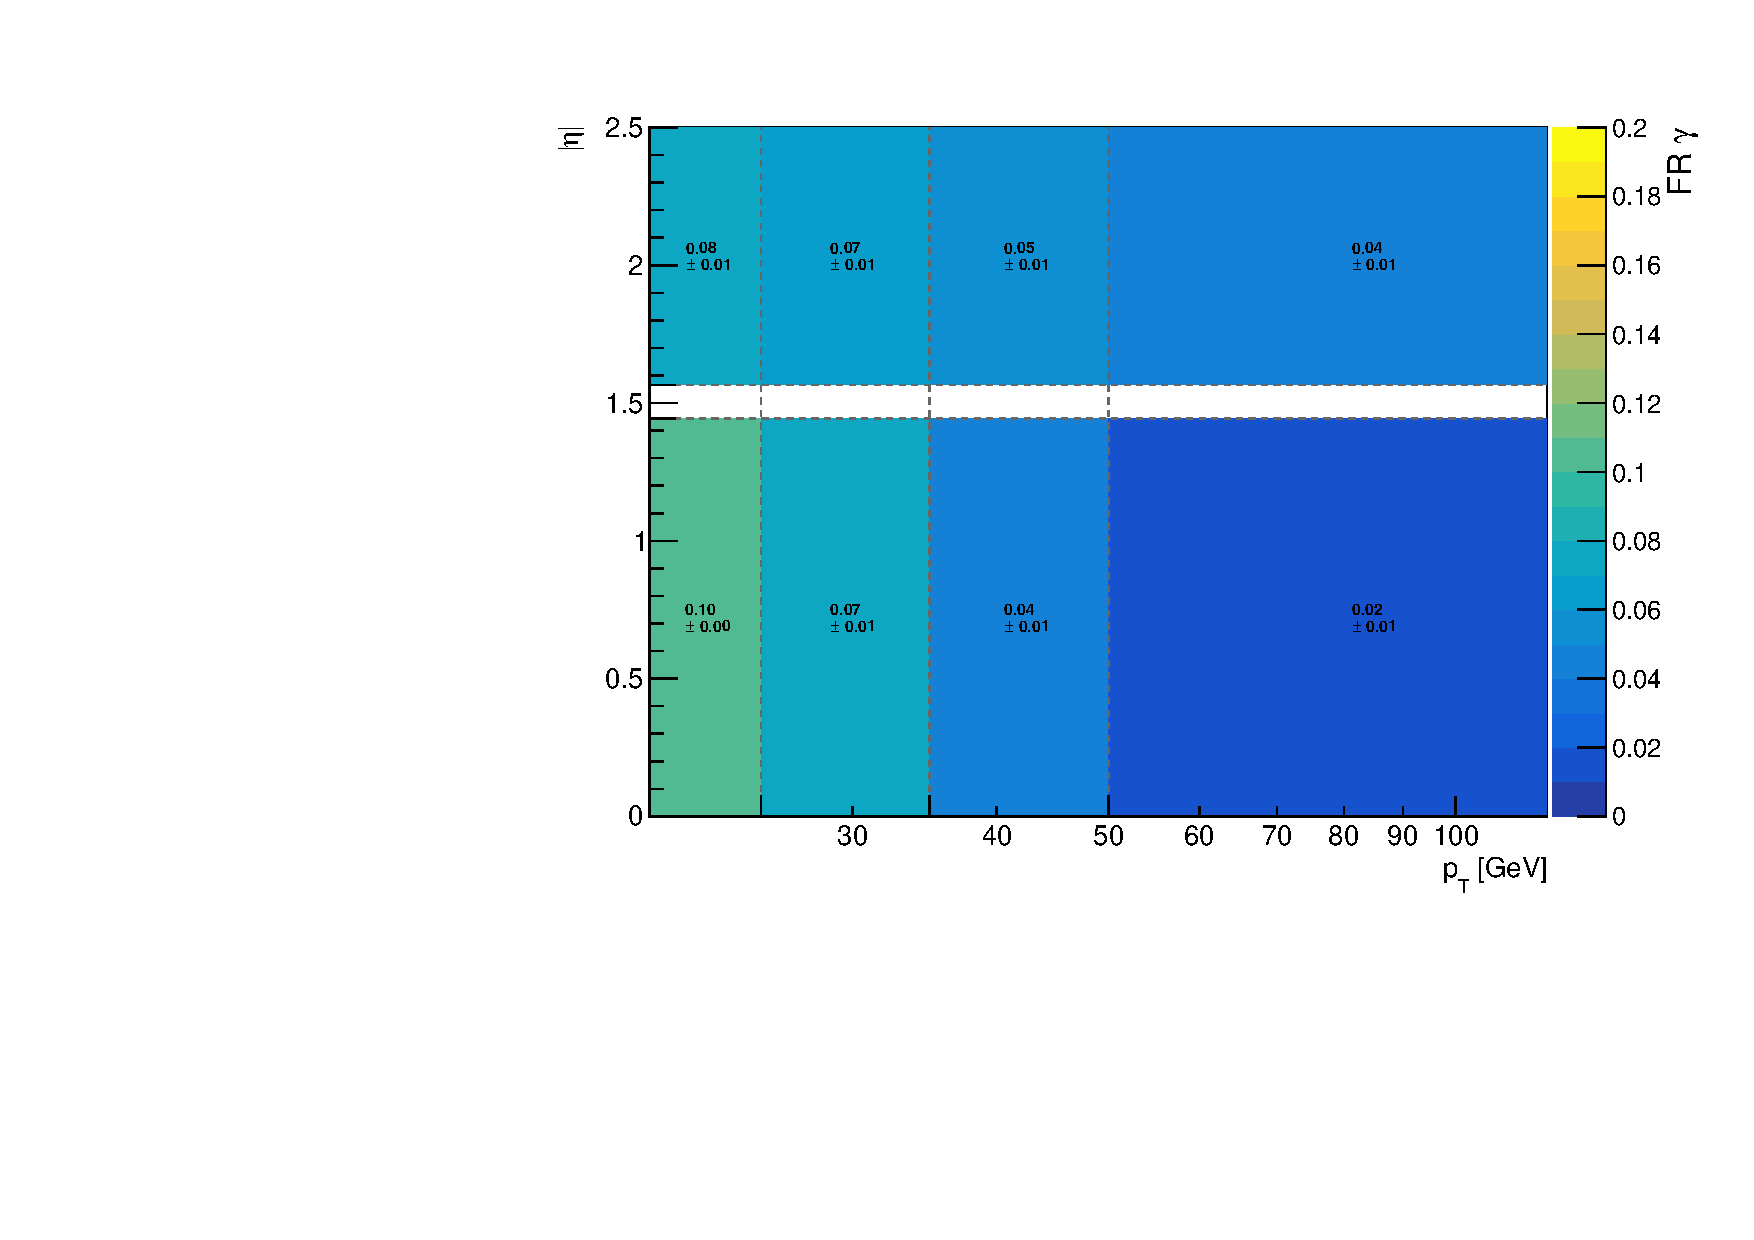
\includegraphics[width=.5\textwidth]{Figures/PhFR/FR_VLtoL_pt-aeta_2x+F_data-ZGToLLG_2018.pdf}}
\caption{Photon non-prompt rate as measured in 2018 data (with prompt $Z\gamma$ subtraction) in events where the third lepton passes/fails the tight selection, regardless of its flavour.}
\label{fig:phFR_PF}
\end{figure}

The trend for each $(p_{T}, |\eta|)$ bin for the different data-taking periods can be seen in Figure \ref{fig:phFR_time}.
It appears that, within the uncertainties, the measurements for each bin are compatible across the years,
and that a single rate for the whole \Run2 could be derived.
However, the results presented in this analysis use separate fake rates for each data-taking year
to minimize the correlation among the different periods.

\begin{figure}
\centering
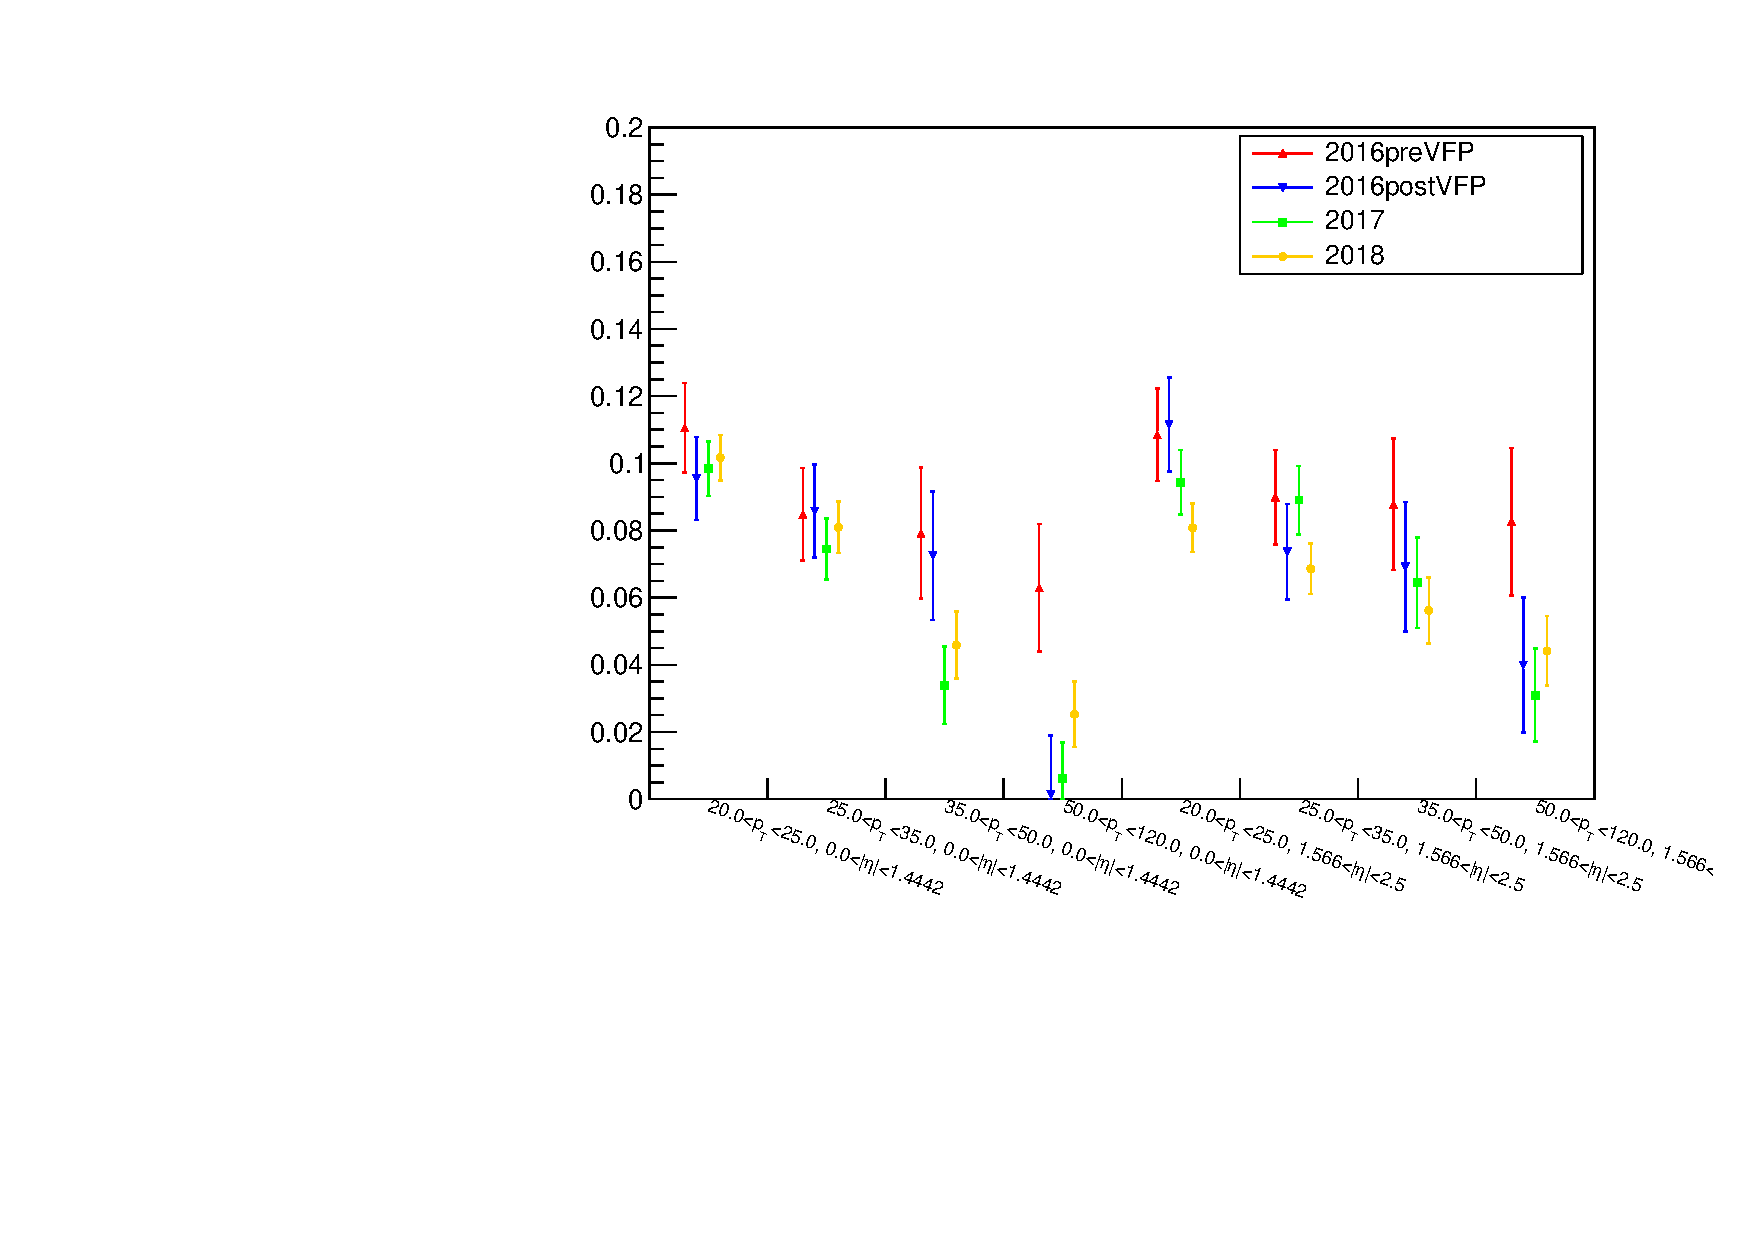
\includegraphics[height=.33\textheight]{Figures/PhFR/FR_VLtoL_pt-aeta_data-ZGToLLG_binEvol.pdf}
\caption{Photon non-prompt rate in different data-taking periods, for different bins of pseudorapidity and momentum.
  The year 2016 is split into ``preVFP'' and ``postVFP'' to model an issue in the readout chip in the tracker, explained in detail Section~\ref{sec:APV}.}
\label{fig:phFR_time}
\end{figure}

\subsubsection{Photon fake rate application}
The Fake Rate is then applied to events in the CR4P\_1F, CR3P\_1F and CR2P\_1F regions to estimate the non-prompt contribution in SR4P\_1P, SR3P\_1P, SR3P\_1P respectively.
The events with a fake photon can be reconstructed in the corresponding signal or application region
with a probability given by the fake rate.
The number of such events in the two regions is:
\begin{equation}
  \begin{split}
    \label{eq:fakeRate_explanation_part1}
    N^{bkg}_{4P\_1P} &= \sum f_i N^{bkg}
    \\
    N^{bkg}_{4P\_1F} &= \sum ( 1-f_i ) N^{bkg}
  \end{split}
\end{equation}
where $N^{bkg}$ is the total number of events that have a fake photon, regardless of the region they are classified into.
From this it follows that the number of background events in the signal region is:
\begin{equation}
  \label{eq:fakeRate_explanation_part2}
  N^{bkg}_{4P\_1P} = \sum \frac{f_i}{1-f_i} N_{4P\_1F}
\end{equation}

The transfer factor
$\text{TF}^\gamma(\pt, \eta) = \frac{f^\gamma}{1-f^\gamma}$,
where $f^\gamma$ is the Fake Rate estimated in the measurement region,
is used to reweight the events in the application region and obtain
the estimate of the fake photon background.

\paragraph{Usage of the MVA based ID\\}
Kinematic photons that pass the MVA-based working points \texttt{wp90} and \texttt{wp80} are also considered,
given the improved performance of the MVA ID over the cut-based one.
The drawback of these working points is the reduced size of the application region containing
photons that pass the looser selection (\texttt{wp90}) and fail the more strict one (\texttt{wp80}),
as shown in Figure~\ref{fig:SR4P_lead_90not80},
compared to the equivalent for the cut-based ID working point
in which photons are required to pass the VeryLoose ID and fail the Loose ID.

Unlike a cut-based selection, it is not possible to invert only part of the MVA based ID.
The only way to derive a looser working point is to redo the optimization of the raw MVA score,
and then study the efficiency of such selection in data and simulation to derive scale factors.
Both of these studies are outside the scope of this analysis.
Therefore it is not possible to estimate the fake photon background in the four lepton channel
with a Tight-To-Loose method using the two working points \texttt{wp90} and \texttt{wp80} of the MVA based ID.

Another possibility is to measure a fake rate between the kinematic selection and the looser MVA working point, \texttt{wp90}.
However, the former is too loose and the selected fakes have signatures that are very different from those of prompt photons.
This would make the assumption that the transfer factor is the same in the measurement and application regions quite unstable.

\begin{figure}
  \centering
  \subfigure [$\pt   $ of $\PGg^{\tt{wp90} \land !\tt{wp80}}$] {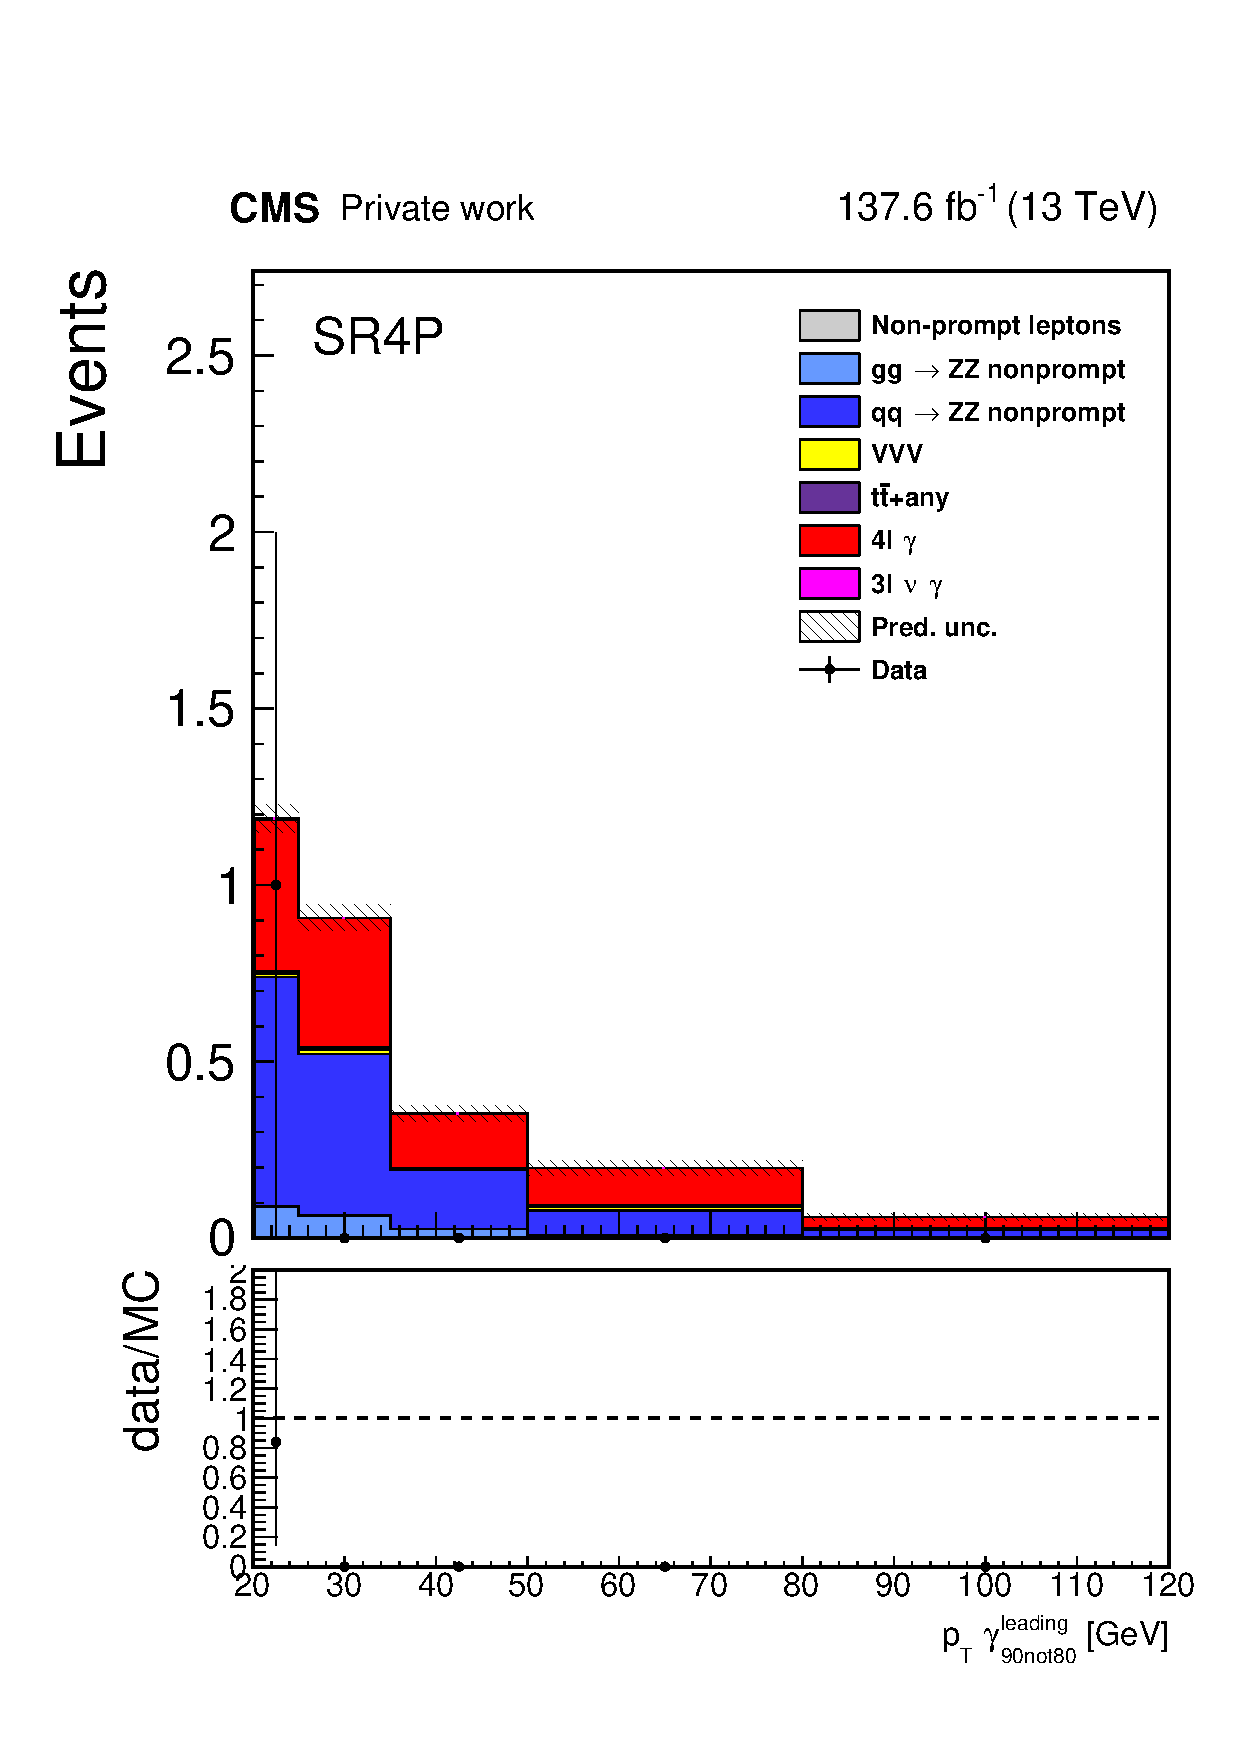
\includegraphics[width=.333333333\textwidth]{VVGammaAnalyzer/Run2/lepCR/SR4P/lead_90not80_pt_pow.pdf}}%
  \subfigure [$|\eta|$ of $\PGg^{\tt{wp90} \land !\tt{wp80}}$] {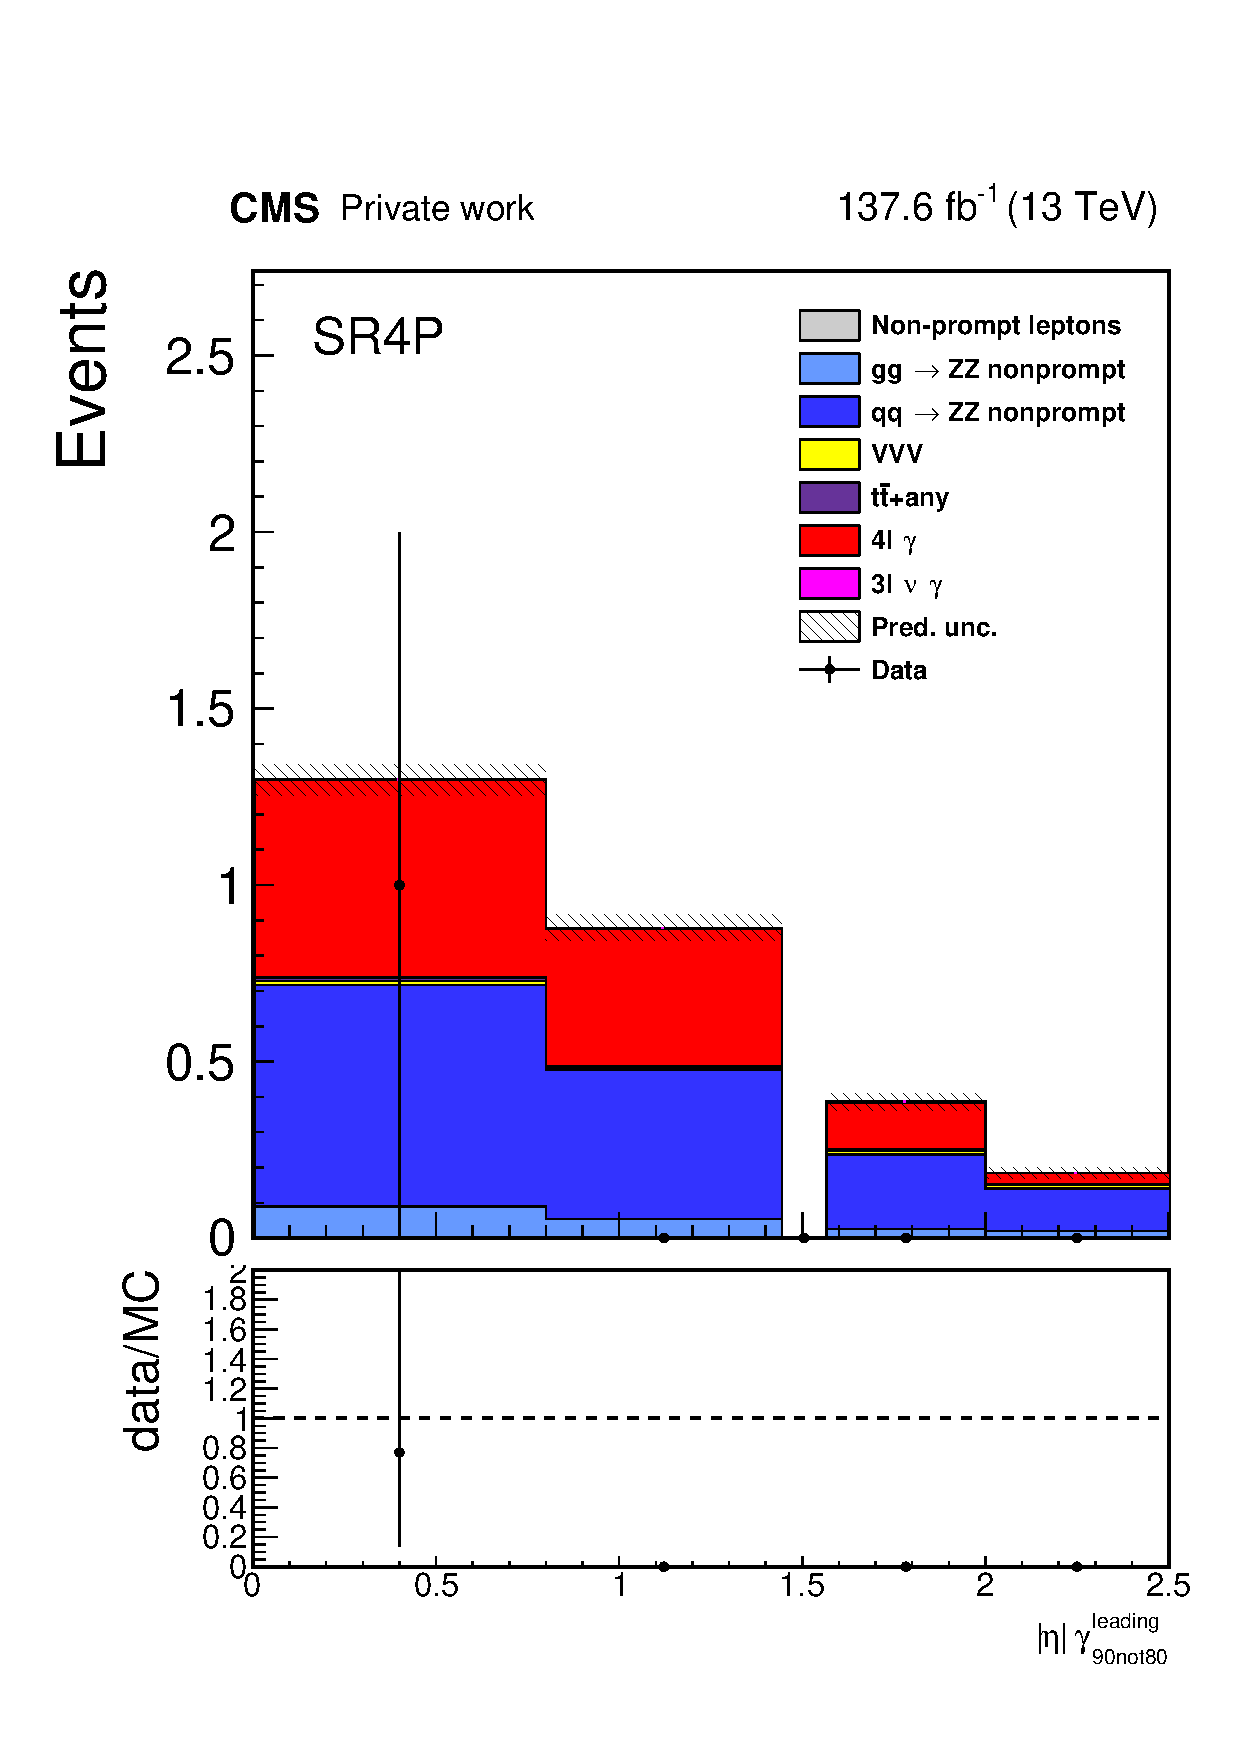
\includegraphics[width=.333333333\textwidth]{VVGammaAnalyzer/Run2/lepCR/SR4P/lead_90not80_aeta_pow.pdf}}%
  \subfigure [$\sieie$ of $\PGg^{\tt{wp90} \land !\tt{wp80}}$] {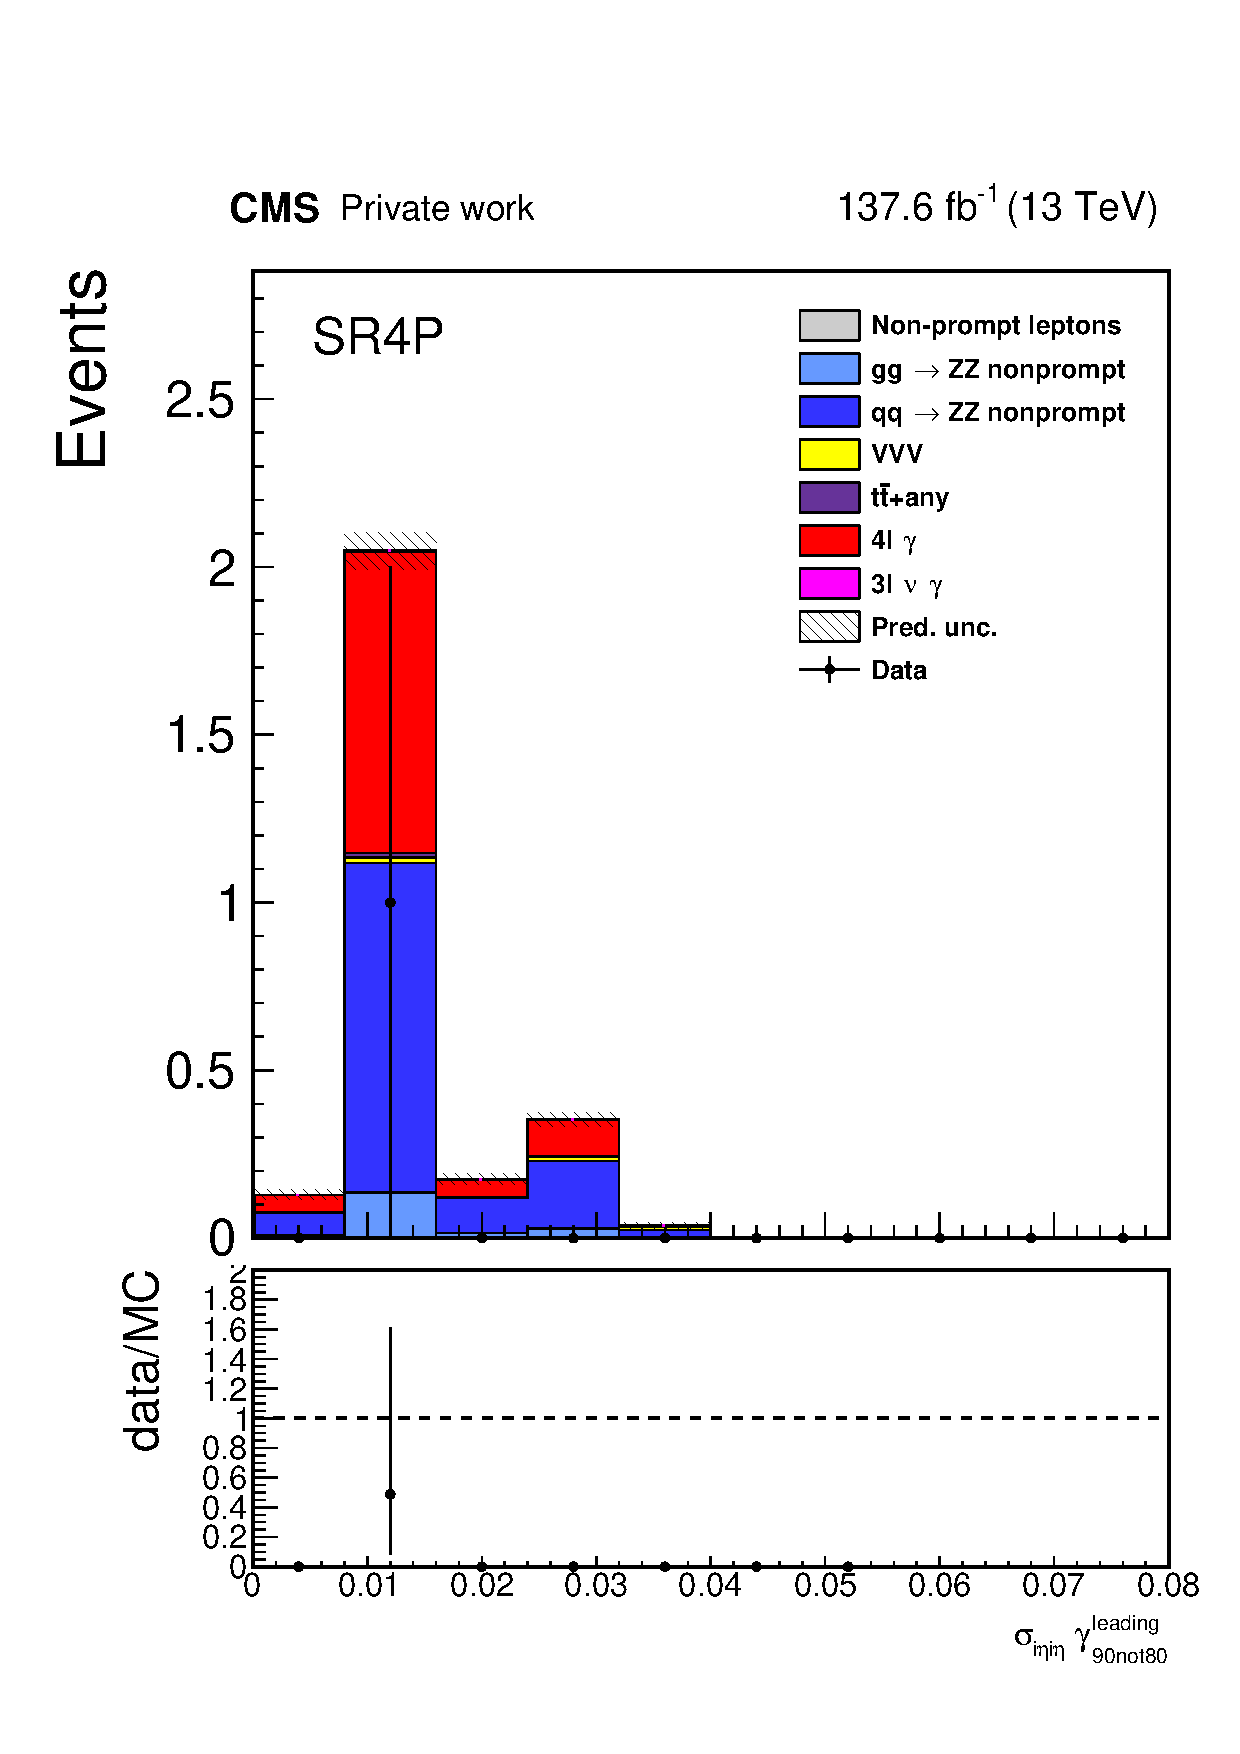
\includegraphics[width=.333333333\textwidth]{VVGammaAnalyzer/Run2/lepCR/SR4P/lead_90not80_sieie_pow.pdf}}
  \caption{Transverse momentum, pseudorapidity and \sieie of photons
    passing the \texttt{wp90} and failing the \texttt{wp80} working point of the MVA based ID
    in the region with four leptons passing the tight selection.
    This would be the photon fake rate application region
    for a tight-to-loose method using the two MVA working points.
    }
  \label{fig:SR4P_lead_90not80}
\end{figure}

Therefore, the results obtained using the MVA ID are derived without the data-driven estimate of fake photons.
In this case, the MC prediction of backgrounds which contain \nonprompt or misidentified photons is used.


\section{Dataset and samples}
\label{sec:datasets}

\subsection{Trigger selection}
\label{sec:triggers}
Several HLT paths are used to select events which present a certain number of electrons or muons in the final state.
Due to the evolution of trigger requirements with instantaneous LHC luminosity,
the collection of HLT paths used in this analysis is different for each data taking year.

The HLT paths used for collision data are listed in Tables~\ref{tab:triggerpaths2016}, \ref{tab:triggerpaths2017} and \ref{tab:triggerpaths2018},
together with
%% their L1 seed, prescale value and
the associated primary dataset.
The trigger paths and the disambiguation scheme are the same used in Reference~\cite{CMS-PAS-HIG-19-001},
and they were optimised for the phase space of the $\PH \to \PZ \PZst \to 4\Pl$ analysis.

\begin{table*}
  \caption{Trigger paths used in 2016 collision data. All triggers have prescale = 1.}
  \label{tab:triggerpaths2016}
  \centering
  \small
  \begin{tabular}{ l l l }
    \toprule %--------------------------------------------------------------------------------------------------------------------------
    Trigger description & Requirements & Primary Dataset \\
    \midrule %--------------------------------------------------------------------------------------------------------------------------
    Double isolated electron     & $\pt^{\Pe_1}, \pt^{\Pe_2} > 17, 12 \GeVc$                 & \multirow{4}{*}{DoubleEG} \\
    Double isolated electron     & $\pt^{\Pe_1}, \pt^{\Pe_2} > 23, 12 \GeVc$                 & \\
    Double isolated GSF electron & $\pt^{\Pe_1}, \pt^{\Pe_2} > 33, 33 \GeVc$                 & \\
    Triple isolated electron     & $\pt^{\Pe_1}, \pt^{\Pe_2}, \pt^{\Pe_3} > 16, 12, 8 \GeVc$ & \\
    \hline
    Double isolated muon & $\pt^{\PGm_1}, \pt^{\PGm_2} > 17, 8 \GeVc$                   & \multirow{3}{*}{DoubleMuon} \\
    Double isolated muon\hyperlink{tab:triggerpaths2016:fn1}{${}^1$}
                         & $\pt^{\PGm_1}, \pt^{\PGm_2} > 17, 8 \GeVc$                   & \\
    Triple isolated muon & $\pt^{\PGm_1}, \pt^{\PGm_2}, \pt^{\PGm_3} > 12, 10, 5 \GeVc$ & \\
    \hline
    Tracker muon \!+\! isolated electron & $\pt^{\PGm}, \pt^{\Pe} > 8 , 17$                   & \multirow{7}{*}{MuonEG} \\
    Tracker muon \!+\! isolated electron & $\pt^{\PGm}, \pt^{\Pe} > 8 , 23$                   & \\
    Tracker muon \!+\! isolated electron & $\pt^{\PGm}, \pt^{\Pe} > 17, 12$                   & \\
    Tracker muon \!+\! isolated electron & $\pt^{\PGm}, \pt^{\Pe} > 23, 12$                   & \\
    Tracker muon \!+\! isolated electron & $\pt^{\PGm}, \pt^{\Pe} > 23, 8 $                   & \\
    Tracker muon \!+\! double electron   & $\pt^{\PGm},\pt^{\Pe_1},\pt^{\Pe_2} >8,12,12\GeVc$ & \\
    Double tracker muon + electron   & $\pt^{\PGm_1},\pt^{\PGm_2},\pt^{\Pe}>9,9,9\GeVc$   & \\
    \hline
    Single tight ID central electron & $\pt^{\Pe}>25$, $|\eta^\Pe| < 2.1$ & \multirow{3}{*}{SingleElectron} \\
    Single tight ID electron         & $\pt^{\Pe}>27$                     & \\
    Single tight ID GSF electron     & $\pt^{\Pe}>27$, $|\eta^\Pe| < 2.1$ & \\
    \hline
    Single isolated muon & $\pt^{\PGm}>20$ & \multirow{2}{*}{SingleMuon} \\
    Single isolated muon & $\pt^{\PGm}>22$ & \\
    \bottomrule %-----------------------------------------------------------------------------------------------------------------------
    \noalign{\vspace{.5ex}} % small vertical space
    \multicolumn{3}{l}{\quad\hypertarget{tab:triggerpaths2016:fn1}{1}: $\mu_1$ is global, $\mu_2$ is tracker muon} \\
  \end{tabular}
\end{table*}

\begin{table*}
  \caption{Trigger paths used in 2017 collision data. All triggers have prescale = 1.}
  \label{tab:triggerpaths2017}
  \centering
  \small
  \begin{tabular}{ l l l }
    \toprule %--------------------------------------------------------------------------------------------------------------------------
    Trigger description & Requirements & Primary Dataset \\
    \midrule %--------------------------------------------------------------------------------------------------------------------------
    Double isolated electron & $\pt^{\Pe_1}, \pt^{\Pe_2} > 23, 12 \GeVc$                 & \multirow{3}{*}{DoubleEG} \\
    Double GSF electron      & $\pt^{\Pe_1}, \pt^{\Pe_2} > 33, 33 \GeVc$                 & \\
    Triple electron          & $\pt^{\Pe_1}, \pt^{\Pe_2}, \pt^{\Pe_3} > 16, 12, 8 \GeVc$ & \\
    \hline
    Double isolated muon & $\pt^{\PGm_1}, \pt^{\PGm_2} > 17, 8 \GeVc,\ m_{\PGm\PGm} > 3.8\GeVcc$ & \multirow{4}{*}{DoubleMuon} \\
    Double isolated muon & $\pt^{\PGm_1}, \pt^{\PGm_2} > 17, 8 \GeVc,\ m_{\PGm\PGm} > 8  \GeVcc$ & \\
    Triple muon          & $\pt^{\PGm_1}, \pt^{\PGm_2}, \pt^{\PGm_3} > 12, 10, 5\GeV$            & \\
    Triple muon          & $\pt^{\PGm_1}, \pt^{\PGm_2}, \pt^{\PGm_3} > 10,  5, 5\GeV$            & \\
    \hline
    Iso muon \!+\! iso electron & $\pt^\PGm, \pt^\Pe > 23, 12 \GeVc$                            & \multirow{7}{*}{MuonEG} \\
    Iso muon \!+\! iso electron & $\pt^\PGm, \pt^\Pe > 8 , 23 \GeVc$                            & \\
    Iso muon \!+\! iso electron & $\pt^\PGm, \pt^\Pe > 12, 23 \GeVc$                            & \\
    Iso muon \!+\! iso electron & $\pt^\PGm, \pt^\Pe > 23, 12 \GeVc$                            & \\
    Double muon \!+\! electron            & $\pt^{\PGm_1}, \pt^{\PGm_2}, \pt^\Pe > 9,9,9 \GeVc$ & \\
    Muon \!+\! double electron            & $\pt^\PGm, \pt^{\Pe_1}, \pt^{\Pe_2} > 8,12,12\GeVc$ & \\
    Muon \!+\! double electron            & $\pt^\PGm, \pt^{\Pe_1}, \pt^{\Pe_2} > 8,12,12\GeVc$ & \\
    \hline
    Single tight ID electron & $\pt^\Pe > 35 \GeVc$ & \multirow{3}{*}{SingleElectron} \\
    Single tight ID electron & $\pt^\Pe > 38 \GeVc$ & \\
    Single tight ID electron & $\pt^\Pe > 40 \GeVc$ & \\
    \hline
    Single isolated muon & $\pt^\PGm > 27 \GeVc$ & SingleMuon \\
    \bottomrule %-----------------------------------------------------------------------------------------------------------------------
  \end{tabular}
\end{table*}

\begin{table*}
  \caption{Trigger paths used in 2018 collision data. All triggers have prescale = 1.}
  \label{tab:triggerpaths2018}
  \small
  \centering
  \begin{tabular}{ l l l }
    \toprule %--------------------------------------------------------------------------------------------------------------------------
    Trigger description & Requirements & Primary Dataset \\
    \midrule %--------------------------------------------------------------------------------------------------------------------------
    Double isolated electron    & $\pt^{\Pe_1}, \pt^{\Pe_2} > 23, 12 \GeVc$ & \multirow{3}{*}{EGamma} \\
    Double electron             & $\pt^{\Pe_1}, \pt^{\Pe_2} > 25, 25 \GeVc$ & \\
    Single isolated electron    & $\pt^\Pe > 32 \GeVc$                      & \\
    \hline
    Double isolated muon        & $\pt^{\PGm_1}, \pt^{\PGm_2} > 17, 8 \GeVc,\ m_{\PGm\PGm} > 3.8\GeVcc$ & DoubleMuon \\
    \hline
    Iso muon \!+\! iso electron & $\pt^\PGm, \pt^\Pe > 23, 12 \GeVc$                  & \multirow{5}{*}{MuonEG} \\
    Iso muon \!+\! iso electron & $\pt^\PGm, \pt^\Pe >  8, 23 \GeVc$                  & \\
    Iso muon \!+\! iso electron & $\pt^\PGm, \pt^\Pe > 12, 23 \GeVc$                  & \\
    Iso muon \!+\! iso electron & $\pt^\PGm, \pt^\Pe > 23, 12 \GeVc$                  & \\
    Double muon \!+\! electron  & $\pt^{\PGm_1}, \pt^{\PGm_2}, \pt^\Pe > 9,9,9 \GeVc$ & \\
    \hline
    Single isolated muon        & $\pt^\PGm > 24 \GeVc$ & SingleMuon \\
    \bottomrule %-----------------------------------------------------------------------------------------------------------------------
  \end{tabular}
\end{table*}

They are grouped according to the kind of event selected.
Each trigger path requires the presence of one or more particles above a certain transverse momentum threshold.
Each trigger path in these groups additionally requires the event to satisfy conditions regarding particle identification from the sub-detector systems,
or isolation from other objects in a cone around the triggering particle.
The \textit{Double Electron} triggers select events containing in the final state at least two electrons.
Similarly, \textit{Triple Electron} triggers target events containing three electrons.
\textit{Double Muon} and \textit{Triple Muon} triggers target events with at least two and three muons, respectively,
while \textit{Muon Electron} triggers select events containing in the final state at least one muon and one electron.
\textit{Single Muon} triggers select events with at least one muon,
while \textit{Single Electron} triggers select events containing in the final state at least one electron.


\subsection{CMS data}
This analysis uses a data sample recorded by the CMS experiment at a centre-of-mass energy of 13\TeV during 2016, 2017 and 2018 corresponding to $\Lumi = 137 \fbinv$ of data.
Only data that passed the quality certification by all detector subsystems is used in the analysis.
%% and only luminosity sections included in the respective golden JSONs are used for further analysis.
The luminosity measurements are carried out by experts within the collaboration according to the methodology described in Ref. \cite{CMS:LUM-17-003}, for each year of data-taking \cite{CMS:LUM-17-004, CMS:LUM-18-002}.

The samples used correspond to the so called ``UltraLegacy reprocessing'', which contains the most recent calibrations of all the physics objects reconstruction and identification criteria, as well as scale factors and uncertainties.
The simulations for 2016 are split into ``preVFP'' and ``postVFP'' to model the effect
of an inefficiency in a readout chip in the tracker, explained in Section~\ref{sec:APV}, which was resolved during data taking.
%% The MINIAOD format is chosen to perform the analysis.

The analysis relies on five different Primary Datasets (PD),
{\it DoubleEG}, {\it DoubleMu}, {\it MuonEG}, {\it SingleElectron}, and {\it SingleMuon},
each of which combines a certain collections of HLT paths, whose exact requirements depend on the year of data
taking. {\it DoubleEG} and {\it SingleElectron} are merged into {\it EGamma} in 2018.
To avoid duplicate events from different primary datasets, events are taken:

\begin{itemize}
\item from DoubleEG if they pass the diEle %(\texttt{HLT\_EleXX\_EleYY\_CaloIdXX\_TrackIdXX\_IsoXX(\_DZ)} )
  or triEle triggers, %(\texttt{HLT\_EleXX\_EleYY\_EleZZ\_CaloIdXX\_TrackIdXX}) where XX, YY and ZZ are year-dependent thresholds
\item from DoubleMuon if they pass the diMuon %(\texttt{HLT\_MuXX\_TrkIsoVVL\_MuYY\_TrkIsoVVL})
  or triMuon %(\texttt{HLT\_TripleMu\_XX\_YY\_ZZ})
  triggers and fail the diEle and triEle triggers,
\item from MuEG if they pass the MuEle %(\texttt{HLT\_MuXX\_TrkIsoXX\_EleYY\_CaloIdYY\_TrackIdYY\_IsoYY})
  or MuDiEle %(\texttt{HLT\_MuXX\_DiEleYY\_CaloIdYY\_TrackIdYY})
  or DiMuEle %(\texttt{HLT\_DiMuXX\_EleYY\_CaloIdYY\_TrackIdYY})
  triggers and fail the diEle, triEle, diMuon and triMuon triggers,
\item from SingleElectron if they pass the singleElectron trigger %(\texttt{HLT\_EleXX\_etaXX\_WPLoose/Tight(\_Gsf)})
  and fail all the above triggers.
\item from SingleMuon if they pass the singleMuon trigger %(\texttt{HLT\_IsoMuXX OR HLT\_IsoTkMuXX})
  and fail all the above triggers.
\end{itemize}

The used data sets are listed in Table~\ref{tab:datasamples}.%, along with the integrated luminosity.

\begin{table*}
  \caption{List of data samples used in the analysis. All runs for each of the 5 data streams are used, for a total of 76 primary datasets in the MINIAOD format.}
  \label{tab:datasamples}
  \centering
  \small
  \begin{tabular}{l l}
    \toprule
    \textbf{Data stream} &  \textbf{Run and reconstruction version}\\
    \midrule
    \begin{tabular}{@{}l}
      DoubleMuon\\
      DoubleEG\\
      MuonEG\\
      SingleMuon\\
      SingleElectron
    \end{tabular}&
    \begin{tabular}{@{}l}
      Run2016B-ver1\_HIPM\_UL2016\\
      Run2016B-ver2\_HIPM\_UL2016\\
      Run2016C-HIPM\_UL2016\\
      Run2016D-HIPM\_UL2016\\
      Run2016E-HIPM\_UL2016\\
      Run2016F-HIPM\_UL2016\\
      Run2016F-UL2016\\
      Run2016G-UL2016\\
      Run2016H-UL2016
    \end{tabular} \\
    \hline
    DoubleMuon     & Run2017B-UL2017\\
    DoubleEG       & Run2017C-UL2017\\
    MuonEG         & Run2017D-UL2017\\
    SingleMuon     & Run2017E-UL2017\\
    SingleElectron & Run2017F-UL2017\\
    \hline
    DoubleMuon & Run2018A-UL2018\\
    MuonEG     & Run2018B-UL2018\\
    SingleMuon & Run2018C-UL2018\\
    EGamma     & Run2018D-UL2018\\
    \bottomrule
  \end{tabular}
\end{table*}

\subsection{Simulation}
\label{sec:simulation}
\MGvATNLO 2.6.2 \cite{MGatNLO, Frederix_2018} is used to simulate the signal and most of the background contributions.
The simulation of $\PQq \PQq / \PQq \Pg \to \PZ \PZ \to 4 \Pl$ is done with \POWHEG~\cite{Nason:2004rx, Frixione:2007vw, Alioli:2010xd, Alioli:2008gx},
while $\Pg \Pg \to \PZ \PZ \to 4 \Pl$ is simulated with \MCFM~\cite{MCFM}.
The simulation of the hadronization and parton shower is done by coupling the matrix element generators with \PYTHIA~8~\cite{bierlich2022comprehensive, Sjostrand:2015} using the \textsc{CP5}~tune~\cite{CP5}.
The interaction of the particles with the CMS detector is simulated with \GEANTfour~\cite{GEANT}.
All samples are generated with the NNPDF 3.0 (in 2016) or 3.1 (2017-18) parton distribution functions (PDFs)~\cite{NNPDF2015}.
The MC samples are reweighed based on the per-event true number of interactions to match the level of \pileup observed in data as per standard practices.

The full list of MC samples and their cross sections are shown in Table~\ref{tab:listofsamples}.
%% It includes the ones detailed above as well as rare SM backgrounds that result in much smaller contributions to the signal regions.
All cross sections used in the analysis are those returned by the generator and reported in Table~\ref{tab:listofsamples}, with no additional k-factors being used.

The MC samples are employed to optimise the event selection, evaluate the signal efficiency and acceptance and cross check the data-driven estimate of backgrounds.

\subsubsection{Signal}
The signal for this analysis is the production of a photon and two massive vector bosons, one of which is a $\Z$ that decays leptonically.
The hard process of the signal is simulated with \MGvATNLO up to an additional jet at Next-to-Leading Order (NLO) with FxFx merging.

The sample for the fully leptonic $\PZ\PZ\PGg \to 4\Pl\,\PGg$ is
generated without forcing the intermediate vector boson resonances (\ie \verb|p p > l+ l- l+ l- a|),
so as to retain off-shell effects and spin correlations among the leptons in the final state.
For the three lepton channel, $\PW\PZ\PGg \to 3\Pl\,\PGn\,\PGg$ is
generated with a hybrid syntax (\verb|p p > l nu z a|), in which the \PZ resonance is explicit.
For the semileptonic signal samples ($\PZ\mathrm{V}\PGg \to 2\Pl\,2j\,\PGg$, $\mathrm{V} = W,\, Z$) an intermediate syntax is used,
with off-shell contributions for the leptonic decay of the \PZ,
while forcing the intermediate resonance for the hadronically decaying boson $\mathrm{V}$ (e.g. \verb|p p > z l+ l- a|).

Tau leptons are included in the generation, but are not part of the signal definition, and are suppressed in the analysis by the kinematic requirements on the Z mass.
No additional studies were conducted on the contamination of taus into the final state.
The decays of vector bosons are performed by \MADSPIN~\cite{MadSpin}, in order to preserve the spin correlations between the leptons and, to some extent, off-shell effects.
The motivation of using the decay chain syntax is twofold, as it allows to speed up the generation and to populate the phase-space probed by the analysis.
The latter is crucial to ensure sufficient statistics.

\subsubsection{Background}
The dominant background for the four charged lepton final state is the production of $\PZ\PZ$,
with minor contributions from massive triboson production.
In the three lepton channel the major background contributions are Drell-Yan processes, $\PZ+\PGg$ production and $\PW\PZ$ production,
with minor contribution from $\PZ\PZ$ production and $\PQt\PAQt$.
The dominant backgrounds in the two lepton channel are Drell-Yan processes and $\PZ+\PGg$ production,
with contributions from $\PW$+jets and $\PW+\PGg$.

$\PQq\PAQq \to \PZ\PZ \to 4\Pl$, with \Pl = \Pe, \PGm, \PGt, is simulated with \POWHEG at NLO QCD (LO EW) up to one extra parton,
using dynamical QCD factorisation and renormalization scales.
Although the fully differential cross section has already been computed at NNLO \cite{Grazzini_2015},
this computation is not yet available in a Monte Carlo generator.
No NNLO/NLO k-Factors are applied.

Aside from the dominant ZZ background mediated by the tree-level processes, there is also a gluon loop-induced ZZ production process,
which is a NNLO diagram and therefore is not included in the nominal ZZ sample.
Though suppressed by the two additional strong couplings, it nevertheless contributes to inclusive ZZ production at the 10\usep\% level.
$\Pg \Pg \to \PZ\PZ$ is simulated, separately for the three final states 4\Pe, 2\Pe\PGm and 4\PGm, at LO with \MCFM 7.0.

$\PW\PZ \to 3\Pl \PGn$, $\PZ \PGg \to 2\Pl \PGg$ and $\PZ \to \Pl \Pl$ (Drell-Yan), %with \Pl = \Pe, \PGm, \PGt,
are simulated at NLO with \MGvATNLO, including off-shell effects.
For the first two, up to one additional parton is included in matrix element calculation,
while for Drell-Yan the calculations include up to two additional partons.

$\PQt\PAQt \to 2\Pl 2\PGnl + \text{jets}$, %with \Pl = \Pe, \PGm, \PGt,
is simulated using \POWHEG
at NLO QCD (LO EW) up to 2 additional partons.

$\PQt\PAQt\PW$ and $\PQt\PAQt\PZ$ with leptonic decays of the vector boson were simulated using \MGvATNLO,
while $\PQt\PAQt\PZ\PZ$ and $\PQt\PAQt\PW\PW$ were simulated with inclusive decays at LO using \MADGRAPH.

Massive triboson production in the channels $\PZ\PZ\PZ$, $\PW\PZ\PZ$, $\PW\PW\PZ$ and $\PW\PW\PW$ was simulated
with inclusive decays of the vector bosons, requiring $m_{jj} < 100 \GeVcc$
using \MGvATNLO at NLO QCD (LO EW).

The subsequent decays of the \PZ and \PW bosons to electrons or muons are performed in \MADSPIN, in order to preserve the spin correlations between the leptons.
%% The FXFX merging scale $q_{cut} = 30\unit{GeV}$ as well as the minimum jet \pt cut $p_{T}^{jet}>15\unit{GeV}$ are identical to the values in the 0,1 jet FXFX sample.

%Leptons are generated requiring $m_{\Pl^{+}\Pl^{-}}> 4 \GeV$ in all samples but \texttt{MadGraph}, in which  $m_{\Pl^{+}\Pl^{-}} > 12 \GeV$,
%and reconstructed  following the same steps of~\cite{HiggsLegacyPaper,ZZXSPaper}.
%Jets are generated with $\pt > 10 \GeV$ and reconstructed following the criteria recommended by Jet-MET group~\cite{JetID}.

\begin{table}
  \caption{List of signal and background samples used in the analysis, with the matrix element generator used and their cross section.}
  \label{tab:listofsamples}
  \centering
  %% \resizebox{.8\textwidth}{!}{
    \begin{tabular}{l l r m{.3\textwidth}}
    \toprule
    Process & Generator & $\sigma$ [pb] & Remarks\\

    \midrule
    \multicolumn{4}{l}{Signal samples}\\
    \hline
    $\PZ\PZ\PGg \to 4\Pl\,\PGg$      & MadGraph (NLO) & 0.02202  &\\ %pp>l+ l- l+ l-a [QCD]; lep = e mu ta
    $\PW\PZ\PGg \to 3\Pl\,\PGn\,\PGg$& MadGraph (NLO) & 0.03844  &\\ %pp>lep nu z a [QCD]; lep = e mu ta
    $\PZ\PZ\PGg \to 2\Pl\,2j\,\PGg$  & MadGraph (NLO) & 0.04978  &\\
    $\PW\PZ\PGg \to 2\Pl\,2j\,\PGg$  & MadGraph (NLO) & 0.08044  &\\

    \midrule
    \multicolumn{4}{l}{Main background samples}\\
    \hline
    $\PZ\PZ\to 4\Pl$ + 0,1 jets      & MadGraph (NLO) & 1.256    &\\
    $\Pg\Pg\to \PZ\PZ\to 4\PGm$      & MCFM (LO)      & 0.001586 &\\
    $\Pg\Pg\to \PZ\PZ\to 4\Pe$       & MCFM (LO)      & 0.001586 &\\
    $\Pg\Pg\to \PZ\PZ\to 2\Pe\,2\PGm$& MCFM (LO)      & 0.003191 &\\

    $\PZ$ + 0,1,2 jets               & MadGraph (NLO) & 6225.2   & off-shell contributions\\% define lep+ = e+ mu+ ta+; generate p p > lep+ lep- j [QCD]; add process p p > lep+ lep- j j [QCD]
    $\PZ\PGg$ + 0,1 jets             & MadGraph (NLO) & 55.48    & off-shell contributions\\% define lep = e+ mu+ ta+ e- mu- ta-; generate p p > lep lep a [QCD]; add process p p > lep lep a j [QCD]
    $\PW\PZ \to 3\Pl\,\PGn$          & MadGraph (NLO) & 5.213    & off-shell contributions\\ % define p = p b b~; define j = j b b~; define ell+ = e+ mu+ ta+; generate p p > ell- vl~ ell+ ell- (+ h.c.); add process p p > ell- vl~ ell+ ell- j (+ h.c)
    $\PQt\PAQt \to 2\Pl\,\PGn$ + jets& Powheg         & 87.3     &\\

    \midrule
    \multicolumn{4}{l}{Rare background samples}\\
    \hline
    $\PQt\PAQt\PZ$ + 0,1 jets        & MadGraph (NLO) & 0.5407   & $\PZ \to 2\Pe, 2\PGm, 2\PGt, 2\PGn$\\ %define l+ = e+ mu+ ta+; generate p p > t t~ l+ l- / h [QCD] @0; add process p p > t t~ vl vl~ / h [QCD] @1; decay t > w+ b, w+ > all all
    $\PQt\PAQt\PW$ + 0,1 jets        & MadGraph (NLO) & 0.2161   & leptonic decay of the \PW\\ %define ell+ = e+ mu+ ta+; generate p p > t t~ ell+ vl [QCD] +h.c.; add process p p > t t~ ell+ vl j +h.c.; decay t > w+ b, w+ > all all +h.c.
    $\PQt\PAQt\PZ\PZ$                & MadGraph (LO)  & 0.001572 & inclusive decays\\ %generate p p > t t~ z z
    $\PQt\PAQt\PW\PW$                & MadGraph (LO)  & 0.007883 & inclusive decays\\ %generate p p > t t~ w+ w-
    $\PZ\PZ\PZ$                      & MadGraph (NLO) & 0.01398  & inclusive decays\\ %generate p p > z z z [QCD]
    $\PW\PZ\PZ$                      & MadGraph (NLO) & 0.05565  & inclusive decays\\ %generate p p > w z z [QCD]
    $\PW\PW\PZ$                      & MadGraph (NLO) & 0.1651   & inclusive decays\\ %generate p p > w w z $$ t t~ [QCD]
    $\PW\PW\PW$                      & MadGraph (NLO) & 0.08058  & inclusive decays\\ %define l+ = e+ mu+; h.c.; define vl = ve vm vt; h.c.; define w = w+ w-; generate p p > w w w $$ t t~ [QCD]
    \bottomrule
  \end{tabular}
  %% }
\end{table}


\section{Systematic uncertainties}
\label{sec:systematics}
The imperfect knowledge of the detector response and of the experimental conditions, as well as the limited precision of fixed-order theoretical calculations concur in increasing the uncertainty on the results.
The effects of these unknowns are accounted for as \textit{systematic uncertainties}, which are then included as nuisance parameter in the model used to perform the statistical analysis and extract the results (Section \ref{sec:statistical_analysis}).

The systematic uncertainties can have different effects.
\textit{Normalization} uncertainties affect the normalization of processes, changing the event yield.
\textit{Shape} uncertainties, in addition, modify the physical observables (\eg kinematics) of the events, and result in a different distribution of the event fraction in the histogram bins.

Systematics can be divided, depending on their source, into \textit{theoretical} uncertainties, related to theory hypotheses and features of the numerical computations, and \textit{experimental} uncertainties, which depend on the knowledge of the detector response, running conditions, and include the data-driven estimation of background processes.
A detailed description of the various sources considered in this analysis follows.

\subsection{Theoretical uncertainties}
Theoretical uncertainties arise from the choice of the Parton Distribution Function (PDF) set,
the uncertainty on the strong coupling constant $\alpha_s$ and
the renormalization and factorization QCD scales, which account for the missing higher order uncertainty in finite order perturbative calculations.
The uncertainty on the PDF set has a shape effect on the transverse momentum of the photon
and on the ``MVA shape'' described in Section~\ref{sec:strategy_description}.
The effects of \alpS and of the missing higher orders are limited to the normalization for all of the variables considered.

The missing higher order uncertainty is estimated by considering, for each event, the effect
of varying the renormalization and factorization scales, $\mu_R$ and $\mu_F$,
around a central value $\mu_0$ in the range $0.5\mu_0 < \mu_{R,F} < 2\mu_0$
with the constraint that $0.5 < \mu_R/\mu_F < 2$.
Each of these variation results in a different weight for the event.
The effect of this uncertainty is estimated by taking the envelope of these weights.

The uncertainty on the proton PDF are calculated using the PDF4LHC prescription~\cite{Butterworth:2015oua,Alekhin:2011sk}.
Both the PDF and the \alpS uncertainties are accounted for by changing the
weight of each event according to the values calculated by the matrix element
generator and stored in the sample.

\subsection{Experimental uncertainties}
The uncertainty on the integrated luminosity varies from 1.2\usep\% to 2.5\usep\% in the data-taking years, and the total uncertainty for \RunII{} is 1.6\usep\%.
The luminosity measurements are carried out by experts within the collaboration according to the methodology described in Reference~\cite{CMS-LUM-17-003},
for each year of data-taking~\cite{CMS-LUM-17-004, CMS-LUM-18-002}.

%% The uncertainty on lepton identification and reconstruction efficiency has an effect on the overall event yield ranging from 1 to 15\usep\%.

The uncertainties coming from the data-driven estimation of fake lepton and fake photons backgrounds are also considered.
In both cases, the main contributions arise from the mismatch in background composition between the region in which the fake rate is measured and the regions where it its applied.
Additionally, in the case of the photon fake rate, the application region itself is statistically limited, and this introduces an additional uncertainty on the normalization of the fake photon process.

The effects of the lepton and photon efficiencies, the \pileup{} reweight (Section~\ref{sec:simulation})
and the L1 prefiring (Section~\ref{sec:L1Prefiring})
are determined by scaling up or down by one standard deviation the associated weight for each event,
and evaluating the impact on the normalization.
The effect of the variation of lepton and photon fake rates is propagated through the
respective formulas to scale the events accordingly.
For the photon energy scale, the threshold effect on the photon transverse momentum cut
is also taken into account.

The uncertainty on the the electron and muon efficiency scale factors
result in shifts of the order of~3\usep\% and~0.3\usep\% respectively.
%% for $\PZ\PZ\PGg$ and $\PQq\PQq/\Pg\Pg\to\PZ\PZ$.
The photon efficiency scale factors, both for the cut-based and the MVA IDs,
produce an uncertainty in the yield of approximately~1.1--1.3\usep\%.
The photon energy scale and resolution have negligible effects.
The \Lone prefiring discussed in Section~\ref{sec:L1Prefiring}
results in a normalization effect of approximately 0.2\usep\%.

When the prediction of the \nonprompt photon background is taken from simulation,
an additional uncertainty is applied to the normalization of the MC sample.
This uncertainty is estimated by comparing the photon fake rate in data in the $\PZ+{\rm L}$ region,
after the subtraction of prompt photon from simulation,
and the fake rate calculated on events with no generated prompt photon in the sample $\PQq\PAQq\to\PZ\PZ$.
The difference, which is approximately 35\usep\%, is applied as a
log-normal (see Section~\ref{sec:statistical_analysis}) uncertainty correlated among the data-taking periods on the normalization
of the $\PQq\PAQq/\Pg\Pg\to\PZ\PZ\to4\Pl({+}\PGg_\text{NP})$ components.

No trigger-associated uncertainty is applied since the \pt selection applied for electrons and muons
is harder than the online trigger threshold.
This ensures that the charged leptons offline momentum is at the plateau of efficiency.
The experimental systematics only affect the normalization,
except for the photon MVA efficiency scale factors for the variable ``MVA shape''.

A summary of the effect of the systematic uncertainties on the normalization
of the signal and main background samples in the four lepton channel is reported in Table~\ref{tab:syst_norm_effect}.
Note that the table reports also the impact of theoretical uncertainties
(\ie as QCD scale, PDF variation and \alpS) on the normalization of the signal sample.
However this effect must not be taken into account when the parameter of interest is the
signal yield itself (or a proxy such as the signal strength modifier),
and the values are reported merely for completeness.

\begin{table}
  \caption{
    Effect of the various systematics (in \%)
    on the normalization of the signal and main background samples,
    as well as the \nonprompt lepton and photon data-driven estimates,
    in the signal region of the four lepton channel.
    The selection used for the photon is the Loose working point of the cut-based ID.
  }
  \label{tab:syst_norm_effect}
  \centering
  \newcommand{\fn}[1]{\hyperlink{tab:syst_norm_effect:fn#1}{\ensuremath{{}^#1}}}
  \renewcommand{\arraystretch}{1.05}
  \begin{tabular}{l >{$}c<{$} >{$}c<{$} >{$}c<{$} >{$}c<{$}}
    \toprule
    & \PZ\PZ\PGg \to 4\Pl & \PZ\PZ \to 4 \Pl & \text{Fake}\ \Pl & \text{Fake}\ \PGg \\
    \midrule
    L1 prefiring        & {-}0.51/{+}0.51\fn1 & {-}0.49/{+}0.49 & -               & - \\
    PDF variation       & {+}0.83/{-}3.17\fn1 & {+}2.58/{-}3.10 & -               & - \\
    QCDscale            & {+}9.91/{-}10.0\fn1 & {+}3.81/{-}3.91 & -               & - \\
    \alpS               &\text{negligible}\fn1& {+}0.72/{-}1.07 & -               & - \\
    Electron efficiency & {+}2.73/{-}2.73 & {+}2.74/{-}2.74 & {+}4.27/{-}4.27 & {+}1.42/{-}1.42 \\
    Electron fake rate  & -               & -               & {+}6.42/{-}6.42 & - \\
    Muon efficiency     & {+}0.60/{-}0.60 & {+}0.60/{-}0.60 & {+}0.35/{-}0.35 & {+}0.66/{-}0.66 \\
    Muon fake rate      & -               & -               & {+}5.83/{-}5.83 & - \\
    Photon energy scale & {+}0.08/{-}0.13 & {+}0.15/{-}0.10 &\text{negligible}&\text{negligible}\\
    Photon efficiency   & {+}1.26/{-}1.26 & {+}1.33/{-}1.33 & {+}0.97/{-}0.97 & - \\
    Photon fake rate    & -               & -               & -               & {+}13.0/{-}12.3\fn2 \\
    \Pileup{} weight    & {-}1.59/{+}2.48 & {-}1.61/{+}2.10 & -               & - \\
    \bottomrule
    \noalign{\vspace{1ex}} % small vertical space
    \multicolumn{5}{l}{
      \footnotesize
      \parbox{.95\textwidth}{
        \hypertarget{tab:syst_norm_effect:fn1}{1}:
        The normalization effect of the theoretical uncertainties is not applied on the signal,
        since it would be degenerate with the signal strength modifier.
        }
    } \\
    \noalign{\vspace{1ex}}
    \multicolumn{5}{l}{
      \footnotesize
      \parbox{.95\textwidth}{
        \hypertarget{tab:syst_norm_effect:fn2}{2}:
        The normalization uncertainty used when \nonprompt photons are estimated from the
        simulation is simply the uncertainty on the sample normalization (1.8\usep\%).
      }
    } \\
  \end{tabular}
\end{table}

\begin{table}
  \caption{
    Effect of the various systematics (in \%)
    on the normalization of the signal and main background samples,
    as well as the \nonprompt lepton and photon data-driven estimates,
    in the triboson fiducial region of the four lepton channel.
    The selection used for the photon is the Loose working point of the cut-based ID.
  }
  \label{tab:syst_norm_effect_FSRcut}
  \centering
  \renewcommand{\arraystretch}{1.05}
  \begin{tabular}{l >{$}c<{$} >{$}c<{$} >{$}c<{$} >{$}c<{$}}
    \toprule
    & \PZ\PZ\PGg \to 4\Pl & \PZ\PZ \to 4 \Pl & \text{Fake}\ \Pl & \text{Fake}\ \PGg \\
    \midrule
    L1 prefiring        & {-}0.58/{+}0.58 & {-}0.56/{+}0.56 & -               & - \\
    PDF variation       & {+}1.62/{-}3.12 & {+}2.70/{-}2.88 & -               & - \\
    QCDscale            & {+}9.45/{-}9.21 & {+}3.80/{-}3.84 & -               & - \\
    \alpS               &\text{negligible}& {+}0.50/{-}0.81 & -               & - \\
    Electron efficiency & {+}2.55/{-}2.55 & {+}2.47/{-}2.47 & {+}3.24/{-}3.24 & {+}1.07/{-}1.07 \\
    Electron fake rate  & -               & -               & {+}3.23/{-}3.23 & - \\
    Muon efficiency     & {+}0.57/{-}0.57 & {+}0.57/{-}0.57 & {+}0.43/{-}0.43 & {+}0.51/{-}0.51 \\
    Muon fake rate      & -               & -               & {+}3.00/{-}3.00 & - \\
    Photon energy scale & {+}0.14/{-}0.07 & {+}0.07/{-}0.12 &\text{negligible}&\text{negligible}\\
    Photon efficiency   & {+}1.19/{-}1.19 & {+}1.32/{-}1.32 & {+}1.00/{-}1.00 & - \\
    Photon fake rate    & -               & -               & -               & {+}13.24/{-}12.40 \\
    \Pileup{} weight    & {-}2.02/{+}2.70 & {-}1.38/{+}1.31 & -               & - \\
    \bottomrule
  \end{tabular}
\end{table}


\begin{subappendices}
  \section{APV25 preamplifier saturation}
  \label{sec:APV}
In late 2015 and early 2016, the CMS strip tracker encountered a signal-to-noise ratio deterioration and a loss of hit detection on tracks, particularly as instantaneous luminosity increased.
Investigation revealed that the problem stemmed from saturation in the preamplifier of the strip readout chip (APV25) under high occupancies.
Lowering the operating temperature in \RunII{} unexpectedly prolonged preamplifier discharge time, resulting in charge buildup and a nonlinear response.
Muon reconstruction efficiency was also affected by preamplifier saturation.
%% The preamplifier's response was linear up to 3 MIPs, but nonlinear beyond.
This issue was resolved by adjusting the drain speed of the preamplifier~\cite{Butz:2018dum} through the preamplifier feedback voltage bias (VFP), achieving a recovery of the hit efficiency to the same level as in \Run1~\cite{CMS-TRK-20-001}.

A model for preamplifier saturation was developed and integrated into simulations, with adjustments yielding better data-model agreement.
As a consequence of these changes, for the year 2016, the detector simulations before and after the adjustment differ substantially.
The two periods, which correspond to luminosity of around 19.5 fb$^{-1}$ and 16.8 fb$^{-1}$,
are therefore analysed separately and are referred to as ``2016preVFP'' and ``2016postVFP''.

\end{subappendices}
